\hyphenation{
sil-la-ba-zio-ne
JSetL
Choco
Jacop
}

\documentclass[a4paper, 11pt, oneside]{book}
\usepackage{fancyhdr}
\pagestyle{fancy}
% i comandi seguenti impediscono la scrittura in maiuscolo
% dei nomi dei capitoli e dei paragrafi nelle intestazioni
\renewcommand{\chaptermark}[1]{\markboth{#1}{}}
\renewcommand{\sectionmark}[1]{\markright{\thesection\ #1}}
\fancyhf{} % rimuove l’attuale contenuto dell’intestazione
% e del pi\‘e di pagina
\fancyhead[LE,RO]{\bfseries\thepage}
\fancyhead[LO]{\bfseries\rightmark}
\fancyhead[RE]{\bfseries\leftmark}
\renewcommand{\headrulewidth}{0.5pt}
\renewcommand{\footrulewidth}{0pt}
\addtolength{\headheight}{0.5pt} % riserva spazio per la linea
\fancypagestyle{plain}{%
\fancyhead{} % ignora, nello stile plain, le intestazioni
\renewcommand{\headrulewidth}{0pt} % e la linea
}

\usepackage[italian]{babel}
\usepackage[utf8x]{inputenc}
\usepackage{makeidx}
\usepackage{amsfonts}
\usepackage{amsmath}
\usepackage{amssymb}
\usepackage{graphicx}
\usepackage{mathrsfs}
\usepackage{amsthm}
\usepackage{amssymb}
\usepackage{cancel}
\usepackage{verbatim}
\usepackage{longtable}
\usepackage[symbol]{footmisc}
\usepackage[T1]{fontenc}
\usepackage{listings}
\usepackage{enumerate}
\lstloadlanguages{Java}


\usepackage{hyperref}

\tolerance=1
\emergencystretch=\maxdimen
\hyphenpenalty=10000
\hbadness=10000

\newcommand{\files}[1]{\texttt{#1}}


\newcommand{\zz}{\mathbb{Z}}
\newcommand{\nn}{\mathbb{N}}

\frenchspacing

\newenvironment{dimo}{\textbf{Dimostrazione.\ }}{\samepage
\begin{flushright}$\blacksquare$\end{flushright}}

\newtheorem{teo}{Teorema}[chapter]
\newtheorem{prop}[teo]{Proposizione}
\newtheorem{cor}[teo]{Corollario}
\newtheorem{lemma}[teo]{Lemma}


\theoremstyle{definition}
\newtheorem{defi}[teo]{Definizione}
\newtheorem{osse}[teo]{Osservazione}
\newtheorem*{exe}{Esercizio}
\newtheorem*{ese}{Esempio}
\newtheorem*{notabene}{Nota Bene}
\newtheorem*{nota}{Nota}

\theoremstyle{remark}
\newtheorem*{notazione}{Notazione}

% General command to set parameter(s).
\lstset{
basicstyle=\small,
breakindent = 20pt,
breakautoindent = True,
postbreak=\space,
breaklines,
frameround = tttt,
frame = shadowbox
}
\renewcommand{\lstlistingname}{Listato}

\author{Fabio Biselli}

\begin{document}

\begin{titlepage}
\begin{figure}
\begin{center}

\includegraphics[scale=0.060]{img/Sigillo.pdf}\\
\end{center}
\end{figure}

\begin{center}
\Large UNIVERSIT\`A DEGLI STUDI DI PARMA\\
Facoltà di Scienze Matematiche, Fisiche e Naturali\\
\bigskip
\Large Corso di Laurea in Informatica\\
\vspace{100pt}
\huge \textbf{Contributo alla Specifica JSR-331 mediante un'Implementazione 
basata su JSetL}
\end{center}
\vspace{120pt}
\large
\begin{flushleft}
Relatore:\\ \textbf{Chiar.mo Prof. Federico Bergenti}\\
\vspace{5pt}
Candidato:\\ \textbf{Fabio Biselli}
\end{flushleft}
\normalsize
\bigskip
\begin{center}
Anno Accademico 2010/2011
\end{center}
\end{titlepage}

\frontmatter
\pagestyle{empty}
\begin{flushright}
\textit{\large
Ai miei genitori,\\
\vspace{5pt}
Fausta e Romualdo 
}
\end{flushright}

\pagestyle{fancy}

\tableofcontents

\mainmatter
\hyphenation{
sil-la-ba-zio-ne
JSetL
Choco
JacoP
}

\chapter*{Introduzione\markboth{Introduzione}{}}
La \emph{programmazione a vincoli} (\emph{Constraint Programming} o \emph{CP}) 
è un paradigma che offre strumenti per modellare e risolvere 
efficacemente problemi di soddisfacimento ed ottimizzazione con vincoli.
Questa consiste nell'integrazione di vincoli all'interno di un linguaggio che 
funge da host. I primi linguaggi usati a tale scopo furono linguaggi di tipo 
logico, il più famoso è indubbiamente Prolog. Tali linguaggi differiscono 
fortemente da quelli imperativi come C, C++ o Java, poiché permettono al
programmatore di specificare cosa fare e non come farlo.

In questo lavoro di tesi ci si occuperà di implementare delle specifiche 
che consentono di fornire al linguaggio Java alcuni vantaggi del paradigma
dei linguaggi logici mediante l'implementazione dello standard JSR-331.

Java è un software multipiattaforma, ovvero progettato per funzionare su 
macchine
che possono essere di diversa natura. Tale piattaforma ha come caratteristica 
peculiare il fatto di rendere possibile la scrittura e l'esecuzione di 
applicazioni che siano indipendenti dall'hardware sul quale poi sono eseguite.

Di fatto, la portabilità, è quell'aspetto del linguaggio che ne ha
decretato il grande successo, insieme all'approccio object-oriented 
che consente un forte
 riuso del codice. Tali peculiarità sono valorizzate 
dall'introduzione delle API Java (Application Programming Interface), una 
collezione di componenti software  già scritti e pronti all'uso.

Lo sviluppo delle API è delegato ad una comunità di sviluppo aperta, essendo
il codice di Java open-source, denominata \emph{JCP} (\emph{Java Community 
Process}) che
detiene la responsabilità dello sviluppo della tecnologia Java guidando
l'implementazione e l'approvazione delle specifiche tecniche del linguaggio. 
Tali specifiche vengono richieste e descritte mediante i \emph{JSR}.

Con l'acronimo \emph{JSR} (\emph{Java Specification Requests}) 
si indicano
le descrizioni proposte o finali per le specifiche della piattaforma Java.
In qualsiasi momento vi sono più processi di revisione ed approvazione in 
corso, ogni processo viene denominato con la sigla JSR seguita da un numero 
identificativo (vedi \cite{specifiche}).

Il lavoro di tesi svolto si riferisce alle proposte relative al
JSR-331 in merito alla standardizzazione della programmazione a vincoli.
Partendo dalle specifiche richieste da tale documento si è realizzata 
un'interfaccia basata sulla libreria JSetL e sviluppata dal 
Dipartimento di Matematica dell'Università degli Studi di Parma.

Il lavoro di tesi è strutturato nel seguente modo:
%\vspace{5pt}

Il Capitolo \ref{capCP} introduce brevemente il concetto di programmazione
con vincoli e di soluzione di un problema, si fornisce quindi un semplice 
esempio.
%\vspace{5pt}

Il Capitolo \ref{capJSR} è dedicato al JSR-331, nel quale si 
riassumono i concetti principali del documento di specifica per quanto riguarda
gli obiettivi e la struttura dello standard proposto.
%\vspace{5pt}

Il Capitolo \ref{jsetl} descrive brevemente le funzionalità offerte dal solver
JSetL per quanto riguarda i costrutti utilizzati per la realizzazione
dell'implementazione concreta delle specifiche.
%\vspace{5pt}

Il Capitolo \ref{capImpl} riguarda l'implementazione vera e propria della parte
relativa alla definizione del problema. Ogni sezione del capitolo
è incentrata su un concetto ed una classe specifica, nella quale verrà 
introdotta
l'interfaccia, la classe realizzata e l'eventuale classe astratta
o implementazione di base, ove utilizzata.
%\vspace{5pt}

Il Capitolo \ref{capImpl2}, analogamente al precedente, descrive nel dettaglio
l'implementazione della parte  relativa alla risoluzione del problema.
%\vspace{5pt}

Nel Capitolo \ref{conclusioni} si darà spazio alle conclusioni del lavoro svolto
e ai possibili lavori futuri.
%\vspace{5pt}

Infine due appendici approfondiranno due aspetti affrontati
durante lo sviluppo. L'appendice \ref{cardinality} riguarda un vincolo la cui
trattazione non è stata banale, uno specifico vincolo di cardinalità richiesto
dalla specifica. L'appendice \ref{test}
invece riguarda i test svolti ed i relativi risultati.

\chapter{Programmazione a Vincoli}\label{capCP}
Come accennato nell'introduzione, la programmazione a vincoli offre un approccio
dichiarativo al programmatore, consentendogli di specificare relazioni tra 
variabili sotto forma di vincoli. Oggigiorno tale
paradigma rappresenta una provata tecnica di ottimizzazione e molti
solver basati su di esso potenziano applicazioni presenti nei settori di 
pianificazione,
configurazione, allocazione di risorse e supporto a decisioni in tempo reale.
Tuttavia l'assenza di una standardizzazione continua a limitarne l'accettazione
nel mondo dell'industria, ed è per ovviare a questa limitazione che è nata
la specifica JSR-331. 

Ma che cos'è effettivamente la programmazione a vincoli? Di cosa si occupa
in pratica? In questo capitolo si darà una definizione formale di problema di 
soddisfacimento di vincoli e si 
vedranno i metodi più comuni di risoluzione. Si vedrà quindi un semplice 
esempio.

\section{Definizione formale}
Un \emph{problema di soddisfacimento di vincoli} (o \emph{CSP}) è definito da un
insieme di variabili e da un insieme di vincoli. Ogni variabile ha un 
dominio non vuoto di possibili valori. Ogni vincolo coinvolge un sottoinsieme
delle variabili e ne specifica le combinazioni di valori possibili.

\begin{defi}
Un \emph{problema di soddisfacimento di vincoli} (o CSP) è una tripla 
$\mathbf{P} = \left\langle \mathbf{V}, \mathbf{D}, \mathbf{C}\right\rangle$
tale che, per ogni $n > 0$ si ha che:
\begin{itemize}
\item[-] $\mathbf{V} = \left\{ X_1, X_2, \ldots, X_n \right\}$ è un insieme
di variabili.
\item[-]$\mathbf{D} = D_1 \times D_2 \times \cdots \times D_n$ è una $n$-upla
di domini tale che $D_i = \textrm{dom}(X_i)$.
\item[-] $\mathbf{C} = \left\{ \mathcal{C}_1, \mathcal{C}_2, \ldots, 
\mathcal{C}_m \right\}$ è un insieme di vincoli di \emph{arità} al più
$n$ definito su un sottoinsieme di $\mathbf{V}$.
\end{itemize}
\end{defi}

Si ha quindi che se un vincolo $\mathcal{C}_i$ ha arità $k$ allora esiste un
insieme di indici $\left\{ i_1, \ldots, i_k \right\} \subseteq 
\left\{ 1, \ldots, n \right\}$ tale che $\mathcal{C}_i \subseteq 
D_{i_1} \times \cdots \times D_{i_k}$.

\begin{defi}Siano $v_1 \in D_1, \ldots, v_n \in D_n$ valori nei
rispettivi domini,
uno \emph{stato} $\mathcal{S}$ del problema $\mathbf{P}$ è definito
dall'assegnamento di valori ad alcune o a tutte le variabili del problema:
\[
\mathcal{S} = \left\{ X_i = v_i, X_j = v_j, \ldots \right\}.
\]
Un assegnamento che non viola nessun vincolo è detto \emph{consistente} o
\emph{legale}. Un assegnamento che coinvolge tutte le variabili del problema
è detto \emph{completo}.
\end{defi}

\begin{defi}
Una \emph{soluzione} del problema è un assegnamento completo e consistente.
\end{defi}

Alcuni CSP richiedono anche che la soluzione massimizzi una \emph{funzione
obiettivo}.

\section{Risoluzione di un CSP}
Per capire in cosa consiste la soluzione di un CSP può essere utile
visualizzarlo come un \emph{grafo di vincoli}, i nodi rappresentano le variabili
del problema e gli archi corrispondono ai vincoli.

Esprimere un problema sotto forma di CSP apporta molti importanti benefici.
Dato che la rappresentazione degli stati è conforme ad un modello accettato,
consistendo sempre in un insieme di variabili con i loro vincoli e domini,
la funzione successore ed il test obiettivo possono essere scritti in un
modo generico che si applica ad ogni CSP. Inoltre è possibile sviluppare
euristiche efficaci che non richiedano esperienza aggiuntiva del dominio.

\begin{figure}\label{figAustralia}
\centering
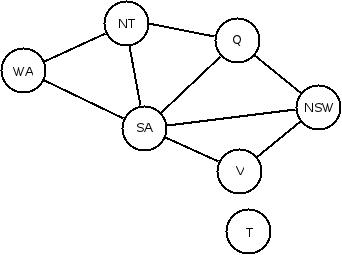
\includegraphics[scale=.5]{img/Australia.jpeg}
\caption{Esempio di grafo, colorazione della mappa australiana.}
\end{figure}

Si può dare una \emph{formulazione incrementale} di un CSP come se fosse un
problema di ricerca:
\begin{itemize}
\item[-]\textbf{Stato iniziale}: l'assegnamento vuoto $\{\}$ nel quale
nessuna variabile ha un valore assegnato.
\item[-]\textbf{Funzione successore}: assegna un valore ad una variabile
in modo  che
non violi alcun vincolo ad essa associato.
\item[-]\textbf{Test obiettivo}: verifica che l'assegnamento sia completo.
\item[-]\textbf{Costo di cammino}: costante per ogni passo.
\end{itemize}

Poiché una soluzione deve essere un assegnamento completo avrà almeno profondità
$n$, dove $n$ è il numero di variabili coinvolte. Per questo, per risolvere i
CSP sono molto utilizzati gli algoritmi di ricerca in profondità.

\`E quindi possibile definire una \emph{formulazione a stato completo} del
problema, nella quale ogni stato è un assegnamento completo che può soddisfare
i vincoli oppure no. Questo approccio è utilizzato negli algoritmi di ricerca
locale, nei quali viene assegnato un valore ad ogni variabile per lo stato
iniziale e normalmente la funzione successore cambia il valore di una variabile
alla volta.

\section{Un semplice esempio: colorazione di una mappa}
Si è definito formalmente un problema di soddisfacimento di vincoli e si è
quindi spiegato brevemente cosa significa risolverlo. A questo punto vediamo un
classico esempio: la colorazione di mappe geografiche.

La colorazione delle regioni di uno stato su una mappa geografica può essere
facilmente espresso mediante un CSP, prendiamo come esempio la mappa
dell'Australia (esempio trattato in \cite{intArt}).

\subsection{Definizione del problema}
Innanzitutto occorre stabilire qual'è il problema. Colorare le regioni di un
paese in modo che non si confondano significa che quelle adiacenti devono
avere colori differenti. Supponiamo di avere a disposizione solo tre colori:
rosso, verde e blu. Le regioni dell'Australia sono sette: Western Australia,
Northern Territory, South Australia, Queensland, New South Wales, Victoria
e l'isola della Tasmania. In figura \ref{figAustralia} si notano le varie
regioni sotto forma di nodi del grafo dei vincoli, gli archi rappresentano la
relazione di
confine tra regioni.

A questo punto abbiamo tutti gli elementi per ottenere un problema
$\mathbf{P} = \left\langle \mathbf{V}, \mathbf{D}, \mathbf{C}\right\rangle$
tale che:
\[
\mathbf{V} = \left\{ W_A, N_T, S_A, Q, N_{SW}, V, T \right\},
\]
\[
\mathbf{D} =  \left\{\textrm{rosso},\textrm{verde},\textrm{blu}\right\},
\]
in cui i vincoli appartenenti a $\mathbf{C}$, descritti dagli archi del grafo,
sono del tipo:
\[
\mathcal{C}_1 \leftarrow  W_A \neq N_T, \quad \mathcal{C}_2 \leftarrow  W_A
\neq S_A,\quad \ldots
\]

\subsection{Dalla definizione formale alla realizzazione in Java mediante
JSR-331}
Come già accennato nella sezione precedente la definizione formale di un
CSP e la sua soluzione sono concetti abbastanza generici da poter essere
applicati a qualunque sistema di risolutori o linguaggio di programmazione.

Tuttavia la sintassi può essere molto differente tra un linguaggio e l'altro, ma
anche tra un risolutore e un altro scritti nel medesimo linguaggio, la
specifica JSR-331 si prefigge di standardizzare tale sintassi mediante
la definizione di un'interfaccia. Vediamo come può essere rappresentato
il problema dell'Australia.

\begin{lstlisting}[language=Java,
                   caption = {\files{Australia.java}.}]
public class Australia {
  static final String[] colors = { "red", "green", "blue"};
...
}
\end{lstlisting}
Viene creata la classe \files{Australia} in cui verrà definito il problema
e la chiamata al risolutore di vincoli. L'array di stringhe rappresenta
il dominio delle variabili che verranno create.

\begin{lstlisting}[language=Java,
                   caption = {definizione delle variabili.},
                   frame = shadowbox]
static public void main(String[] argv) {
  try {
    Problem p = new Problem("Australia");
    // Variabili.
    int n = colors.length-1;
    Var WA   = p.variable("Western Australia",0, n);
    Var NT   = p.variable("Northern Territory", 0, n);
    Var SA   = p.variable("South Australia",0, n);
    Var Q    = p.variable("Queensland",0, n);
    Var NSW  = p.variable("New South Wales",0, n);
    Var V    = p.variable("Victoria",0, n);
    Var T    = p.variable("Tasmania",0, n);
\end{lstlisting}
In questa parte di codice viene creato il problema \files{p} chiamato
``Australia''
e vengono quindi create le variabili legate al problema (costruite dal
metodo \files{variable(nome, min, max)} della classe \files{Problem}).

Si noti che il dominio delle variabili è specificato nella chiamata del metodo
\files{variable}, ovvero ogni variabile ha dominio $[0, n-1]$, in cui $n$ è
la lunghezza del vettore dei domini. Le variabili si riferiscono in pratica agli
indici di tale vettore.

\begin{lstlisting}[language=Java,
                   caption = {definizione dei vincoli.},
                   frame = shadowbox]
    // Vincoli.
    p.post(WA, "!=", NT);
    p.post(WA, "!=", SA);
    p.post(NT, "!=", SA);
    p.post(NT, "!=", Q);
    p.post(SA, "!=", Q);
    p.post(SA, "!=", NSW);
    p.post(SA, "!=", V);
    p.post(Q, "!=", NSW);
    p.post(V, "!=", NSW);
\end{lstlisting}
La definizione dei vincoli avviene mediante il metodo
\files{post(Var, String, Var)}, sempre invocato sul problema. In questo caso
vengono specificati tutti i vincoli di disuguaglianza come specificato in figura
\ref{figAustralia}.

\begin{lstlisting}[language=Java,
                   caption = {ricerca della soluzione.},
                   frame = shadowbox]
Solution solution = p.getSolver().findSolution();
if (solution != null) {
  for (int i = 0; i < p.getVars().length; i++) {
    Var var = p.getVars()[i];
    p.log(var.getName() + " - " +
    colors[solution.getValue(var.getName())]);
  }
}
else
  p.log("no solution found");
\end{lstlisting}
Dopo aver trovato la soluzione, viene stampata mediante
un semplice algoritmo (che ovviamente non fa parte dello standard) e questo è
il risultato ottenuto con JSetL:
\begin{lstlisting}[caption = {la soluzione.},
                   frame = shadowbox]
Western Australia - red
Northern Territory - green
South Australia - blue
Queensland - red
New South Wales - green
Victoria - red
Tasmania - red
\end{lstlisting}

\hyphenation{
sil-la-ba-zio-ne
JSetL
Choco
JaCoP
}

\chapter{Java Specification Request 331}\label{capJSR}
JSR-331 è una \emph{richiesta per specifiche} Java in fase di sviluppo sotto
le regole redatte dal Java Community Process. Queste specifiche definiscono
le API per la programmazione a vincoli.

La specifica JSR-331 risponde alla necessità di ridurre i costi associati 
all'incorporazione di risolutori di vincoli (come JSetL, Choco, etc.) ad
applicazioni commerciali e non, operanti nel mondo reale. Esiste già un 
certo numero di fornitori di queste API, come già accennato possiamo
ricordare JSetL, Choco, JaCoP ed altri. Tuttavia le differenze tra questi
sono abbastanza significative da causare gravi difficoltà di utilizzo per 
gli sviluppatori di software.

\section{Obiettivi del JSR-331}
La standardizzazione della programmazione a vincoli si prefigge come scopo
quello di rendere tale tecnologia più accessibile per gli sviluppatori.
Avendo un'interfaccia unificata sarà possibile, per i programmatori, modellare
il problema in modo tale da poter provare la soluzione con più CP solver.
Questo minimizza la dipendenza da fornitori specifici, ma allo stesso
tempo non limita la possibilità di quest'ultimi nel procedere con lo sviluppo
del solver.

Gli obiettivi delle specifiche sono:
\begin{itemize}
\item[-]facilitare l'inserimento della tecnologia basata sui vincoli nelle 
applicazioni Java;
\item[-]aumentare la comunicazione e la standardizzazione tra i vari fornitori
di CP solver;
\item[-]incoraggiare il mercato delle applicazioni basate sulla programmazione
a vincoli e dei suoi strumenti mediante la standardizzazione delle suddette API;
\item[-]facilitare l'integrazione di tecniche basate sui vincoli in altri
JSR per supportare la programmazione dichiarativa;
\item[-]rendere le applicazioni Java più portabili tra vari fornitori di
risolutori di vincoli;
\item[-]fornire un modello per l'implementazione ed il supporto di
librerie di vincoli e strategie di ricerca per diverse applicazioni basate sulla
programmazione a vincoli;
\item[-] supportare i fornitori di solver offrendo API che vadano incontro alle
loro necessità e che siano di facile implementazione.
\end{itemize}

\subsection{A chi è rivolta?}
La specifica è rivolta principalmente a tre soggetti:
\begin{itemize}
\item[-]aziende che utilizzano le CP API
per sviluppare applicazioni di supporto a decisioni in ambito industriale;
\item[-]fornitori di risolutori di vincoli che intendono sviluppare e mantenere
la propria implementazione delle CP API;
\item[-]ricercatori in ambito di programmazione a vincoli che vogliono 
fornire o arricchire librerie di vincoli standard, algoritmi di ricerca e
problemi concreti che vengano mantenuti dalla CP community.
\end{itemize}

\subsection{Scopo della specifica}
Lo scopo della specifica JSR-331 è di definire un'interfaccia semplice da
utilizzare, leggera e che costituisca uno standard per acquisire ed utilizzare
risolutori di vincoli.

La specifica è mirata a piattaforme basate su Java ed è compatibile con JDK 1.5
o successivi.

L'ambito della specifica segue un approccio minimalista, con particolare cura
alla facilità d'uso. Ricopre i più comuni concetti dei problemi con vincoli e
della loro rappresentazione che è ormai già diventata una standardizzazione
di fatto, adottata dai solver e negli articoli scientifici. Tale ambito è
allo stesso tempo sufficientemente ampio da permettere agli sviluppatori di
applicazioni l'utilizzo delle interfacce standard per modellare
e risolvere tipici problemi di soddisfacimento di vincoli, all'interno
dei domini più comuni in ambito aziendale, come la pianificazione, l'allocazione
delle risorse e la configurazione.

I seguenti concetti ed oggetti rappresentano l'ambito iniziale delle
specifiche:
\begin{itemize}
\item[-]variabili vincolate dei tipi più utilizzati: interi, booleani, reali
ed insiemi di interi;
\item[-]vincoli unari e binari ed espressioni definite con variabili vincolate;
\item[-]i più comuni vincoli globali;
\item[-]la possibilità di ottenere una soluzione, ogni soluzione oppure
una soluzione ottimale, sotto certi limiti definiti dall'utente.
\end{itemize}

Ci si aspetta che le API vengano ampliate e così è anche specificato come
aggiungere nuovi concetti, funzionalità e strategie relative ai CP nel momento
in cui queste vengono comunemente adottate.

JSR-331 è focalizzato solo sull'interfaccia, per quanto riguarda le 
implementazioni non assume nessun approccio particolare. I seguenti concetti ed
oggetti sono prerogativa esclusiva dei vari solver e strumenti specifici:
\begin{itemize}
\item[-]meccanismi d'implementazione per i vari domini;
\item[-]implementazione dei più comuni vincoli binari e globali;
\item[-]meccanismi di propagazione di vincoli;
\item[-]backtracking e meccanismi di reversibilità.
\end{itemize}

\section{Struttura}
JSR-331 prescrive un insieme di operazioni fondamentali per definire e risolvere
problemi di soddisfacimento di vincoli e problemi di ottimizzazione.
La struttura consiste in tre principali componenti:
\begin{itemize}
\item[-]specifiche (CP API);
\item[-]implementazione basata su differenti CP solver;
\item[-]\emph{TCK} (\emph{Tecnology Compatibility Kit}), un pacchetto di test,
strumenti e
documentazione che verrà utilizzato per verificare la conformità alle
specifiche delle varie implementazioni.
\end{itemize}

Ogni implementazione del JSR-331 può implementare l'interfaccia direttamente
oppure può estendere le classi della \emph{common implementation} fornite
dalle API. La common implementation può essenzialmente semplificare
l'implementazione del JSR-331. Nel momento in cui lo standard diverrà più 
maturo e più
implementazioni adotteranno vincoli e strategie di ricerca comuni, queste
verranno gradualmente aggiunte alle librerie della common implementation.

\subsection{Specifiche}
Le specifiche per JSR-331 consistono in:
\begin{itemize}
\item[-]un'interfaccia pura (\files{javax.constraints});
\item[-]la common implementation (\files{javax.constraints.impl}).
\end{itemize}

\begin{itemize}
\item[-]\files{javax.constraints} 

Interfacce Java pure, come \files{Problem} o
\files{Solver}, che specificano i maggiori concetti e metodi per definire e 
risolvere problemi di soddisfacimento ed ottimizzazione di vincoli.

\item[-]\files{javax.constraints.impl}

Classi Java come \files{AbstractProblem} e 
\files{AbstractSolver} che implementano (parzialmente o completamente)
definizioni di problemi, concetti di risoluzione e metodi che non
dipendono direttamente da uno specifico CP solver.
\end{itemize}

\subsection{Implementazioni per JSR-331}
Ogni implementazione della specifica JSR-331 è basata su un 
CP solver (come ad esempio JSetL) e deve fornire le definizioni per tutte le
interfacce presenti nel pacchetto \files{javax.constraints}.
Alcune classi possono essere implementate direttamente dall'interfaccia
standard, altre si possono ottenere estendendo l'implementazione comune
fornita dal pacchetto \files{javax.constraints.impl}. 

JSR-331 richiede
che ogni implementazione fornisca almeno la definizione delle classi
presenti nei seguenti pacchetti:
\begin{itemize}
\item[-]\files{javax.constraints.impl}

Classi Java come \files{Problem} o \files{Solver} 
che forniscono
una implementazione finale per la definizione di problemi, concetti
e metodi. Queste classi possono essere derivate dall'implementazione
comune.

\item[-]\files{javax.constraints.impl.constraint}

Una libreria di vincoli che contiene
le implementazioni di vincoli basilari e globali che sono di fatto basati
sulle varie implementazioni dei CP solver.

\item[-]\files{javax.constraints.impl.search}

Una libreria di strategie di ricerca che contiene 
le implementazioni basate sui solver concreti.
\end{itemize}

In aggiunta ogni implementazione può fornire propri vincoli (nativi) e
proprie strategie di ricerca, assumendo che questi seguano le interfacce 
standard \files{javax.constraints.Constraint} e 
\files{javax.constraints.SearchStrategy}.

Il fatto che ogni implementazione per JSR-331 debba adottare gli stessi
nomi per i package, per le principali classi e metodi permetterà agli 
sviluppatori di applicazioni di passare facilmente da un solver ad
un altro (differenti implementazioni) senza  dover cambiare nulla nel proprio
codice. Possono di fatto scrivere applicazioni specifiche, motori basati su
vincoli una sola volta utilizzando le CP API e quindi utilizzare i differenti 
solver cambiando solo i file \files{.jar} all'interno del classpath.

\begin{nota}
La possibilità di cambiare i solver senza modificare il codice delle 
applicazioni ha comunque una limitazione: fissando  per convenzione i nomi
dei package si ha come effetto collaterale quello di non poter unire
le funzionalità di due o più solver differenti. La scelta di una determinata 
implementazione sottostante è definita dal solo file \files{.jar} nel
classpath dell'applicazione.
\end{nota}

\subsection{Tecnology Compatibility Kit}
Il \emph{TCK} (\emph{Tecnology Compatibility Kit}) è un pacchetto di 
documentazione, test e  strumenti utilizzati per testare la correttezza delle 
implementazioni per le specifiche di JSR-331.

Il TCK consiste in due package:
\begin{itemize}
\item[-]\files{org.jcp.jsr331.tests}

Contiene i moduli 
JUnit che permettono all'utente di validare automaticamente la correttezza
dell'implementazione con la specifica JSR-331.

\item[-]\files{org.jcp.jsr331.samples}

Contiene esempi di CSP che 
forniscono test integrati per i più comuni vincoli e
strategie di ricerca incluse in JSR-331, mostrano l'utilizzo della
programmazione a vincoli per problemi reali.
\end{itemize}

Non tutti i concetti introdotti nel package \files{javax.constraints} sono
richiesti per l'implementazione del solver al fine di essere validato.
Il pacchetto \files{org.jcp.jsr331.tests} contiene solo quei test che
sono normativi per la specifica (devono essere soddisfatti da ogni
implementazione al fine di essere validate). Il file 
\files{AllTests.java} all'interno del package contiene tutti i test normativi.

Il pacchetto \files{javax.constraints.impl} fornisce le implementazioni di
base per alcune interfacce e metodi opzionali. Ci sono due tipi di
implementazioni opzionali:
\begin{enumerate}
\item implementazioni di default (non le più efficienti) che possono
essere sovrascritte da una particolare implementazione per JSR-331;
\item semplici frammenti di codice che lanciano un'eccezione a runtime e che 
informano l'utente che quel metodo non è stato implementato dalla
particolare implementazione.
\end{enumerate}

\begin{nota}
Il package \files{org.jcp.jsr331.samples} è presente a soli fini dimostrativi e
non tutto ciò che è ivi incluso deve essere supportato da ogni implementazione.
\end{nota}

\subsection{Modello di sviluppo}
Il modello di sviluppo per le applicazioni finali che utilizzeranno le
API JSR-331 richiederà che i seguenti file \files{.jar} siano inclusi nel 
classpath:
\begin{itemize}
\item[-]\files{jsr331.jar}: include tutte le classi e le interfacce standard;
\item[-]\files{jsr331.<solver>.jar}: include tutte le classi della specifica
implementazione;
\item[-]\files{<solver>.jar}: include tutte le classi del solver utilizzato su 
cui si basa l'implementazione.
\end{itemize}
Ad esempio lo sviluppo basato su JSetL richiederà:
\begin{itemize}
\item[-]\files{jsr331.jar}
\item[-]\files{jsr331.jsetl.jar}
\item[-]\files{jsetl.jar}
\end{itemize}

\section{Rappresentazione di un CSP}
Come si è evidenziato nel capitolo \ref{capCP} un CSP è definito da un insieme
di variabili con il relativo dominio ed un insieme di vincoli; a queste 
variabili viene quindi ristretto il dominio per trovare una o più soluzioni.

JSR-331 definisce tutti i concetti Java per la \emph{rappresentazione} e la
\emph{risoluzione} di un problema di soddisfacimento di vincoli. Suddivide
quindi in maniera naturale un CSP in due parti fondamentali:
\begin{itemize}
\item[-]la \textbf{definizione} del problema, rappresentata dall'interfaccia
\files{Problem};
\item[-]la \textbf{soluzione} del problema, rappresentata dall'interfaccia
\files{Solver}. 
\end{itemize}  

Ogni concetto fondamentale di un CSP appartiene ad una delle due categorie, a
livello utente è possibile presentare un CSP mediante la seguente suddivisione:
\begin{enumerate}\samepage
\item Problema:
  \begin{itemize}
  \item[(a)]Variabili vincolate.
  \item[(b)]Vincoli.
  \end{itemize}
\item Risoluzione:
  \begin{itemize}
  \item[(c)]Strategia.
  \item[(d)]Soluzione.
  \end{itemize}
\end{enumerate}

Ogni CP solver utilizza nomi e rappresentazioni differenti per questi concetti,
che comunque sono semanticamente invarianti per la maggior parte di essi.
JSR-331 fornisce una nomenclatura unificata e specifiche dettagliate.

La definizione di un problema non conosce nulla a riguardo della sua 
risoluzione. Un'istanza della classe \files{Problem} può quindi esistere a
prescindere dall'esistenza di un'istanza di \files{Solver}. Non vale il
viceversa, poiché un'istanza della classe \files{Solver} può essere creata
solo partendo da uno specifico problema. Durante la ricerca di una soluzione
il solver può cambiare lo stato del problema (modifica dei domini delle 
variabili, semplificazione dei vincoli, etc). \`E quindi responsabilità
degli specifici risolutori mantenere (o meno) i possibili stati del problema in
base alla strategia di ricerca utilizzata.

\hyphenation{
un'es-pres-sio-ne
JSetL
Choco
JaCoP
}
\chapter{La Libreria JSetL}\label{jsetl}
In questo capitolo verrà descritta brevemente la libreria JSetL, soffermandosi
principalmente sull'utilizzo, ovvero sui costrutti e i metodi utilizzati
nell'implementazione concreta di JSR-331. 

JSetL è una libreria Java che combina il paradigma di programmazione orientato 
agli oggetti con i concetti dei linguaggi \emph{CLP} (\emph{Constraint Logic 
Programming}), 
come variabili logiche, elenchi,
unificazione, risoluzione di vincoli, non determinismo.

Tra le caratteristiche di interesse per l'implementazione JSR-331 troviamo le
variabili logiche (\files{IntLVar} e \files{SetLVar}), i vincoli 
(\files{Constraint}) ed il meccanismo di risoluzione dei vincoli 
(\files{SolverClass}).

\section{Variabili logiche}
JSetL supporta la nozione di variabile logica come quella che si trova in
Logica e nei linguaggi di programmazione funzionale. Le variabili logiche 
possono essere sia \emph{inizializzate} che \emph{non inizializzate}.
Il valore di una variabile logica in JSetL può essere di qualsiasi tipo.
Un valore può essere assegnato ad una variabile logica (non inizializzata) come
risultato dell'elaborazione dei vincoli che la coinvolgono.

\begin{flushleft}\textbf{Variabile logica.}\\
Una \emph{variabile logica} è un'istanza della classe \files{LVar}, creata
dalla seguente chiamata:
\begin{center}
\lstinline[language = Java]$LVar varName = new LVar(ExtVarName, VarValue);$
\end{center}
dove \files{varName} è il nome della variabile, \files{ExtVarName} è il nome
opzionale esterno e \files{VarValue} è un parametro opzionale che ne
rappresenta il valore.
\end{flushleft}

Il nome esterno è una stringa che può essere utile quando occorre stampare la
variabile ed i possibili vincoli che la coinvolgono. 

\begin{nota}
Durante la fase di sviluppo dell'implementazione la stampa è stata una parte 
fondamentale per il debugging, sia per quanto riguarda le prove d'esecuzione che
per i test con JUnit e con il TCK. Ovviamente il nome esterno non definisce
una variabile (essendo opzionale) e sarebbe possibile creare variabili con
il medesimo \files{ExtVarName} ma indipendenti. Tuttavia, per 
facilitare il riconoscimento all'occhio umano è buona norma definire nomi
significativi, per quanto riguarda i nomi delle variabili temporanee interne
si rimanda alla sezione \ref{problem}.
\end{nota}

\section{Variabili logiche intere}
Le variabili logiche intere sono quelle d'interesse al fine di implementare le 
classi  \files{Var} e \files{VarBool} per l'attuale implementazione JSR-331. 

In JSetL le variabili intere sono rappresentate
dalla classe \files{IntLVar}, che di fatto estende la
classe \files{LVar} ereditandone metodi e costruttori.

\begin{flushleft}\textbf{Variabile logica intera.}\\
Una \emph{variabile logica intera} è un'istanza della classe \files{IntLVar}, 
creata dalla seguente chiamata:
\begin{center}
\lstinline[language = Java]$IntLVar varName = new IntLVar(name);$
\end{center}
dove  \files{varName} è il nome della variabile e \files{name} è il nome
esterno opzionale.
\end{flushleft}

\subsection{Dominio}
Ogni variabile logica intera ha un dominio ad essa associato, nel caso di
\files{IntLVar} il dominio è rappresentato da un multi-intervallo di interi.

Il concetto di multi-intervallo è definito in \cite{tesiAmadini} e, in breve, è
costituito dall'unione disgiunta di intervalli di interi. Ogni volta che
la variabile in questione viene modificata tramite vincoli che la coinvolgono
il relativo dominio viene modificato di conseguenza.

\subsection{Metodi utili}
La classe \files{IntLVar} fornisce alcuni metodi di utilità, quelli più
utilizzati nell'implementazione sono:
\begin{itemize}
\item[-]\files{MultiInterval getDomain()}: restituisce il
dominio della variabile intera.
\item[-]\files{Boolean isBound()}: restituisce 
\verb true  se
il dominio è ristretto ad un solo elemento, \verb false  in caso contrario.
\end{itemize}

\subsection{Operazioni aritmetiche}
\`E possibile creare variabili vincolate intere anche partendo da una
variabile d'invocazione (\files{this}), mediante le comuni operazioni
aritmetiche. Siano $X_0$ la variabile d'invocazione \files{x0}, $\mathcal{C}_0$ 
i vincoli ad essa associati, $X_1$ la variabile data dal parametro \files{x1}, 
$\mathcal{C}_1$ i vincoli ad essa associati, $X_2$ la nuova variabile \files{x2}
ottenuta dalle seguenti operazioni:
\begin{itemize}
\item[-]\files{IntLVar sum(Integer k)}: crea una variabile logica intera 
vincolata \files{x2} tale che se \files{x2 = x0.sum(k)}, allora:
\[
X_2 = X_0 + k \wedge \mathcal{C}_0.
\]
\item[-]\files{IntLVar sum(IntLVar x1)}: crea una variabile logica intera 
vincolata tale che se \files{x2 = x0.sum(x1)}, allora:
\[
X_2 = X_0 + X_1 \wedge \mathcal{C}_0 \wedge \mathcal{C}_1.
\]
\item[-]\files{IntLVar sub(Integer k)}: crea una variabile logica intera 
vincolata tale che se \files{x2 = x0.sub(k)}, allora:
\[
X_2 = X_0 - k \wedge \mathcal{C}_0.
\]
\item[-]\files{IntLVar sub(IntLVar x1)}: crea una variabile logica intera 
vincolata tale che se \files{x2 = x0.sub(x1)}, allora:
\[
X_2 = X_0 - X_1 \wedge \mathcal{C}_0 \wedge \mathcal{C}_1.
\]
\item[-]\files{IntLVar mul(Integer k)}: crea una variabile logica intera 
vincolata tale che se \files{x2 = x0.mul(k)}, allora:
\[
X_2 = X_0 \cdot k \wedge \mathcal{C}_0.
\]
\item[-]\files{IntLVar mul(IntLVar x1)}:  crea una variabile logica intera 
vincolata tale che se \files{x2 = x0.mul(x1)}, allora:
\[
X_2 = X_0 \cdot X_1 \wedge \mathcal{C}_0 \wedge \mathcal{C}_1.
\] 
\item[-]\files{IntLVar div(Integer k)}: crea una variabile logica intera 
vincolata tale che se \files{x2 = x0.div(k)}, allora:
\[
X_2 = \frac{X_0}{k} \wedge k \neq 0 \wedge \mathcal{C}_0.
\]
\item[-]\files{IntLVar div(IntLVar x1)}:  crea una variabile logica intera 
vincolata tale che se \files{x2 = x0.div(x1)}, allora:
\[
X_2 = \frac{X_0}{X_1} \wedge X_1 \neq 0 \wedge \mathcal{C}_0 \wedge 
\mathcal{C}_1.
\]
\end{itemize}

\subsection{Vincoli}
La classe \files{IntLVar} fornisce metodi per la creazione dei comuni vincoli
che rappresentano le relazione su interi ($<$, $=$, $\neq$, \ldots). 
Inoltre fornisce altri
vincoli comunemente usati come \emph{AllDifferent}, vincoli di dominio e di
appartenenza.

Di seguito si elencano e descrivono brevemente i vincoli utilizzati 
nell'implementazione, siano
$X_0$ la variabile d'invocazione \files{this}, $\mathcal{C}_0$ i vincoli ad 
essa associati, $X_1$ la variabile data dal parametro \files{x1} e 
$\mathcal{C}_1$ i relativi vincoli associati:
\begin{itemize}
\item[-]\files{Constraint eq(Integer k)}: 
crea un nuovo vincolo $\mathcal{C}$ tale che:
\[
\mathcal{C} \leftarrow X_0 = k \wedge \mathcal{C}_0.
\]
\item[-]\files{Constraint eq(IntLVar x1)}: crea un nuovo vincolo $\mathcal{C}$ 
tale che:
\[
\mathcal{C} \leftarrow X_0 = X_1 \wedge \mathcal{C}_0 \wedge \mathcal{C}_1.
\]
\item[-]\files{Constraint neq(Integer k)}: 
crea un nuovo vincolo $\mathcal{C}$ tale che:
\[
\mathcal{C} \leftarrow X_0 \neq k \wedge \mathcal{C}_0.
\]
\item[-]\files{Constraint neq(IntLVar x1)}: crea un nuovo vincolo $\mathcal{C}$ 
tale che:
\[
\mathcal{C} \leftarrow X_0 \neq X_1 \wedge \mathcal{C}_0 \wedge \mathcal{C}_1.
\]
\item[-]\files{Constraint le(Integer k)}: 
crea un nuovo vincolo $\mathcal{C}$ tale che:
\[
\mathcal{C} \leftarrow X_0 \leq k \wedge \mathcal{C}_0.
\]
\item[-]\files{Constraint le(IntLVar x1)}: crea un nuovo vincolo $\mathcal{C}$ 
tale che:
\[
\mathcal{C} \leftarrow X_0 \leq X_1 \wedge \mathcal{C}_0 \wedge \mathcal{C}_1.
\]
\item[-]\files{Constraint lt(Integer k)}: 
crea un nuovo vincolo $\mathcal{C}$ tale che:
\[
\mathcal{C} \leftarrow X_0 < k \wedge \mathcal{C}_0.
\]
\item[-]\files{Constraint lt(IntLVar x1)}: crea un nuovo vincolo $\mathcal{C}$ 
tale che:
\[
\mathcal{C} \leftarrow X_0 < X_1 \wedge \mathcal{C}_0 \wedge \mathcal{C}_1.
\]
\item[-]\files{Constraint ge(Integer k)}: 
crea un nuovo vincolo $\mathcal{C}$ tale che:
\[
\mathcal{C} \leftarrow X_0 \geq k \wedge \mathcal{C}_0.
\]
\item[-]\files{Constraint ge(IntLVar x1)}: crea un nuovo vincolo $\mathcal{C}$ 
tale che:
\[
\mathcal{C} \leftarrow X_0 \geq X_1 \wedge \mathcal{C}_0 \wedge \mathcal{C}_1.
\]
\item[-]\files{Constraint gt(Integer k)}: 
crea un nuovo vincolo $\mathcal{C}$ tale che:
\[
\mathcal{C} \leftarrow X_0 > k \wedge \mathcal{C}_0.
\]
\item[-]\files{Constraint gt(IntLVar x1)}: crea un nuovo vincolo $\mathcal{C}$ 
tale che:
\[
\mathcal{C} \leftarrow X_0 > X_1 \wedge \mathcal{C}_0 \wedge \mathcal{C}_1.
\]
\end{itemize}

Sia \files{vars} un vettore di $n+1$ variabili logiche intere tale che $X_0$
rappresenti \files{vars[0]}, $X_1$ rappresenti \files{vars[1]}, etc.
Il vincolo ``AllDifferent'' è descrivibile come:
\begin{itemize}
\item[-]\files{Constraint AllDifferent(IntLVar[] vars)}: crea un nuovo vincolo 
$\mathcal{C}$ tale che:
\[
\mathcal{C} \leftarrow X_0 \neq X_1 \wedge X_0 \neq X_2 \wedge \cdots \wedge X_0
\neq X_n \wedge X_1 \neq X_2 \wedge \cdots \wedge X_1 \neq X_n \wedge \cdots
\]
è possibile scrivere in modo più compatto il vincolo:
\[
\mathcal{C} \leftarrow \left(\bigwedge_{0 \leq i < j \leq n} X_i \neq X_j\right)
\wedge \bigwedge_{i = 0}^{n}\mathcal{C}_i.
\]
\end{itemize}

\section{Variabili logiche su insiemi di interi}
Le variabili logiche di interesse al fine di implementare la classe 
\files{VarSet} per l'attuale implementazione JSR-331 sono
quelle di insiemi di interi. 

In JSetL le variabili di insiemi di interi sono rappresentate dalla classe
\files{SetLVar}, che estende la classe \files{LVar} ereditandone metodi e 
costruttori.

\begin{flushleft}\textbf{Variabile logica su insiemi di interi.}
Una variabile logica su \emph{insiemi di interi} (più brevemente un 
\emph{insieme di interi}) è un'istanza di
\files{SetLVar}, 
creata dalla seguente chiamata:
\begin{center}
\lstinline[language = Java]!SetLVar varName = new SetLVar(name);!
\end{center}
dove  \files{varName} è il nome della variabile e \files{name} è il nome
opzionale esterno.
\end{flushleft}

\subsection{Dominio}
Il dominio di un \files{SetLVar} è rappresentato da un'istanza di
\files{SetInterval} che di fatto è un reticolo\footnote{Un reticolo è un 
insieme parzialmente ordinato in cui ogni coppia di elementi ha sia un estremo 
inferiore che un estremo superiore.} di insiemi di interi 
(\files{Set<Integer>}).

Il dominio di una variabile di insiemi di interi può essere specificato alla
creazione della variabile, ed è modificato automaticamente quando vengono
risolti i vincoli ad essa associati.

Quando il dominio di una variabile si restringe fino ad essere rappresentato da
un singoletto, la variabile viene detta \emph{bound}, se
invece il dominio si restringe all'insieme vuoto significa che i vincoli ad
essa associati sono insoddisfacibili.

Sia \files{s} un'istanza della classe \files{MultiInterval} che rappresenta un
insieme di interi $S$, la variabile logica che ha come dominio $S$ è creata 
dalla seguente chiamata:
\begin{center}
\lstinline[language = Java]!SetLVar varName = new SetLVar(s);!
\end{center}

\subsection{Metodi utili}
La classe \files{SetLVar} fornisce alcuni metodi utili ereditati dalla classe
\files{LVar}, adattati per supportare i tipi di ritorno 
\files{MultiInterval}, \files{SetLVar} e per i vincoli su insiemi e domini.
\begin{itemize}
\item[-]\files{Constraints getConstraints()}: restituisce la congiunzione di
tutti i vincoli associati alla variabile;
\item[-]\files{MultiInterval getDomain()}: restituisce il
dominio della variabile;
\item[-]\files{Boolean isBound()}: restituisce 
\files{true}  se
il dominio è ristretto ad un solo elemento, \files{false}  in caso contrario.
\end{itemize}

\subsection{Operazioni insiemistiche}
Come nel caso delle variabili intere, è possibile creare nuove
variabili insiemistiche utilizzando metodi che riproducono le comuni operazioni
sugli insiemi. Sia $S_0$ l'insieme rappresentante la variabile d'invocazione
\files{s},
$\mathcal{C}_0$ i vincoli ad essa associati, siano $S_1$, $S_2$ gli insiemi
rappresentanti i parametri \files{SetLVar x} e \files{y}, $\mathcal{C}_1$ e
$\mathcal{C}_2$  i vincoli ad esse associati, si definiscono le seguenti 
operazioni:
\begin{itemize}
\item[-]\files{SetLVar compl()}: 
crea un nuovo insieme di interi tale che, se \files{x = s.compl()}
allora:
\[
S_1 = S_0^c \wedge \neg  \mathcal{C}_0;
\]
\item[-]\files{SetLVar intersect(SetLVar y)}: crea un nuovo insieme di interi
tale che, se \files{x = s.intersect(y)} allora:
\[
S_1 = S_0 \cap S_2 \wedge \mathcal{C}_0 \wedge \mathcal{C}_2;
\]
\item[-]\files{SetLVar union(SetLVar y)}: crea un nuovo insieme di interi
tale che, se \files{x = s.union(y)} allora:
\[
S_1 = S_0 \cup S_2 \wedge \mathcal{C}_0 \vee \mathcal{C}_2;
\]
\item[-]\files{SetLVar diff(SetLVar y)}: crea un nuovo insieme di interi
tale che, se \files{x = s.diff(y)} allora:
\[
S_1 = S_0 \setminus S_2 \wedge \mathcal{C}_0 \wedge \neg \mathcal{C}_2.
\]
\end{itemize}


%% Vincoli
\section{Vincoli}
JSetL fornisce vincoli per specificare condizioni su variabili logiche e 
insiemi. Questi vincoli sono manipolati da un \emph{risolutore di vincoli} 
(un'istanza della classe \files{SolverClass}) che implementa le specifiche
strategie di risoluzione.

Il \emph{dominio dei vincoli} in JSetL è il dominio $\mathcal{SET}$ definito
in \cite{artClp}, esteso con alcuni nuovi vincoli per la comparazione tra 
interi.
\begin{flushleft}\textbf{Vincolo atomico}.\\
Un \emph{vincolo atomico} in JSetL è un'espressione in una delle 
seguenti forme:
\begin{itemize}
\item[-] $e_1.\texttt{op}(e_2)$;
\item[-] $e_1.\texttt{op}(e_2, e_3)$;
\end{itemize}
dove \files{op}  è uno dei metodi predefiniti (\files{eq, neq, in, nin},
\ldots) ed $e_1$, $e_2$, $e_3$ sono espressioni il cui tipo dipende da 
\files{op}.
\end{flushleft}

Il significato di questi metodi è associato in modo naturale al loro stesso 
nome, ovvero \files{eq} e \files{neq} stanno ad indicare l'uguaglianza e la
disuguaglianza rispettivamente (dall'inglese equal e not equal),
\files{in} e \files{nin} per l'appartenenza e la non appartenenza, etc.

\begin{flushleft}\textbf{Vincolo}.\\
Un \emph{vincolo} è un vincolo atomico o (ricorsivamente) un'espressione
del tipo:
\[
c_1.\files{and}(c_2.\files{and}(\cdots c_{n-1}.\files{and}(c_n) \cdots)
\]
\[
\textrm{oppure}
\]
\[
c_1.\files{and}(c_2). \ldots .\files{and}(c_n)
\]
dove $c_1, c_2, \ldots, c_n$ sono vincoli atomici.
\end{flushleft} 
Il significato di $c_1.\files{and}(c_2). \ldots .\files{and}(c_n)$ è la 
congiunzione logica $\mathcal{C}_1 \wedge \mathcal{C}_2 \wedge \cdots 
\wedge \mathcal{C}_n$, in cui i $\mathcal{C}_i$ sono le espressioni logiche
rappresentanti i vincoli atomici $c_i$.

\begin{flushleft}\textbf{Constraint.}\\
Un \emph{Constraint} JSetL è un'istanza della classe \files{Constraint}, creata
dalla seguente chiamata:
\begin{center}
\lstinline[language = Java]
$Constraint constraintName = new Constraint();$
\end{center}
dove \files{constraintName} è il nome del vincolo.
\end{flushleft}

\subsection{Operazioni logiche}
\`E possibile creare vincoli anche partendo da un
vincolo d'invocazione (\files{this}), mediante le comuni operazioni
logiche. Siano  $\mathcal{C}_1$, 
$\mathcal{C}_2$ i vincoli rappresentanti le istanze dei \files{Constraint c1}
e \files{c2}. Si definiscono le seguenti operazioni logiche:
\begin{itemize}
\item[-]\files{Constraint c = c1.and(c2)}: crea un nuovo vincolo $\mathcal{C}$
tale che:
\[
\mathcal{C} \leftarrow \mathcal{C}_1 \wedge \mathcal{C}_2;
\]
\item[-]\files{Constraint c = c1.or(c2)}: crea un nuovo vincolo $\mathcal{C}$
tale che:
\[
\mathcal{C} \leftarrow \mathcal{C}_1 \vee \mathcal{C}_2;
\]
\item[-]\files{Constraint c = c1.orTest(c2)}: crea un nuovo vincolo 
$\mathcal{C}$ tale che:
\[
\mathcal{C} \leftarrow \mathcal{C}_1 \vee \mathcal{C}_2;
\]
\item[-]\files{Constraint c = c1.notTest()}: crea un nuovo vincolo 
$\mathcal{C}$ tale che:
\[
\mathcal{C} \leftarrow \neg \mathcal{C}_1;
\]
\item[-]\files{Constraint c = c1.impliesTest(c2)}: crea un nuovo vincolo 
$\mathcal{C}$
tale che:
\[
\mathcal{C} \leftarrow \mathcal{C}_1 \Rightarrow \mathcal{C}_2.
\]
\end{itemize}
Il vincoli \files{or} viene risolto in modo non deterministico\footnote{Per 
risoluzione non deterministica si intende che il vincolo crea un punto
di scelta copiando il contenuto del constraint store. In pratica aprendo più
computazioni parallele.}, mentre \files{and}  e i vincoli i cui nomi finiscono 
con la
sottostringa ``\files{Test}'' (\files{impliesTest} ad esempio) vengono risolti
in modo determistico\footnote{Viceversa il metodo deterministico non crea
punti di scelta e si limita a propagare il vincolo finchè non viene effettuato 
il labeling sulle variabili è un metodo più efficiente, ma non garantisce
una soluzione senza labeling.}.

%% Soluzione
\section{Meccanismi di risoluzione}
I vincoli creati utilizzando la classe \files{Constraint} o mediante i metodi
propri delle variabili logiche vengono passati ad un solver, un'istanza 
della classe \files{SolverClass}, che li aggiunge al proprio \emph{constraint
store}, il quale contiene tutti i vincoli attivi.

La risoluzione dei vincoli è attuata mediante la chiamata di uno dei metodi
della classe \files{SolverClass} come \files{solve()} o \files{nextSolution()}.

\subsection{Constraint store}
Il \files{constraint store} di un'istanza del solver contiene tutti i 
vincoli attivi per il programma in esecuzione. JSetL fornisce alcuni
metodi con i quali aggiungere nuovi vincoli ad uno specifico constraint store,
visualizzarne il contenuto o rimuovere tutti i vincoli presenti.

Per aggiungere un vincolo \files{c} al constraint store \files{S} è 
sufficiente utilizzare il metodo \files{add} nel seguente modo:
\begin{center}
\files{S.add(c);}
\end{center}
La collezione dei vincoli nello store è considerata come una congiunzione di
vincoli atomici, se $\Gamma$ è il contenuto del constraint store del
solver \files{S}, con la chiamata \files{S.add(c)} si ottiene il vincolo
$\Gamma \wedge \mathcal{C}$, dove $\mathcal{C}$ rappresenta 
\files{c}. 

\begin{ese}
Siano \files{x}, \files{y} e \files{z} variabili logiche, sia \files{solver}
un'istanza della classe \files{SolverClass}.
\begin{lstlisting}[language = Java, frame = single]
    solver.add(x.eq(3));    // x = 3
    solver.add(y.neg(x));   // y != x
    solver.add(x.eq(z));    // x = z
\end{lstlisting}
Il vincolo aggiunto allo store è $x = 3 \wedge y \neq x \wedge x = z$. Il
medesimo risultato si sarebbe potuto ottenere con la seguente chiamata:
\begin{center}
\lstinline$solver.add(x.eq(3).and(y.neq(x)).and(x.eq(z)));$
\end{center}
\end{ese}

\subsection{Risoluzione dei vincoli}
La risoluzione dei vincoli in JSetL è basata sulla riduzione di ogni 
congiunzione di vincoli atomici ad una forma semplificata denominata 
\emph{solved form}.

Senza entrare nel dettaglio, si può affermare che una solved form è una
congiunzione di vincoli irriducibili e che, se non vuota, rappresenta una 
soluzione per i vincoli aggiunti allo store.

Il metodo (inteso come funzione Java) principale per ottenere una soluzione
da un'istanza \files{solver} di \files{SolverClass} è \files{solve}, il quale
lancia un'eccezione se i vincoli non sono soddisfacibili, altrimenti trasforma
il constraint store in modo non deterministico affinchè i vincoli
assumano una  forma semplificata.

\subsection{Labeling}
Come spesso si verifica nei risolutori di vincoli su domini finiti, il
solver di JSetL non può considerarsi \emph{completo} nel momento in cui i
vincoli del constraint store coinvolgono istanze di \files{IntLVar} o
\files{SetLVar}. Per controllare la soddisfacibilità dello store e per
trovare una o tutte le soluzioni, in questo caso, può rendersi
necessario introdurre strategie di ricerca, una di queste è il
\emph{labeling}.

Il labeling si effettua su variabili logiche, alle quali viene cercato di
assegnare un valore del proprio dominio.
Ovviamente considerare ogni possibile valore del dominio risulterebbe molto
gravoso in termini di computazione ed efficienza, sono state introdotte quindi
delle euristiche per ridurre lo spazio di ricerca:
\begin{itemize}
\item[-]\emph{Scelta delle variabili}: determina in quale ordine vengono 
scelte le variabili a cui si cerca di assegnare un valore.
\item[-]\emph{Scelta dei valori}: determina quale valore assegnare alle 
variabili.
\end{itemize}

Di seguito si elencano le possibili euristiche attualmente presenti in JSetL:
\begin{lstlisting}[language = Java,
                   caption = {euristiche dei valori.}]
public enum ValHeuristic {
	GLB,            // da sinistra a destra.
	LUB,            // da destra a sinistra.
	MID_MOST,       // dal centro.
	MEDIAN,         // dal valore medio.
	EQUI_RANDOM,    // metodi casuali.
	RANGE_RANDOM,
	MID_RANDOM
}
\end{lstlisting}
\begin{lstlisting}[language = Java,
                   caption = {euristiche delle variabili.}]
public enum VarHeuristic {
	RIGHT_MOST,   // da destra a sinistra.
	LEFT_MOST,    // da sinistra a destra.
	MID_MOST,     // dal centro.
	MIN,          // dal dominio con valore minimo.
	MAX,          // dal dominio con valore massimo.
	FIRST_FAIL,   // dal dominio minimo.
	RANDOM        // casuale.
}
\end{lstlisting}

Per applicare un'euristica occorre aggiungerla sotto forma di vincolo
all'interno del constraint store. Siano \files{x}, \files{y} variabili logiche,
sia \files{vars} un array di variabili logiche (omogenee),
le sintassi possibili sono le seguenti:
\begin{lstlisting}[caption = {opzioni di labeling.}]
solver.add(x.label());

solver.add(y.label(ValHeuristic.LUB));

LabelingOptions lop = new LabelingOptions();
lop.val = ValHeuristic.MEDIAN;
lop.var = VarHeuristic.MID_MOST;
solver.add(label(vars, lop));
\end{lstlisting}
Come si vede è possibile utilizzare il metodo \files{label()} senza parametri,
che utilizza un'euristica di default, oppure è possibile specificare 
un metodo per le scelte mediante la chiamata con parametro 
\files{label(ValHeuristic)}. L'ultima opzione è quella di utilizzare una 
struttura di supporto chiamata \files{LabelingOptions}, che consente di 
specificare 
entrambe le scelte per un array di variabili (ma è anche disponibile il metodo 
per una variabile singola).

\hyphenation{
JSetL
Java
IntLVar
SetLVar
Constraint
JUnit
TCK
booleano
}

\chapter{Implementazione: Rappresentazione del Problema}\label{capImpl}
In questo capitolo verranno descritte le classi Java implementate per la
specifica JSR-331 nell'ambito della definizione di un problema.

Per ogni classe descritta verrà introdotta l'interfaccia fornita dalla 
specifica e quindi, con maggior dettaglio, l'implementazione che riguarda
il solver JSetL.

\subsubsection{Definizione del problema}
Nella specifica JSR-331 la definizione del problema utilizza le seguenti 
interfacce:
\begin{itemize}
\item[-]\files{Problem};
\item[-]\files{Var};
\item[-]\files{VarBool};
\item[-]\files{VarReal};
\item[-]\files{VarSet};
\item[-]\files{Constraint}.
\end{itemize}
Nelle prossime sezioni  
verranno descritte le suddette classi (implementazioni) 
con i principali metodi, tra
queste non è implementata la classe \files{VarReal} poiché JSetL non supporta,
allo stato attuale del progetto, vincoli su variabili logiche reali.



\section{Interfaccia \texttt{Problem}}\label{intProblem}
La specifica prevede una generica interfaccia \files{Problem} che permetta
agli utenti di creare ed accedere alle comuni entità del CSP. Un 
\files{problem} funziona come una \emph{factory} per la creazione di 
variabili e
vincoli. Ogni variabile ed ogni vincolo appartengono ad uno ed un solo problema,
ad esempio:
\begin{lstlisting}[language = Java, frame = single]
Problem p = ProblemFactory.newProblem("Test");
Var x = p.variable("X",1,10);
\end{lstlisting}
crea un'istanza \files{p} della classe \files{Problem} (definita da una
specifica implementazione, JSetL nel nostro caso) e quindi, tramite \files{p},
viene creata una nuova variabile vincolata \files{x} di dominio $[1,10]$ e 
con un nome esterno \files{X}. Il dominio di \files{x} è quindi composto da ogni
intero tra $1$ e $10$, senza omissioni. La variabile è automaticamente aggiunta
al problema.

\subsection{Creare variabili}
Tutti i metodi per creare variabili iniziano con la parola ``\files{variable}'',
la nuova variabile creata con tale metodo viene automaticamente aggiunta 
al problema, ovvero viene inserita nel vettore delle variabili definito
nel problema astratto (come vedremo in seguito) o nell'implementazione
specifica JSetL.

Un metodo alternativo per creare variabili è quello di utilizzare un costruttore
della classe \files{Var} (o \files{VarBool}, \files{VarSet}, \ldots) definito
nella relativa implementazione, ad esempio:
\begin{lstlisting}[language = Java, frame = single]
Problem p = ProblemFactory.newProblem("Test");
Var x = new Var(p,"X",1,10);
\end{lstlisting}
in questo caso la variabile creata sarà sempre relativa al problema \files{p},
ma non verrà aggiunta alla lista delle variabili del problema, in pratica è
una variabile di supporto. Per aggiungere la variabile al problema in un 
momento successivo è possibile usare il metodo \files{add}.

\subsection{Creare ed aggiungere vincoli}
Tutti i metodi per creare---ed aggiungere---vincoli iniziano con la parola 
``\files{post}''. Anche in questo caso il vincolo creato viene automaticamente
aggiunto alla lista dei vincoli del problema. 
\begin{lstlisting}[language = Java, frame = single]
Problem p = ProblemFactory.newProblem("Test");
Var x = p.variable("X",1,10);
Var y = new Var(p,"Y",1,10);

p.post(x,"<",y);  // x < y.
\end{lstlisting}
In questo semplice esempio viene creata una variabile \files{x} legata al 
problema  ed una di supporto \files{y}, viene quindi aggiunto al problema
il vincolo $\mathtt{x} < \mathtt{y}$. Quando verrà generata una soluzione
per \files{p} sia \files{x} che \files{y} dovranno soddisfare il vincolo, ma
ad esempio alla stampa della soluzione solo \files{x} verrà presa in 
considerazione.

Come per la creazione delle variabili anche i vincoli possono essere creati
senza l'utilizzo di metodi factory dell'interfaccia \files{Problem},
utilizzando un costruttore della classe \files{Constraint} oppure
di classi più specifiche che specializzano la classe \files{Constraint} 
(vedi sezione \ref{nuoviConstraint}).

\subsection{Metodi di uso generale}
L'interfaccia \files{Problem} specifica anche metodi generici per la stampa,
per ottenere la versione, il solver ed altri. Se ne elencano
alcuni.
\begin{itemize}
\item[-]\lstinline[language = Java]$public String getImplVersion()$

Restituisce la versione corrente
dell'implementazione concreta di JSR-331, JSetL nel nostro caso.

\item[-]\lstinline[language = Java]$public Solver getSolver()$ 

Restituisce un'istanza
del \files{Solver} associato al problema di invocazione che verrà utilizzato
per risolvere il problema. Se un solver non è già definito questo metodo ne
crea uno nuovo e lo associa al problema.

\item[-]\lstinline[language = Java]$public void log(String text)$ 

Stampa il testo passato come
parametro sul display di default (come definito nell'implementazione).

\item[-]\lstinline[language = Java]$public Var scalProd(int[] values, Var[] vars)$

Crea una nuova variabile (\files{Var})
 vincolata ad essere il prodotto scalare dell'array di valori interi e
delle variabili date.
\item[-]\lstinline[language = Java]$public Var element(int[] values, Var indexVar)$ 

Crea una nuova variabile vincolata
che sia un elemento dell'array \files{values} con un indice definito da una
variabile vincolara \files{indexVar}.
\end{itemize}

\section{Classe \texttt{Problem}}\label{problem}
La classe \files{Problem} implementa l'interfaccia standard \files{Problem}
estendendo la classe \files{AbstractProblem} dell'implementazione comune.
\begin{lstlisting}[language = Java, frame = single]
public class Problem extends AbstractProblem {
\end{lstlisting}

Questo approccio permette di ereditare tutti i metodi astratti puri da 
implementare e, dove necessario, è possibile ridefinire i metodi non astratti.

\subsection{Classe \texttt{AbstractProblem}}
\files{AbstractProblem} è una classe astratta fornita dall'implementazione 
comune (\files{javax.constraints.impl}) che implementa l'interfaccia
\files{Problem}:
\begin{lstlisting}[language = Java, frame = single]
abstract public class AbstractProblem implements Problem {
\end{lstlisting}
definendo ogni metodo ed attributo di utilità generica. Non è una classe
astratta pura, poiché fornisce molte implementazioni di base, sia per gli 
attributi che per i metodi.

\begin{nota}
La classe \files{Problem} definita sopra non è chiaramente quella che implementa
la classe astratta, la prima infatti è per esteso la classe:
\begin{center} 
\files{javax.constraints.impl.Problem},
\end{center} 
che è parte dell'implementazione, mentre la seconda é parte delle interfacce:
\begin{center}
\files{javax.constraints.Problem}.
\end{center}
\end{nota}

\subsubsection{Attributi}
Tra gli attributi più importanti si evidenziano:
\begin{lstlisting}[language = Java, frame = single]
  String name;
  ArrayList<Var> vars;
  ArrayList<VarBool> varBools;
  ArrayList<Constraint> constraints;
  Solver solver;
\end{lstlisting}
La stringa \files{name} rappresenta il nome del problema, \files{vars} è
la lista delle variabili logiche intere inserite nel problema, analogamente
\files{varBools} è la lista delle variabili booleane e \files{constraints} la
lista dei vincoli del problema.

Come si può notare nell'implementazione di base mancano le liste per 
\files{VarReal} e \files{VarSet}. Per quanto riguarda le variabili reali, allo
stato attuale dello sviluppo di JSR-331 non sono supportate, mentre per le 
variabili 
insiemistiche viene fornita un'implementazione che sfrutta le variabili intere.
JSetL tuttavia fornisce direttamente il supporto alle variabili insiemistiche 
e quindi si è naturalmente deciso di non sfruttare l'implementazione comune 
fornita per queste variabili, come si vedrà più avanti nel capitolo.

\subsubsection{Metodi di uso generale}
I metodi di utilità generica o che non hanno bisogno di un'implementazione 
specifica
come quella fornita da JSetL o Choco, vengono implementati direttamente
all'interno della classe \files{AbstractProblem}. Tra quelli più utilizzati
si evidenziano:
\begin{itemize}
\item[-]\lstinline[language = Java]$public Var add(Var var)$

Aggiunge la variabile intera passata come parametro 
alle variabili del problema e restituisce la variabile stessa.

\item[-]\lstinline[language = Java]$public Var add(VarBool var)$

Aggiunge la variabile booleana passata come parametro
 alle variabili del problema e restituisce la variabile stessa.

\item[-]\lstinline[language = Java]$public void remove(String name)$ 

Rimuove la variabile passata come parametro
 dalle variabili del problema.

\item[-]\lstinline[language = Java]$public Var[] variableArray(String name, int min, int max, int size)$

Crea ed aggiunge al problema un array di variabili
intere il cui nome è specificato dalla stringa \files{name} a cui
è concatenato l'indice della variabile (``\files{name}-i''). Il dominio
di ogni variabile è $[\textrm{min}, \textrm{max}]$ e la dimensione dell'array 
è definita dal parametro \files{size}.

\item[-]\lstinline[language = Java]$public Var[] getVars()$

Restituisce l'array di variabili intere
associate al problema.
\end{itemize}

Altri metodi definiti nella classe astratta vanno comunque ridefiniti
nell'implementazione, poiché rappresentano funzionalità specifiche
dei solver concreti. Tra questi metodi si elencano:
\begin{itemize}
\item[-]\lstinline[language = Java]$public VarSet variableSet(String name, int min, int max)$ 

Crea una variabile insiemistica di interi e la aggiunge al 
problema;
\item[-]\lstinline[language = Java]$public Constraint postAllDifferent(Var[] vars)$ 

Dato un vettore di variabili intere, le vincola ad essere tutte
differenti;
\item[-]\lstinline[language = Java]$public Constraint postCardinality(Var[] vars, Var cardVar, String oper, Var var)$ 

Crea un particolare vincolo di 
cardinalità tra l'array di variabili passate come parametro e una data 
relazione.
\end{itemize}

\begin{figure}\label{problemUML}
\centering
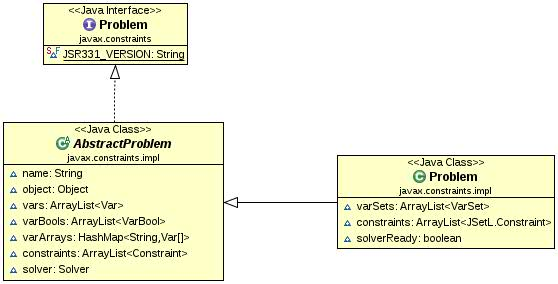
\includegraphics[scale=.5]{img/Problem.JPG}
\caption{Class Diagram di \texttt{Problem}.}
\end{figure}

\subsection{Implementazione}
Una volta definita la classe, come visto all'inizio 
della sezione \ref{problem}, sono stati inseriti tutti i metodi astratti
dell'interfaccia \files{Problem} non definiti nell'implementazione di base. 

Si descrivono ora gli attributi ed i metodi definiti, basati sul solver JSetL.

\subsubsection{Attributi}
Come accennato in precedenza, l'implementazione di base fornisce attributi
di classe per la gestione di variabili intere, booleane e per i vincoli, ma
non prevede nulla per quelle insiemistiche. Sono stati quindi aggiunti,
sulla base del medesimo meccanismo di \files{AbstractProblem}, attributi
per la gestione di queste variabili.
\begin{lstlisting}[language = Java,
                   caption = {attributi di \texttt{Problem}.}]
ArrayList<VarSet> varSets;

private static final int OPER_EQ = 1, OPER_UNKNOWN = 0, OPER_NEQ = 2, OPER_LT = 3, OPER_LEQ = 4, OPER_GT = 5, OPER_GEQ = 6;

private static int counter = 0;
\end{lstlisting}
L'attributo
\files{varSets} rappresenta la lista delle variabili insiemistiche appartenenti 
al problema. 

Sono state poi definite delle costanti utili per identificare gli operatori
($=$, $\leq$, $\geq$, $\ldots$) 
mediante il costrutto \files{switch} (che richiede come parametro un intero) e
delle variabili globali utilizzate per contare variabili interne al fine di 
assegnare un nome univoco alle stesse.

\subsubsection{Costruttori} 
I costruttori richiesti sono due: uno senza parametro ed uno con parametro
\files{String} che ne rappresenta il nome.
\begin{lstlisting}[language = Java,
                   caption = {costruttore con parametro.}]
public Problem(String name) {
	super(name);
	varSets = new ArrayList<VarSet>();
}
\end{lstlisting}

In entrambi i casi viene chiamato il costruttore della classe astratta di base
con la sola differenza che quello senza parametro assegna un valore di
default al nome:
\begin{lstlisting}[language = Java, frame = single]
	super("_P"+(counter++));
\end{lstlisting} 
e quindi viene inizializzata la lista delle variabili proprie della classe, 
ovvero quelle insiemistiche che si sono ridefinite nella nostra implementazione.

\subsubsection{Metodo \texttt{postElement}}
L'interfaccia \files{Problem} specifica anche metodi  per creare vincoli 
che hanno a che fare con elementi di array di interi o di variabili vincolate
intere. Se una variabile logica intera \files{indexVar} ha la funzione di
indice all'interno di un array \files{v}, il risultato di un'operazione
\files{v[indexvar]} è un'altra variabile vincolata. Poiché Java
non supporta l'overloading dell'operatore ``\files{[]}'' l'interfaccia
standard utilizza questo metodo.

Vi sono quattro possibili definizioni di questo metodo:
\begin{lstlisting}[language = Java, frame = single]
  public Constraint postElement(int[], Var, String, int);
  public Constraint postElement(int[], Var, String, Var);
  public Constraint postElement(Var[], Var, String, int);
  public Constraint postElement(Var[], Var, String, Var);
\end{lstlisting}

Vediamo nel dettaglio solo uno di questi metodi poiché in tutti e quattro i casi
si utilizza la classe di supporto \texttt{Element} che rappresenta il vincolo 
specificato mediante i parametri del costruttore e che sarà definito in 
\ref{Element}.

\begin{lstlisting}[language = Java,
                   caption = {\files{postElement}, array di interi.}]
public Constraint postElement(
                int[] array, 
                javax.constraints.Var indexVar, 
                String oper, 
                int value) {
        if (indexVar.getMin() > array.length - 1 || indexVar.getMax() < 0)
                throw new RuntimeException("elementAt: invalid index variable");
        Element result = new Element(array, indexVar, oper, value);
        post(result);
        return result;
}
\end{lstlisting}
Innanzitutto viene controllato che il dominio della variabile indice sia
compatibile con il range dell'array, altrimenti viene lanciata un'eccezione.
Viene quindi istanziata la variabile \texttt{result} di tipo \texttt{Element}
con i medesimi parametri del metodo invocato. Questa variabile rappresenta il
vincolo:
\begin{center}
\lstinline$array[indexVar] oper value$,
\end{center}
che viene infine aggiunto al problema mediante il metodo \texttt{post}.

\subsubsection{Metodo \texttt{post}}
Un vincolo non ha effetto fino a che non viene inserito nel problema. Per 
fare ciò si utilizza il metodo \files{post}, che ha le seguenti dichiarazioni:
\begin{lstlisting}[language = Java, frame = single]
public Constraint post(int[], Var[], String, int);
public Constraint post(int[], Var[], String, Var);
public Constraint post(Var[], String, int);
public Constraint post(Var[], String, Var);
public Constraint post(Var, String, int);
public Constraint post(Var, String, Var);
public Constraint post(Constraint);
\end{lstlisting}
Ogni metodo \files{post} ha il medesimo approccio: costruisce il vincolo 
basandosi sul metodo \files{linear} (si entrerà
nel dettaglio nei prossimi paragrafi), lo pubblica nel solver JSetL mediante
la chiamata della specifica \files{post(Constraint)} ed infine
lo aggiunge ai vincoli del problema con il metodo \files{add}.

\begin{lstlisting}[language = Java,
                   caption = {\files{post}.},
                   label = codicepost]
public Constraint post(
                int[] array, 
                javax.constraints.Var[] vars, 
                String oper, 
                int value) {
        Constraint result = linear(array, vars, oper, value);
        post(result);
        add(result);
        return result;
}

public Constraint post(
                Var var, 
                String oper, 
                int value) {
	Constraint result = linear(var, oper, value);
	post(result);
	add(result);
	return result;
}
\end{lstlisting}
Nel listato \ref{codicepost} si possono notare due metodi \files{post} 
standard, uno per le 
variabili singole (il secondo) ed uno per array di variabili. Entrambi 
utilizzano il metodo \files{linear} e restituiscono il nuovo vincolo
creato. 

\begin{lstlisting}[language = Java,
                   caption = {\files{post(Constraint)}.}]
public void post(javax.constraints.Constraint constraint) {
        add(constraint);
        addJSetLConstraints((JSetL.Constraint) constraint.getImpl());
}
\end{lstlisting}
Questo è invece il metodo su cui tutti gli altri si basano per aggiungere
il vincolo creato al \texttt{Problem}. Viene invocata la funzione \texttt{add}
della classe base per aggiungere il vincolo JSR-331. Quindi mediante il
metodo \texttt{addJSetLConstraints} si inserisce il vincolo specifico di
JSetL all'array di supporto.
\begin{flushleft}
Anche la classe \files{Constraint} ha un metodo \files{post}, per cui è 
possibile creare un vincolo e quindi renderlo attivo con la seguente sintassi:
\begin{lstlisting}[language = Java, frame = single]
Constraint c = p.linear(x, ``<='', y);
c.post();
\end{lstlisting}
\end{flushleft}

\subsubsection{Metodi \texttt{linear}}\label{metLinear}
I vincoli che hanno a che fare con il confronto di espressioni vincolate
utilizzano gli operatori di confronto standard:
\[
\begin{array}{c|c}
\textbf{Stringa} & \textbf{Semantica} \\
\hline \hline
< & \textrm{minore stretto,} \\
<= & \textrm{minore o uguale,} \\
= & \textrm{uguale,} \\
>= & \textrm{maggiore o uguale,} \\
> & \textrm{maggiore stretto,} \\
!= & \textrm{diverso.} \\
\end{array}
\]

I metodi che implementano il confronto sono chiamati \files{linear} e vengono
usati, come accennato in precedenza, nelle definizioni di \files{post}. \`E
anche possibile per l'utente utilizzare direttamente \files{linear}, non sono 
infatti
metodi privati, e sono utili perché non aggiungono direttamente un vincolo
e le variabili al problema.

Vi sono quattro differenti metodi \files{linear}:
\begin{lstlisting}[language = Java, frame = single]
public Constraint linear(int[], Var[], String, int);
public Constraint linear(int[], Var[], String, Var);
public Constraint linear(Var, String, int);
public Constraint linear(Var, String, Var);
\end{lstlisting}
i primi due hanno a che fare con vettori di variabili vincolate, mentre gli 
altri ne gestiscono una sola. In entrambi i casi si effettua il confronto
con un intero o un'altra variabile vincolata.

\begin{lstlisting}[language = Java,
                   caption = {\files{linear}, con array di variabili.}]
public Constraint linear(
                int[] array, 
                javax.constraints.Var[] vars, 
                String oper, int value) {
        if (array.length != vars.length || array.length == 0)
                throw new RuntimeException(
                        "Coefficent and variable length must be equal and not zero.");
        Var scalprod = (Var) scalProd(array, vars);
        return new Linear(scalprod, oper, value);
}
\end{lstlisting}
Il metodo con i vettori, dopo aver verificato che le lunghezze siano 
compatibili e non nulle, genera il prodotto scalare tra i due array tale che
se $v_0, v_1, \ldots, v_{n-1}$ sono le variabili contenute in \files{vars} e
$a_0, a_1, \ldots, a_{n-1}$ sono i coefficienti interi contenuti in 
\files{array},
la variabile vincolata $s$ rappresentata da \files{scalprod} è data da:
\[
s = a_0\cdot v_0 + a_1\cdot v_1 + \cdots + a_{n-1}\cdot v_{n-1}.
\]

Una volta creata la variabile temporanea \files{scalprod} viene calcolato 
e ritornato il vincolo mediante il costruttore della classe \texttt{Linear}.

\begin{lstlisting}[language = Java,
                   caption = {\files{linear}, con variabile singola.}]
public Constraint linear(
                javax.constraints.Var var, 
                String oper, 
                int value) {
        if (var == null)
                throw new RuntimeException("Parameters must not be null.");
        return new Linear(var, oper, value);
}
\end{lstlisting}
Nel metodo con la singola variabile viene controllato che \files{var} non sia
nulla, nel qual caso viene lanciata un'eccezione, anche quindi viene ritornata
la costruzione di un nuovo vincolo specifico di tipo \texttt{Linear}, discusso
nella sezione \ref{Linear}.

\subsubsection{Metodo \texttt{scalProd}}
Questo metodo pubblico permette di creare una nuova variabile vincolata
intera che rappresenta il prodotto scalare tra gli elementi degli array
passati come parametro. Come si è già visto per il metodo \files{linear} il
risultato che si ottiene è del tipo:
\[
s = a_0\cdot v_0 + a_1\cdot v_1 + \cdots + a_{n-1}\cdot v_{n-1}.
\]

\files{scalProd} è spesso utilizzato all'interno di altri metodi, ma è comunque
definito pubblicamente poiché rappresenta un'operazione comune per le variabili.

\begin{lstlisting}[language = Java,
                   caption = {\files{scalProd}.}]
public Var scalProd(int[] values, Var[] vars) {
  .
  .
  IntLVar[] intVars = new IntLVar[vars.length];
  if (values[0] != 0)
    intVars[0] = ((Var) vars[0]).getIntLVar().mul(values[0]);
  else intVars[0] = new IntLVar(0,0);
  for (int i = 1; i < values.length; i++) {
    if (values[i] !=0) {
      IntLVar tmp = new IntLVar(((Var) vars[i]).getIntLVar().mul(values[i]));
      intVars[i] = intVars[i-1].sum(tmp);
    }
    else intVars[i] = intVars[i-1];
  }
  return new Var(this, intVars[vars.length-1]);
}
\end{lstlisting}
Inizialmente il metodo controlla le lunghezze degli array (parte omessa) e se
non compatibili o se nulli lancia una \texttt{Runtime Exception}.

Quindi viene creato un array ausiliario di \files{IntLVar} di lunghezza pari
a quella dei due vettori \files{vars} e \files{values}. Questo vettore viene
utilizzato per calcolare i risultati parziali, ovvero nell'$i$-esimo elemento
è contenuto il prodotto scalare dei primi $i+1$ elementi.
\[
\begin{array}{rcl}
\files{vars} & = & [v_0, v_1, \ldots, v_i, \ldots, v_{n-1}] \\
\files{values} & = &  [a_0, a_1, \ldots, a_i, \ldots, a_{n-1}] \\
\hline
\hline
\files{intVars[i]} & = & a_0\cdot v_0 + a_1\cdot v_1 + \cdots + a_i\cdot v_i
\end{array}
\] 

Alla fine del processo si ottiene un array il cui ultimo elemento rappresenta
proprio il prodotto scalare dei due vettori passati come parametro.
A questo punto viene creata e restituita una nuova variabile intera JSR-331
mediante un opportuno costruttore.

\subsubsection{Metodo \texttt{allDifferent}}
L'interfaccia \files{Problem} definisce un modo semplice per creare ed inserire
nel problema uno dei più comuni vincoli globali conosciuto come AllDifferent:
\begin{center}
\lstinline[language = Java]$public Constraint postAllDifferent(Var[] vars);$
\end{center}
\`E definito un altro sinonimo più compatto:
\begin{center}
\lstinline[language = Java]$public Constraint postAllDiff(Var[] vars);$
\end{center}
Questi metodi creano, inseriscono nel problema e restituiscono un nuovo vincolo
per cui ogni variabile dell'array \files{vars} debba avere un valore diverso 
dalle altre.
La definizione del metodo è la seguente:
\begin{lstlisting}[language = Java,
                   caption = {\files{allDifferent}.}]
public Constraint postAllDifferent(Var[] vars) {
	if (vars.length == 0)
		throw new RuntimeException("Variable array must not be empty.");
	Constraint result = new AllDifferent(vars);
	post(result);
	return result;
}
\end{lstlisting}
Questo metodo crea semplicemente un nuovo vincolo appoggiandosi al costruttore 
della classe \files{AllDifferent} che verrà definito nella sezione 
\ref{AllDifferent}.

\subsubsection{Metodi \texttt{postCardinality}}
La specifica JSR-331 include tra i metodi pubblici alcune funzioni che
creano vincoli inerenti alla cardinalità di array di variabili
intere. Questi vincoli detti di cardinalità (\texttt{Cardinality Constraints}), 
che tuttavia non hanno nulla a che fare con le variabili insiemistiche, sono
quattro:
\begin{lstlisting}[language = Java, frame = single]
public Constraint postCardinality(Var[], int, String, int);
public Constraint postCardinality(Var[], int, String, Var);
public Constraint postCardinality(Var[], Var, String, int);
public Constraint postCardinality(Var[], Var, String, Var);
\end{lstlisting}

Poiché sono vincoli abbastanza particolari, la loro trattazione più dettagliata
viene fatta a parte, nella sezione \ref{Cardinality} per quanto riguarda la
classe \texttt{Cardinality} e nell'appendice \ref{cardinality} per l'approccio
e la trattazione del problema d'implementazione di tale vincolo.

\subsubsection{Metodi \texttt{postGlobalCardinality}}
L'interfaccia \files{Problem} specifica anche metodi utili per creare vincoli
di cardinalità globale noti come \emph{GCC} (\emph{Global Cardinality 
Constraints}) che rappresentano non uno, ma più
vincoli di cardinalità allo stesso tempo. La specifica prevede che il livello
d'implementazione di questi possa essere comune o specifico, ovvero è 
fornita un'implementazione nella classe \files{AbstractProblem}. \`E quindi
possibile implementare o meno questi metodi. 

La lista dei metodi, limitata alle variabili intere è la seguente:
\begin{lstlisting}[language = Java, frame = single]
public Constraint postGlobalCardinality(Var[], int[], Var[]);
public Constraint postGlobalCardinality(Var[], int[], int[], int[]);
\end{lstlisting}

In entrambi i casi il metodo sfrutta la costruzione di un vincolo
specifico implementato mediante la classe \texttt{GlobalCardinality} che verrà
definito in \ref{GlobalCardinality}.

\begin{lstlisting}[language = Java,
                   caption = {\files{postGlobalcardinality}.}]
public Constraint postGlobalCardinality(
                Var[] vars, 
                int[] values, 
                Var[] cardinalityVars) {
        Constraint c = new GlobalCardinality(vars, values, cardinalityVars);
        c.post();
        return c;
}
\end{lstlisting}
In questo esempio si può notare che il costruttore utilizza esattamente i 
parametri d'invocazione della funzione. Il vincolo creato viene quindi inserito
nel problema.

\section{Interfaccia comune: \texttt{CommonBase}}\label{common}
Prima di parlare nello specifico delle componenti del problema (inteso come CSP)
e quindi di variabili e vincoli, occorre parlare dell'interfaccia comune.
Come per l'interfaccia \files{Problem} anche le interfacce \files{Var},
\files{VarBool}, \files{VarSet} e \files{Constraint} sono fornite di
un'implementazione astratta (non pura) che fornisce attributi, costrutti e 
metodi di base. Questa è la classe \files{CommonBase}.

\subsection{Attributi}
Gli attributi della classe \files{CommonBase} sono quattro:
\begin{lstlisting}[language = Java, frame = single]
	Problem problem;
	String  name;
	Object  impl;
	Object  businessObject;
\end{lstlisting}
L'attributo
\files{problem} rappresenta il problema a cui l'oggetto del CSP è associato,
la stringa \files{name} è il nome dato all'oggetto. Si parla di oggetto
perché questa classe implementa gli attributi di base di ogni oggetto di un
CSP, ed è chiaro che ogni variabile intera, booleana o insiemistica possa avere
un nome, e \emph{debba} sicuramente avere un problema associato e una
parte implementativa.

La parte implementativa è rappresentata dall'attributo \files{impl}, che per
l'appunto è un'istanza \files{Object}, ovvero l'oggetto generico Java. Ogni
implementazione specifica (come JSetL) deve, se supportato, appoggiarsi
all'attributo \files{impl} per sfruttare la propria implementazione.

L'ultimo attributo della classe è \files{businessObject}, che può essere
utilizzato come attributo di supporto per le specifiche implementazioni.

\subsection{Costruttori}
Con la classe \files{CommonBase} vengono forniti due costruttori, uno senza 
parametro ed uno con parametro stringa che ne rappresenta il nome.
\begin{lstlisting}[language = Java,
                   caption = {costruttori di \files{CommonBase}.},
                   label = list01]
public CommonBase(Problem problem) {
	this(problem,"");
}

public CommonBase(Problem problem, String name) {
	this.problem = problem;
	this.name = name;
	impl = null;
	businessObject = null;
}
\end{lstlisting}
Il primo costruttore definito nel listato \ref{list01} si limita a chiamare il 
secondo passando come parametro la stringa vuota. Quest'ultimo imposta il
problema ed il nome passati come parametro ai relativi attributi \files{problem}
e \files{name}, infine \files{impl} e \files{businessObject} vengono impostati
a \files{null}.

L'importanza di questi costruttori è dovuta al fatto che ogni classe derivata
dalla suddetta dovrà utilizzarli. Questo implica che ogni classe
(\files{Var}, \files{VarBool}, \files{VarSet} e
\files{Constraint}) dovrà fornire tali costruttori di base ed 
utilizzare quindi il metodo \files{setImpl} per definire la propria
implementazione dell'oggetto costruito.  


\subsection{Metodi}
La classe \files{CommonBase} fornisce alcuni metodi comuni per qualsiasi tipo
di variabile o vincolo. Se ne descrivono brevemente alcuni.
\begin{itemize}
\item[-]\lstinline[language = Java]$public Problem getProblem()$

Restituisce il problema a cui l'oggetto
d'invocazione è legato.

\item[-]\lstinline[language = Java]$public void setName(String name)$

Imposta il nome dell'oggetto.

\item[-]\lstinline[language = Java]$public String getName()$

Restituisce il nome dell'oggetto
d'invocazione.

\item[-]\lstinline[language = Java]$public void setImpl(Object impl)$

Imposta l'implementazione concreta di uno 
specifico solver per l'oggetto d'invocazione.

\item[-]\lstinline[language = Java]$public Object getImpl()$

Restituisce l'implementazione concreta (dello 
specifico solver) per l'oggetto d'invocazione.

\item[-]\lstinline[language = Java]$public void setObject(Object obj)$

Aggiunge un oggetto ausiliari.

\item[-]\lstinline[language = Java]$public Object getObject()$ 

Restituisce l'oggetto ausiliario.
\end{itemize}


\section{Classe \texttt{Var}}
Questa classe implementa le variabili intere vincolate
\files{Var} per la specifica JSR-331
estendendo la classe \files{AbstractVar} (e quindi 
\files{CommonBase}).

Come visto nella descrizione dell'interfaccia comune vengono forniti tutti gli
attributi e metodi utili ed è quindi sufficiente implementare i metodi
dell'interfaccia \files{AbstractVar} ed i costruttori di \files{CommonBase},
mappando quindi le funzionalità richieste per la classe \files{Var}
con quelle fornite da JSetL (tramite \files{IntLVar}).

\begin{lstlisting}[language = Java,
                   frame = single,
                   caption = {metodi di Var},
                   label = metodiVar]
        public int getMin();
	public int getMax(); 
	public boolean isBound();
	public boolean contains(int value);
	public Var plus(int value);
	public Var minus(int value);
	public Var plus(Var x);
	public Var minus(Var x); 
	public Var multiply(int value);
	public Var multiply(Var x);
	public Var divide(int value);
	public Var divide(Var x);
\end{lstlisting}

\subsection{Costruttori}
Sono stati implementati vari costruttori per la classe \files{Var} atti
a soddisfare diverse esigenze, in primis quelle richieste dalla specifica e 
quindi altre suggerite dallo sviluppo del progetto.

Il meccanismo è simile per tutti i costruttori: si richiama il costruttore
della classe base (mediante il costrutto \files{super}) con il
parametro \files{Problem} (e a volte il nome), quindi si imposta l'oggetto
\files{impl} con l'implementazione concreta.
 
\begin{lstlisting}[language = Java,
                   caption = {un costruttore di \files{Var}.}]
public Var(Problem problem) {
	super(problem);
	String name = problem.getFreshName();
	setImpl(new IntLVar(name));
	setName(name);
}
\end{lstlisting}
In questo esempio si vede il costruttore con il solo parametro \files{problem}.
Viene chiamato il costruttore \files{AbstractVar(problem)} mediante il
costrutto \files{super(problem)}, quindi viene generato un nuovo nome mediante
la funzione di 
supporto \files{getFreshName}\footnote{\samepage La funzione ausiliaria 
\files{getFreshName} si limita a
creare un nome per le variabili interne che sia unico, al fine di rendere più
chiara la fase di debugging, non è trattata nel dettaglio.} della 
classe \files{Problem}.

A questo punto viene impostato l'attributo \files{impl} con una nuova istanza
della classe \files{IntLVar} creata con il costruttore con parametro stringa,
che ne rappresenta il nome, infine questo
viene settato anche per la variabile \files{Var}.

\begin{figure}[!ht]\label{varUML}
\centering
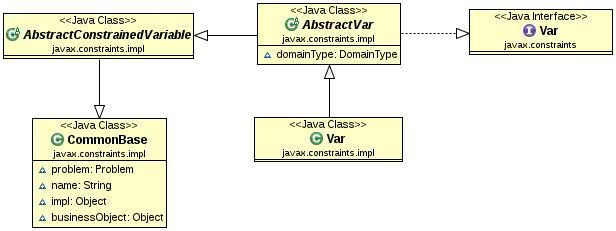
\includegraphics[scale=.5]{img/Var.JPG}
\caption{Class Diagram di \texttt{Var}.}
\end{figure}

\subsection{Metodi di uso generale}
I primi quattro metodi dell'elenco \ref{metodiVar} sono metodi di utilità 
generica e se ne dà una descrizione dettagliata.
\subsubsection{Metodo \texttt{getMin}}
Il metodo \files{getMin} restituisce il più piccolo intero del dominio
della variabile d'invocazione. \`E definito nel seguente modo:
\begin{lstlisting}[language = Java,
                   caption = {\files{getMin}.}]
public int getMin() {
	MultiInterval domain = ((IntLVar) getImpl()).getDomain();
	return domain.getGlb();
}
\end{lstlisting}
Dapprima viene presa l'implementazione concreta con il metodo \files{getImpl},
che in questo caso restituisce l'istanza di \files{IntLVar} relativa alla
variabile d'invocazione (\files{this}). A questo punto, mediante il metodo 
\files{getDomain},
dalla variabile si ottiene il dominio sotto forma di \files{MultiInterval}.
Viene quindi restituito il minimo valore di \files{domain} con il
metodo \files{MultiInterval.getGlb}.

\subsubsection{Metodo \texttt{getMax}}
Il metodo \files{getMax} restituisce il più grande intero del dominio
della variabile d'invocazione. \`E definito nel seguente modo:
\begin{lstlisting}[language = Java,
                   caption = {\files{getMax}.}]
public int getMin() {
	MultiInterval domain = ((IntLVar) getImpl()).getDomain();
	return domain.getGlb();
}
\end{lstlisting}
Analogamente a \files{getMin} questo metodo sfutta le funzionalità di
\files{IntLVar} e \files{MultiInterval}.

\subsubsection{Metodo \texttt{isBound}}
Il metodo \files{isBound}, come suggerisce il nome, è di tipo booleano, ovvero
ha due possibili valori di ritorno: \files{true} se il dominio della variabile
vincolata si riduce ad un singoletto, \files{false} altrimenti.
\begin{lstlisting}[language = Java,
                   caption = {\files{isBound}.}]
public boolean isBound() {
	return ((LVar) getImpl()).isBound();
}
\end{lstlisting}
Questo metodo si appoggia semplicemente al relativo metodo di JSetL per le
variabili intere.

\subsubsection{Metodo \texttt{contains}}
Anche questo è un metodo booleano, restituisce \files{true} se e solo se
un dato intero appartiene al dominio della variabile.
\begin{lstlisting}[language = Java,
                   caption = {\files{contains}.}]
public boolean contains(int value) {
	MultiInterval domain = ((IntLVar) getImpl()).getDomain();
	return domain.contains(value);
}
\end{lstlisting}
Come nei metodi precedenti viene prima richiamato il dominio della variabile
JSetL e in seguito viene ritornato il medesimo metodo sui multi-intervalli
\files{MultiInterval.contains(int)}.

\subsection{Operazioni aritmetiche}
La classe \files{AbstractVar} prevede l'implementazione dei comuni operatori
aritmetici per le variabili intere: ``$+$'', ``$\cdot$'', ``$-$'', ``$\div$''.

Per ogni operatore è definita una funzione con parametro intero ed una che abbia
come parametro un'altra variabile intera, questo permette di ottenere delle
espressioni del tipo:
\[
X + k, \quad X + Y,
\]
dove $X$ e $Y$ rappresentano delle variabili intere vincolate e $k$ un intero.

La lista dei metodi aritmetici è definita dalle ultime otto dichiarazioni
del listato \ref{metodiVar}, poiché si basano tutte sullo stesso principio ne
verranno definite nel dettaglio solo due, una con parametro intero ed
una con parametro variabile.

\begin{lstlisting}[language = Java,
                   caption = {\files{plus}, con parametro intero.}]
public Var plus(int value) {
	Problem p = (Problem) getProblem();
	Var x = new Var(p, p.getFreshName());
	x.setImpl(((IntLVar) getImpl()).sum(value));
	((IntLVar)x.getImpl()).setName(x.getName());
	// To constraint the new variable.
	Constraint c = new Constraint(p,
		((IntLVar) x.getImpl()).eq(((IntLVar) getImpl()).sum(value)));
	p.post(c);
        return x;
}
\end{lstlisting}
Il metodo crea una nuova variabile \files{x} di tipo \files{Var} che
poi verrà restituita come risultato, a questa viene assegnato un nuovo nome
e una nuova implementazione, vincolata ad essere il risultato della somma
della variabile d'invocazione e dell'intero \files{value}.

A questo punto si potrebbe dire che il lavoro sia finito e si possa
restituire il 
risultato, tuttavia si commetterebbe un errore. La nuova variabile deve infatti
essere vincolata ed è quindi necessario aggiungere al
solver JSetL il vincolo $X = T+k$ dove $X$ è la variabile creata, $T$ è
quella di invocazione e $k$ l'intero \files{value}.

Questa aggiunta (che, nel codice, è definita subito dopo il commento) è stata
dovuta non tanto per la correttezza del metodo per quanto riguarda le variabili
del problema, ma per le variabili di supporto i cui vincoli non verrebbero 
aggiornati all'interno del solver JSetL.

\begin{lstlisting}[language = Java,
                   caption = {\files{multiply}, con parametro variabile.}]
public Var multiply(javax.constraints.Var x) {
        Problem p = (Problem) getProblem();
        Var a = new Var(p, p.getFreshName());
        a.setImpl(((IntLVar) getImpl()).mul(((Var) x).getIntLVar()));
        ((IntLVar)a.getImpl()).setName(a.getName());
        // To constraint the new variable.
        Constraint c = new Constraint(p,
             ((IntLVar) a.getImpl()).eq(((IntLVar) getImpl()).mul((IntLVar) x.getImpl())));
        p.post(c);
        return a;
}
\end{lstlisting}
Come si può notare il metodo con parametro variabile è sostanzialmente identico,
l'unica differenza è data dalla chiamata della funzione \files{getImpl}
per il parametro \files{x} all'interno del costruttore del nuovo vincolo
inserito.

\section{Classe \texttt{VarBool}}
La classe \files{VarBool} rappresenta le variabili booleane. Queste si 
possono considerare un caso particolare 
delle variabili intere, con il dominio ristretto ai valori $[0,1]$. In cui
$0$ rappresenta il valore \files{false} e $1$ il valore \files{true}.

JSR-331 fornisce un'implementazione di base per questa classe che estende
\files{Var}, tuttavia si è scelto di ridefinirla (anche se in modo del tutto
analogo) per avere una gestione più diretta e per facilitare eventuali
modifiche future.
\begin{lstlisting}[language = Java, frame = single]
public class VarBool extends Var implements VarBool {
\end{lstlisting}
\subsection{Costruttori}
I costruttori della classe chiamano quelli della classe base
\files{Var} e quindi impostano l'implementazione con una variabile dal
dominio $[0,1]$
\begin{lstlisting}[language = Java,
                   caption = {un costruttore di \files{VarBool}}]
public VarBool(Problem problem, String name) {
	super(problem, name);
	setImpl(new IntLVar(name, 0, 1));
}
\end{lstlisting}

\section{Classe \texttt{VarSet}}
La specifica JSR-331 introduce un'interfaccia basilare per le variabili
insiemistiche vincolate. Al contrario delle variabili intere, quando un'istanza
 di questa classe è considerata bound  significa che coincide ad un 
singolo insieme di
valori interi.

Il pacchetto \files{javax.constraints.impl} fornisce la classe 
\files{BasicVarSet} che di fatto implementa l'interfaccia \files{VarSet}. 
Tuttavia poiché JSetL ha le proprie classi che implementano insiemi, 
e soprattutto insiemi di interi mediante la classe \files{SetLVar}, si è deciso
di non considerare l'implementazione di base fornita e proseguire con 
l'approccio utilizzato per la classe \files{Var}.
\begin{lstlisting}[language = Java,
                   frame = single]
public class VarSet extends AbstractConstrainedVariable 
    implements javax.constraints.VarSet {
\end{lstlisting}

La classe estende \files{AbstractConstrainedVariable} e quindi 
\texttt{CommonBase}  che come si è già più volte
sottolineato, fornisce tutti gli strumenti necessari. Inoltre 
\files{VarSet} implementa direttamente l'interfaccia \files{VarSet}, al
contrario di quanto visto per la classe \texttt{Var}.


\begin{figure}[!ht]\label{varsetUML}
\centering
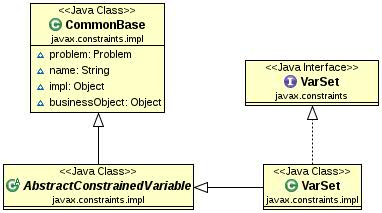
\includegraphics[scale=.75]{img/VarSet.JPG}
\caption{Class Diagram di \texttt{VarSet}.}
\end{figure}

\begin{flushleft}
Il dominio di una variabile insiemistica consiste in due insiemi:
\begin{enumerate}
\item[-]Required Set: un insieme di interi i cui valori appartengono
 tutti alla variabile (lower bound);
\item[-]Possibile Set: un insieme di interi in cui almeno un valore
appartiene alla variabile (upper bound).
\end{enumerate}
\end{flushleft}
Il Required Set è sempre un sottoinsieme del Possibile Set. Ad esempio,
se una variabile insiemistica rappresenta i giorni lavorativi della settimana, 
i valori possibili sono: $\{1, 2, 3, 4, 5, 6, 7 \}$, mentre quelli richiesti
dovranno essere un sottoinsieme di cardinalità $5$, ad esempio 
$\{1, 2, 3, 4, 5\}$. 
\`E permesso rimuovere elementi solo dai valori possibili ed
aggiungerli solo a quelli richiesti. La cardinalità di una variabile
insiemistica vincolata è una variabile intera vincolata. \`E possibile definire
intersezione ed unione di variabili insiemistiche.


Se chiamiamo $V$ una generica variabile insiemistica, $L$ e $U$ due insiemi di
interi che rappresentano rispettivamente Required Set e Possibile Set,
tale che $L \subseteq U$, allora il dominio di $V$ si può esprimere nel
seguente modo:
\[
\textrm{dom}(V) = \{L,U\}.
\]
\begin{flushleft}
Tutte queste caratteristiche, specificate nel documento di riferimento di
JSR-331 \cite{specifiche}, sono già presenti nella classe \files{SetLVar} di 
JSetL, ed è
stato quindi semplice e naturale sfruttarne le caratteristiche.
\end{flushleft}
\subsection{Costruttori}
I costruttori richiesti dall'interfaccia sono solo quelli definiti in
\files{CommonBase}, infatti \files{VarSet} non ne prevede dei propri. I 
costruttori standard sono:
\begin{lstlisting}[language = Java,
                   frame = single]
public VarSet(Problem);
public VarSet(Problem, String);
\end{lstlisting}
mentre quelli definiti in un secondo momento, per venire incontro alle 
necessità implementative sono:
\begin{lstlisting}[language = Java,
                   frame = single]
public VarSet(Problem,  int[], String);
public VarSet(Problem, Set<Integer>, Set<Integer>, String);
public VarSet(Problem, MultiInterval, String);
public VarSet(Problem, SetLVar);
\end{lstlisting}

Come per la classe \files{Var} ogni costruttore utilizza il medesimo
approccio: viene chiamato il costruttore della classe base  mediante il 
costrutto
\files{super} e quindi viene impostato l'oggetto \files{impl} con
una chiama al relativo costruttore di \files{SetLVar}.

Si danno alcuni esempi.

\begin{lstlisting}[language = Java,
                   caption = {un costruttore standard di \files{VarSet}}]
public VarSet(Problem problem, String name) {
	super(problem);
	setImpl(new SetLVar(name));
	setName(name);
}
\end{lstlisting}
Il costruttore in questione si comporta esattamente come quello definito per
la classe \files{Var}.

\begin{lstlisting}[language = Java,
                   caption = {costruttore con lista di interi.}]
public VarSet(Problem problem,  int[] values, String name) {
	super(problem, name);
	MultiInterval s = new MultiInterval();
	for (int i = 0; i < values.length; i++)
		s.add(values[i]);
	setImpl(new SetLVar(name,s));
}
\end{lstlisting}
In questo costruttore, che ha come parametro una lista di interi ed il nome,
viene creato un multi-intervallo a cui vengono aggiunti uno ad uno tutti gli
elementi dell'array \files{values}. Quindi viene chiamato il costruttore
che ha come parametro un \files{MultiInterval} fornito da JSetL.


\begin{lstlisting}[language = Java,
                   caption = {costruttore con un multi-intervallo.}]
public VarSet(Problem problem, MultiInterval lb, String name) {
	super(problem, name);
	setImpl(new SetLVar(name, lb, MultiInterval.universe()));
}
\end{lstlisting}
Questo costruttore ausiliario sfrutta la classe JSetL \files{MultiInterval}
di cui si è già spesso parlato e che è definita in \cite{tesiAmadini}. 
In questo caso
viene chiamato un costruttore di \files{SetLVar} che utilizza due 
multi-intervalli, il primo rappresenta i valori opzionali, mentre
il secondo quelli richiesti.

Sia $L$ l'insieme che rappresenta il multi-intervallo \files{lb}, $\mathcal{U}$
l'insieme universo (di tutti gli interi rapprensentabili dall'implementazione),
allora la variabile insiemistica creata $V$ ha dominio:
\[
\textrm{dom}(V) = \{ L, \mathcal{U} \}.
\] 

\subsection{Metodi di uso generale}
L'interfaccia \files{VarSet} prevede alcuni metodi di utilità generica, tra cui
si evidenziano:
\begin{lstlisting}[language = Java,frame = single]
public boolean isBound();
public Set<Integer> getValue() throws Exception;
public void setValue(Set<Integer> set) throws Exception;
public Set<Integer> getRequiredSet();
public Set<Integer> getPossibleSet();
public boolean isPossible(int value);
public boolean isRequired(int value);
public void remove(int value) throws Exception;
public void require(int val) throws Exception;
public boolean contains(Set<Integer> setOfValues);
public void setEmpty(boolean flag);
public Var getCardinality();
\end{lstlisting}
Alcuni di questi metodi si avvalgono della controparte nell'implementazione
concreta  JSetL e quindi non se ne darà la definizione. Tra questi
si ha \files{isBound}, \files{getValue} e \files{setValue}.

I metodi che hanno a che fare con il dominio invece seguono un altro approccio,
dovendosi basare sulla funzione \files{getDomain} che restituisce il
dominio della variabile JSetL \files{SetLVar}. Questo dominio è
un'istanza della classe \files{SetInterval} e quindi i metodi sono basati su
questa classe oltre che sui multi-intervalli già citati.

\begin{lstlisting}[language = Java,
                   caption = {metodi getter per il dominio.}]
public Set<Integer> getRequiredSet() {
	return ((SetLVar) getImpl()).getDomain().getGlb();
}

public Set<Integer> getPossibleSet() {
	return ((SetLVar) getImpl()).getDomain().getLub();
}
\end{lstlisting}
Come anticipato la chiave dei metodi \files{getRequiredSet} e 
\files{getPossibleSet} è una funzione della classe
\files{SetInterval} che rappresenta il dominio di una variabile insiemistica.
Con \files{getGlb} viene restituito un multi-intervallo (che implementa un
\files{Set<Integer>}) rappresentante il lower-bound della variabile.
Invece \files{getLub} restituisce l'upper-bound. I due oggetti
mappano perfettamente l'insieme required e possible definiti in \files{VarSet}.

\begin{lstlisting}[language = Java,
                   caption = {un intero è possibile o richiesto?.}]
public boolean isPossible(int value) {
	return ((SetLVar) getImpl()).getDomain().getLub().contains(value);
}

public boolean isRequired(int value) {
	return ((SetLVar) getImpl()).getDomain().getGlb().contains(value);
}
\end{lstlisting}
Nelle funzioni \files{isPossible} e \files{isRequired}, dopo aver ottenuto 
l'insieme required o possible viene utilizzato
 il metodo \files{contains} che restituisce un booleano a seconda che
l'intero passato come parametro sia contenuto nel multi-intervallo di 
invocazione o meno.

\begin{lstlisting}[language = Java,
                   caption = {inserire e rimuovere elementi.}]
public void remove(int value) throws Exception {
	((SetLVar) getImpl()).getDomain().getLub().remove(value);	
}

public void require(int value) throws Exception {
	((SetLVar) getImpl()).getDomain().getGlb().add(value);	
}
\end{lstlisting}
Nella descrizione inziale della classe si è detto che è 
permesso rimuovere elementi solo dai valori possibili ed aggiungerli solo a
quelli richiesti. I metodi \files{remove} e \files{require} implementano 
quanto detto, non sono
state quindi fornite funzioni che aggiungano elementi all'upper-bound
o ne rimuovano dal lower-bound.

\begin{lstlisting}[language = Java,
                   caption = {inclusione insiemistica.}]
public boolean contains(Set<Integer> setOfValues) {
	return ((SetLVar) getImpl()).getDomain().getLub().containsAll(setOfValues);
}
\end{lstlisting}
Il metodo booleano \files{contains} controlla se ogni elemento dell'insieme
dato sia contenuto nel dominio della variabile d'invocazione. 
Utilizza il metodo \files{containsAll} sui multi-intervalli.

\begin{lstlisting}[language = Java,
                   caption = {getter per la cardinalità.}]
public Var getCardinality() {
	Var result = new Var((Problem) getProblem(), ((SetLVar) getImpl()).card());
	return result;
}
\end{lstlisting}
Il metodo \files{getCardinality} si avvale del metodo \files{card} presente 
nella  classe \files{SetLVar}, che
restituisce una variabile vincolata intera rappresentante la cardinalità 
dell'insieme. Questa variabile viene poi utilizzata per costruire una nuova
variabile intera \files{Var}  che viene quindi
restituita dal metodo.

\subsection{Operazioni insiemistiche}
\files{VarSet} prevede le operazioni insiemistiche di unione ed intersezione.
Queste operazioni sono già presenti in \files{SetLVar} ed è stato quindi 
semplice implementarle. JSetL prevede inoltre le operazioni di complementazione
e differenza insiemistica al contrario dello standard, tuttavia non è stata
fornita una implementazione per queste.

\begin{lstlisting}[language = Java,
                   caption = {unione insiemistica.}]
public VarSet union(javax.constraints.VarSet varSet) {
        Problem p = (Problem) getProblem();
        SetLVar tmp = ((SetLVar) varSet.getImpl());
        VarSet result = new VarSet(p);
        result.setImpl(((SetLVar)getImpl()).union(tmp));
        // To constraint the new variable.
        Constraint c = new Constraint(p,
                ((SetLVar) result.getImpl()).eq(((SetLVar)getImpl()).union(tmp)));
        p.post(c);
        return result;
}
\end{lstlisting}

\begin{lstlisting}[language = Java,
                   caption = {intersezione insiemistica.}]
public VarSet intersection(javax.constraints.VarSet varSet) {
        Problem p = (Problem) getProblem();
        SetLVar tmp = ((SetLVar) varSet.getImpl());
        VarSet result = new VarSet(p);
        result.setImpl(((SetLVar)this.getImpl()).intersect(tmp));
        // To constraint the new variable.
        Constraint c = new Constraint(p, ((SetLVar) result.getImpl()).eq(
                        ((SetLVar)getImpl()).intersect(tmp)));
        p.post(c);
        return result;
}
\end{lstlisting}
In entrambi i metodi si dichiara una variabile temporanea di tipo 
\files{SetLVar} che rappresenti la variabile passata come parametro e quindi si 
crea la variabile di tipo \files{VarSet} che diventerà il risultato 
dell'operazione. A \files{result} viene assegnato il risultato
dell'operazione tra la variabile temporanea e la variabile d'invocazione 
concreta. Anche in questo caso, come per le operazioni aritmetiche sulle
variabili intere, occorre aggiornare i vincoli per la nuova variabile creata.
Il sistema utilizzato è quindi il medesimo.


\section{Classe \texttt{Constraint}}\label{constraint}
L'ultima classe che si tratta a riguardo della definizione del problema è
quella che rappresenta il vincolo generico. JSR-331 specifica i vincoli più
comuni che definiscono relazioni tra variabili. Questi vincoli
possono essere ottenuti tramite l'interfaccia \files{Problem} ed ognuno di
essi è un' istanza di questa classe.

\subsection{Implementazione}
\files{Constraint} implementa i vincoli JSR-331 estendendo la classe
astratta dell'implementazione.
\begin{lstlisting}[language = Java,frame = single]
abstract public class AbstractConstraint extends CommonBase implements javax.constraints.Constraint {
\end{lstlisting}
Come si può vedere \files{AbstractConstraint} a sua volta estende 
\files{CommonBase}, già descritta nella sezione \ref{common}. Questo vuol dire 
che ogni attributo e metodo utile è ereditato dalla classe e verrà quindi 
sfruttato nell'implementazione. Si hanno poi i metodi definiti nella classe 
astratta: \files{post},  \files{and},  \files{or},  \files{negation} e
 \files{implies}; a parte il primo sono tutti stati ridefiniti poiché JSetL
fornisce la propria implementazione.

\subsection{Costruttori}
Analogamente a quanto visto per gli altri elementi del problema (le variabili)
i costruttori di questa classe richiedono come parametro il problema.
Viene poi fornito un costruttore che aggiunge il nome ed infine uno ausiliario
per l'implementazione JSetL.

\begin{lstlisting}[language = Java,
                   caption = {i costruttori.}]
public Constraint(Problem problem) {
	super(problem);
	setImpl(new JSetL.Constraint());
}

public Constraint(Problem problem, String name) {
	super(problem, name);
	setImpl(new JSetL.Constraint());
}

public Constraint(Problem problem, JSetL.Constraint constraint) {
	super(problem);
	setImpl(constraint);
}
\end{lstlisting}
I tre costruttori sopra definiti utilizzano il medesimo approccio di ogni
classe che si basa su \files{CommonBase}: chiamano il costruttore base e
quindi impostano l'implementazione concreta di JSetL.

\subsection{Vincoli logici}
La specifica JSR-331 prevede quattro metodi che rappresentano i comuni
operatori logici per creare vincoli: $\wedge$, $\vee$, $\neg$ e $\Rightarrow$.

Siano $\mathcal{C}_1$ e $\mathcal{C}_2$ generici vincoli, allora le seguenti
espressioni sono a loro volta vincoli:
\begin{center}
$\mathcal{C}_1 \wedge \mathcal{C}_2$,\quad
$\mathcal{C}_1 \vee \mathcal{C}_2$, \quad
$\neg \mathcal{C}_1$, \quad
$\mathcal{C}_1 \Rightarrow \mathcal{C}_2$.
\end{center}

\subsubsection{Congiunzione logica}
La congiunzione logica è implementata tramite il metodo \files{and} ed ha un
parametro di tipo \files{Constraint}:
\begin{lstlisting}[language = Java,
                   caption = {\files{and}.}]
public Constraint and(Constraint c) {
	JSetL.Constraint constraint = ((Constraint) c).getConstraint();
	Constraint result = new Constraint(getProblem(), this.getConstraint().and(constraint));
	return result;
}
\end{lstlisting}
Il metodo semplicemente crea un nuovo vincolo mediante il costruttore ausiliario
creato per JSetL. Utilizza il metodo \files{and} della classe
\files{Constraint} di JSetL.

\subsubsection{Disgiunzione logica}
Anche la disgiunzione logica ha un vincolo come parametro ed è implementata 
dal seguente codice: 
\begin{lstlisting}[language = Java,
                   caption = {\files{or}.}]
public Constraint or(Constraint c) {
	JSetL.Constraint constraint = ((Constraint) c).getConstraint();
	Constraint result = new Constraint(getProblem(), this.getConstraint().or(constraint));
	return result;		
}
\end{lstlisting}
Il metodo è praticamente identico al primo, con l'unica differenza che nel
costruttore è utilizzato il metodo \files{or}. 

\subsubsection{Negazione}
La Negazione, contrariamente agli altri metodi, non ha argomenti, per il 
resto è identico come approccio: viene creato un nuovo vincolo
mediante il metodo \files{notTest}:
\begin{lstlisting}[language = Java,
                   caption = {\files{negation}.}]
public Constraint negation() {
	Constraint result = new Constraint(getProblem(), this.getConstraint().notTest());
	return result;		
}
\end{lstlisting}

\subsubsection{Implicazione}
L'implicazione segue di pari passo i primi due metodi descritti: ha un parametro
di tipo \files{Constraint} e crea un nuovo vincolo mediante il metodo
\files{impliesTest} di JSetL.
\begin{lstlisting}[language = Java,
                   caption = {\files{implies}.}]
public Constraint implies(Constraint c) {	
	JSetL.Constraint constraint = ((Constraint) c).getConstraint();
	Constraint result = new Constraint(getProblem(), this.getConstraint().impliesTest(constraint));
	return result;
}
\end{lstlisting}
\begin{nota}
Nella classe \files{JSetL.Constraint} erano presenti i soli metodi \files{or} e
\files{and} che implementavano la disgiunzione e congiunzione logica
(la disgiunzione viene propagata in modo 
non deterministico). Durante lo sviluppo dell'interfaccia per la specifica si
è reso necessaria l'introduzione di metodi per
la negazione e l'implicazione.

Sono stati quindi forniti i metodi \files{impliesTest}, e
\files{notTest} che realizzano un'implementazione deterministica delle
relative operazioni logiche.

Nell'approccio di JSetL per la soluzione dei vincoli il non determinismo 
garantisce il risultato a scapito dell'efficienza; tuttavia sono stati 
introdotti altri sistemi per raggiungere la correttezza e la completezza, come 
il labeling visto nel capitolo \ref{jsetl}.

L'approccio nello sviluppo dell'implementazione JSR-331 basata su JSetL verte 
sul labeling di ogni
variabile inserita nel problema e questo garantisce un risultato quando si
cerca una soluzione. Per questo motivo l'utilizzo di metodi  deterministici
non è un problema, anzi in alcuni test si è rivelato un approccio molto
più efficiente.
\end{nota}

\section{Vincoli specifici}\label{nuoviConstraint}
Durante il testing mediante TCK e con l'esecuzione di alcuni
esempi inclusi nella cartella \files{sample} dello stesso si è resa necessaria
l'implementazione di alcune classi non incluse nel documento di specifica:
\begin{itemize}
  \item[-]\files{AllDifferent.java}
  \item[-]\files{And.java}
  \item[-]\files{Cardinality.java}
  \item[-]\files{Element.java}
  \item[-]\files{GlobalCardinality.java}
  \item[-]\files{IfThen.java}
  \item[-]\files{Linear.java}
  \item[-]\files{Neg.java}
  \item[-]\files{Or.java}
\end{itemize}

Ogniuna di queste estende la classe \files{Constraint} e ne ridefinisce i 
costruttori in modo
tale che rappresenti un ben definito vincolo. Alcune di queste classi sono 
utilizzate
nelle definizioni dei vari metodi della classe \texttt{Problem} per la
creazione e l'inserimento di vincoli relativi al problema, altre invece ne
sfruttano le peculiarità.

Poiché ogni classe che implementa vincoli specifici estende 
\texttt{Constraints} non saranno date tutte le definizioni di classe, se ne
fornisce una a fine esemplificativo:
\begin{lstlisting}[language = Java,frame = single]
public class Linear extends Constraint {
\end{lstlisting}
Verranno quindi di seguito, per ogni vincolo, descritti i costruttori più
significativi.

\subsection{Classe \texttt{Linear}}\label{Linear}
Questa classe rappresenta il più classico vincolo sulle variabili logiche
intere, ovvero il vincolo lineare. JSR-331 prevede quattro possibili
vincoli come descritto nella sezione \ref{metLinear}. 

I costruttori che hanno come parametri array di interi e variabili funzionano
esattamente come il metodo \texttt{scalProd} definito all'interno della
classe \texttt{Problem}. L'unica differenza è che una volta computata la
variabile rappresentante il prodotto scalare questa viene vincolata al valore
o alla variabile passata come parametro mediante l'operatore dato, esattamente
come verrà descritto di seguito.
Non se ne darà quindi una descrizione dettagliata.

Per quanto riguarda i costruttori con variabili singole si dà la definizione
di uno solo dei metodi poiché pressoché identici. Entrambi hanno come primo
parametro una variabile \texttt{var} o \texttt{var1}, come secondo una stringa 
\texttt{oper} e come terzo ed ultimo una variabile \texttt{var2} o un intero
\texttt{value}.
La stringa \files{oper} rappresenta
l'operatore di confronto che viene gestito dalla funzione \files{getOperator},
su cui non ci si soffermerà.

\begin{lstlisting}[language = Java,
                   caption = {costruttore \files{Linear} 
                   con variabile e intero.}]
public Linear(javax.constraints.Var var, String oper, int value) {
        super(var.getProblem());
	IntLVar v = ((Var) var).getIntLVar();
	switch(getOperator(oper)) {
	case 1: {
		// Case = "equals".
		JSetL.Constraint constraint = v.eq(value);
		setImpl(constraint);
	} break;
	case 2: {
		// Case != "not equals".
		JSetL.Constraint constraint = v.neq(value);
		setImpl(constraint);
	} break;
        .
        .
        .
	case 6: {
		// Case >= "greater equals".
		JSetL.Constraint constraint = v.ge(value);
		setImpl(constraint);
	} break;
	default: throw new UnsupportedOperationException();
	}
}
\end{lstlisting}
Inizialmente viene chiamato il costruttore della classe base con l'istanza
della classe \texttt{Problem} della variabile passata come parametro.
Quindi viene estratta la variabile intera JSetL di tipo 
\files{IntLVar} mediante la funzione ausiliaria \files{getIntLVar} (che non
fa altro che chiamare il metodo \files{getImpl} dell'implementazione comune).
Quindi, a seconda del caso, viene creato un vincolo JSetL opportuno 
(nel listato, per leggibilità,
sono stati omessi alcuni casi) utilizzato per essere impostato come
implementazione del vincolo creato mediante il metodo \texttt{setImpl}.
\begin{flushleft}
Ecco un'istruzione JSetL per la creazione del vincolo:
\begin{lstlisting}[language = Java, frame = single]
JSetL.Constraint constraint = v.eq(value);
\end{lstlisting}
\end{flushleft}

Se nessun caso dovesse essere catturato mediante lo \files{switch} 
verrebbe lanciata un'eccezione di operazione non supportata.

Come accennato in precedenza la versione del metodo con due variabili
(\files{var1} e \files{var2}) è di poco differente, infatti inizialmente
viene estratta la seconda variabile JSetL e viene quindi trattata come
quella intera, poiché JSetL fornisce i medesimi metodi per interi e variabili.
Ecco la riga aggiunta prima dello statement \files{switch}:
\begin{lstlisting}[language = Java, frame = single]
IntLVar value = ((Var) var2).getIntLVar();
\end{lstlisting}


\subsection{Classe \texttt{Element}}\label{Element}
\texttt{Element} definisce vincoli per la trattazione di array di variabili
intere o array di variabili logiche intere. JSR-331 richiede
quattro possibili vincoli, poiché simili se ne descriveranno solo due: uno per 
l'array di variabili ed uno per quello di interi.

Di fatto questo è un vincolo lineare che coinvolge gli elementi dell'array
dato, in termini degli indici individuati dal dominio della variabile logica
indice. Ad esempio nel caso:
\begin{center}
\lstinline[language=Java]$Element(int[] array, javax.constraints.Var indexVar, ``='', int value)$
\end{center}
se \texttt{array[indexVar]} è una variabile vincolata che ha come dominio
gli interi del vettore \texttt{array} indicizzati da \texttt{indexVar}, il
vincolo risultante è del tipo:
\begin{center}
\lstinline[language=Java]$array[indexVar] = value$.
\end{center}

I quattro costruttori definiti in questa classe sfruttano tutti la medesima
meccanica per costruire il vincolo, se ne descriverà pertanto solo uno.

\begin{lstlisting}[language = Java,
                   caption = {\texttt{Element} per array di interi.}]
public Element(
                int[] array, 
                javax.constraints.Var indexVar, 
                String oper,
                javax.constraints.Var var) {
        super(indexVar.getProblem());
        if (indexVar.getMin() > array.length - 1 || indexVar.getMax() < 0)
                throw new RuntimeException("elementAt: invalid index variable");
        Problem p = (Problem) var.getProblem();
        JSetL.Constraint element = new JSetL.Constraint();
        IntLVar z = new IntLVar(p.getFreshName());
        IntLVar index = (IntLVar) indexVar.getImpl();
        SolverClass solver = ((Solver) p.getSolver()).getSolverClass();
        ListOps listOps = new ListOps(solver);
        List<Integer> list = new ArrayList<Integer>();
        for (int i = 0; i < array.length; i++)
                list.add(i,array[i]);
        LList l = new LList("array", list);
        element.and(listOps.ithElem(l, index, z));
        if (oper.equals("=")) {
          element.and(z.eq((IntLVar)var.getImpl()));
        .
        .
\end{lstlisting}
Questo costruttore ha come parametro un array di interi, una variabile
logica (\texttt{indexVar}) utilizzata come indice, una stringa rappresentante
la relazione con cui si vuole vincolare la nuova variabile risultante 
\texttt{array[indexVar]} ed infine la variabile vincolante.
L'algoritmo è semplice, viene costruito un nuovo vincolo risultato
\texttt{element} e una variabile ausiliaria \texttt{z} che rappresenta la 
sopracitata variabile \texttt{array[indexVar]}. 
Quindi si sfrutta un vincolo utente JSetL chiamato \texttt{ListOps} che ha come
metodo \texttt{ithElem}, questo implementa esattamente il concetto richiesto,
ovvero data una lista di interi (o variabili) ed un indice $i$, 
vincola una data variabile ad
essere equivalente all'$i$-esimo elemento di tale lista. La variabile in
questione è la nuova variabile ausiliaria. Viene quindi aggiornato il vincolo
\texttt{element} con il vincolo lineare rappresentato dalla stringa 
\texttt{oper} e dalla variabile \texttt{var}. Infine il vincolo creato viene
impostato  nell'implementazione  mediante \texttt{setImpl}.





\subsection{Classe \texttt{Cardinality}}\label{Cardinality}
La classe \texttt{Cardinality} modella il vincolo di cardinalità (vedi appendice
\ref{cardinality} per una trattazione completa), in sintesi
tratta un array di variabili logiche imponendo ad un dato numero di esse il 
soddisfacimento di un vincolo lineare.

La specifica richiede quattro versioni per la classe come visto nella
sezione relativa alle funzioni \texttt{postCardinality} della classe
\texttt{Problem}. Si darà la descrizione di un solo costruttore, poiché 
utilizzano tutti il medesimo approccio, cambiando solo le variabili coinvolte.
\begin{lstlisting}[language = Java,
                   caption = {\texttt{Cardinality}.}]
public Cardinality (Var[] vars, int cardValue, String oper, Var var) {
        super(vars[0].getProblem());
        Problem p = (Problem) vars[0].getProblem();
        IntLVar value = ((javax.constraints.impl.Var) var).getIntLVar();
        JSetL.Constraint cardinality = new JSetL.Constraint();
        IntLVar v = new IntLVar("c"+cardValue, cardValue);
        IntLVar k = new IntLVar("_card"+cardValue);
        SolverClass solver = ((Solver) p.getSolver()).getSolverClass();
        Occurrence listOps = new Occurrence(solver);
        Vector<IntLVar> varsList = new Vector<IntLVar>();
        for (int i = 0; i < vars.length; i++)
                varsList.add((IntLVar) vars[i].getImpl());
        cardinality.and(listOps.occurrence(varsList, v, k));
        switch(p.getOperator(oper)) {
        .
        .
        case 3: {
	     // Case < "less".
	     cardinality.and(k.lt(value));
	}  break;
        .
        .
        Constraint result = new Constraint(p, cardinality);
	((Solver) p.getSolver()).add(result);
	setImpl(result.getImpl());
}
\end{lstlisting}
La costruzione del vincolo di cardinalità si basa su un vincolo JSetL
definito dall'utente\footnote{I vincoli definiti dall'utente in JSetL sono 
trattati in \cite{jsetlMan}.} chiamato \texttt{Occurrence} (vedi 
\ref{occurrence}
per una definizione completa) che di fatto, data una lista di variabili logiche
intere, lega un'altra variabile intera ad
essere il numero di occorrenze degli elementi di tale lista che assumono un 
dato valore.

Ogni costruttore di \texttt{Cardinality} utilizza un'istanza di \texttt{Solver}
poiché i vincoli definiti da utente in JSetL richiedono di essere associati
ad una \texttt{SolverClass}, nel caso di cui sopra la variabile \texttt{solver}.
Altre variabili di supporto sono \texttt{v} e \texttt{k} che rappresentano
rispettivamente il valore a cui le variabili devono equivalere ed il numero
di occorrenze delle variabili nell'array che soddisfano il vincolo di 
equivalenza. 

Operativamente nei costruttori si utilizza un vincolo JSetL 
\texttt{cardinality} che rappresenta la congiunzione dei due vincoli su cui
si basa l'algoritmo. Il primo è un'istanza di \texttt{Occurrence} che vincola
\texttt{k} come scritto sopra, quindi il secondo è un vincolo lineare che
lega la variabile \texttt{k} mediante l'operatore \texttt{oper} al valore
\texttt{value}. Il vincolo lineare è determinato dalla stringa \texttt{oper}
e come per altre funzioni viste in precedenza si utilizza uno \texttt{switch}
ed il metodo \texttt{getOperator} della classe \texttt{Problem}.

Il vincolo JSetL così creato viene quindi utilizzato per impostare 
l'implementazione dell'oggetto \texttt{this}.

\subsection{Classe \texttt{GlobalCardinality}}\label{GlobalCardinality}
JSR-331 specifica due vincoli di cardinalità globale, entrambi
trattano un array di variabili ed utilizzano più vincoli 
\texttt{Cardinality}. Il primo vincola un numero esatto di variabili nell'array
dato, mentre il secondo ne limita il range.
\subsubsection*{Cardinalità esatta}
La prima versione che si presenta è quella con cardinalità esatta, poiché tale
vincolo viene utilizzato in quello con range.
Formalmente il vincolo:
\begin{lstlisting}[language = Java, frame = single]
public GlobalCardinality(Var[] vars, int[] values, Var[] card)
\end{lstlisting}
è tale che, per ogni indice \texttt{i} il numero delle volte in cui il valore
\texttt{values[i]} occorre nell'array \texttt{vars} è \emph{esattamente}
\texttt{card[i]}.
\begin{lstlisting}[language = Java,
                   caption = {corpo del costruttore.}]
        super(vars[0].getProblem());
        if (card.length != values.length) {
                throw new RuntimeException("GlobalCardinality error: arrays values and cardinalityVars do not have same size");
        }
        Problem p = (Problem) vars[0].getProblem();
        Constraint result = new Constraint(p);
        for (int i = 0; i < values.length; i++) {
                Cardinality tmp = new Cardinality(vars, values[i], "=", card[i]);
                result.and(tmp);
        }
        setImpl(result.getImpl());
\end{lstlisting}
Inizialmente il costruttore chiama quello della classe base, quindi verifica che
le dimensioni dei vettori siano compatibili, altrimenti lancia un'eccezione.
Viene creato un vincolo di supporto \texttt{result} che rappresenta la
congiunzione di ogni vincolo di cardinalità coinvolto. Nel ciclo 
\texttt{for} viene creata un'istanza di \texttt{Cardinality} temporanea con gli 
indici relativi come sopra descritto, viene quindi aggiornato \texttt{result}. 
Infine viene impostata l'implementazione del vincolo creato mediante 
\texttt{setImpl}.
\subsubsection*{Cardinalità limitata}
In questa versione il vincolo:
\begin{lstlisting}[language = Java, frame = single]
public GlobalCardinality(Var[] vars, int[] values, int[] cardMin, int[] cardMax)
\end{lstlisting}
è tale che, per ogni indice \texttt{i} il numero delle volte in cui il valore
\texttt{values[i]} occorre nell'array \texttt{vars} è compreso tra
\texttt{cardMin[i]} e \texttt{cardMax[i]} inclusi.

\begin{lstlisting}[language = Java,
                   caption = {inizializzazione delle variabili.}]
        super(vars[0].getProblem());
        Problem p = (Problem) vars[0].getProblem();
        int min = cardMin[0];
        int max = cardMax[0];
        for(int i = 0; i < cardMin.length; i++){
                if(cardMin[i] > cardMax[i]) {
                        throw new RuntimeException("GlobalCardinality error: cardMin["+i+"] <= cardMax["+i+"]");
                }
                if (cardMin[i] < min)
                        min = cardMin[i];
                if (cardMax[i] > max)
                        max = cardMax[i];
        }
        Var[] cardinalityVars = new Var[values.length];
        for (int i = 0; i < cardinalityVars.length; i++) {
                cardinalityVars[i] = new javax.constraints.impl.Var(p, min, max);
                cardinalityVars[i].setName("card"+i);
        }
\end{lstlisting}
Il costruttore chiama quello della classe base, quindi inizializza le variabili
di supporto chiamate \texttt{cardinalityVars} di tipo intero. Queste hanno
tutte un dominio compreso tra il più piccolo degli interi appartenenti all'array
\texttt{cardMin} ed il più grande di \texttt{cardMax}.
\begin{lstlisting}[language = Java,
                   caption = {costruzione del vincolo.}]
        GlobalCardinality result = new GlobalCardinality(vars,values,cardinalityVars);
        for (int i = 0; i < cardinalityVars.length; i++) {
                p.post(cardinalityVars[i],">=",cardMin[i]);
                p.post(cardinalityVars[i],"<=",cardMax[i]);
        }
        setImpl(result.getImpl());
}
\end{lstlisting}
A questo punto viene creato un nuovo vincolo di tipo
\texttt{GlobalCardinality} in cui il vettore di variabili vincolanti 
(\texttt{cardinalityVars}) è costituito da variabili unbound (con dominio 
ristretto per ridurre l'albero delle soluzioni). Ogni elemento di indice
\texttt{i} viene quindi vincolato rispetto ai corrispondenti valori
degli array \texttt{cardMin} e \texttt{cardMax}.

\subsection{Classe \texttt{AllDifferent}}\label{AllDifferent}
Questa classe implementa il famoso vincolo AllDifferent, ovvero dato un array
di variabili logiche, questo impone che ogniuna abbia un valore diverso. 
\begin{lstlisting}[language = Java,
                   caption = {\files{postAllDiff}.}
                  ]
public AllDifferent(javax.constraints.Var[] vars) {
        super(vars[0].getProblem());
        IntLVar[] vec = new IntLVar[vars.length];
        for (int i = 0; i < vars.length; i++)
                vec[i] = ((Var) vars[i]).getIntLVar();
        JSetL.Constraint alldiff = IntLVar.allDifferent(vec);
        setImpl(alldiff);
}
\end{lstlisting}
Il costruttore crea un array di supporto (\files{vec}) di \files{IntLVar} al 
quale
assegna il riferimento alla parte di implementazione concreta dell'array
di variabili intere passate come parametro. Quindi crea un nuovo vincolo JSetL
mediante il metodo \files{allDifferent} della classe \files{IntLVar} che di
fatto vincola ogni variabile ad essere differente dalle altre.

A questo punto viene impostata l'implementazione del vincolo
mediante il solito metodo \texttt{setImpl}.


\subsection{Classi \texttt{And}, \texttt{Or}, \texttt{Neg}, \texttt{IfThen}}
Le classi \texttt{And}, \texttt{Or}, \texttt{Neg} e \texttt{IfThen} 
rappresentano i classici vincoli di congiunzione, disgiunzione, negazione ed
implicazione. La loro trattazione viene fatta in un unico paragrafo poiché
utilizzano lo stesso approccio, ovvero di fatto generano un vincolo
che sfrutta la relativa funzione della classe base. Si da solo la definizione
della classe \texttt{Or} a scopo esemplificativo.
\begin{lstlisting}[language = Java,
                   caption = {Classe \texttt{Or}.}]
public class Or extends Constraint {

    public Or(Constraint c1, Constraint c2) {
            super(c1.getProblem());
            Constraint result = (Constraint) c1.or(c2);
            setImpl(result.getImpl());
    }

}
\end{lstlisting}
Come è evidente dal listato di cui sopra, questo genere di classi è molto
conciso, si limita a definire un costruttore con il numero di parametri pari
a quello della funzione che utilizza per la costruzione del vincolo. 

\begin{figure}[!ht]\label{constraintsUML}
\centering
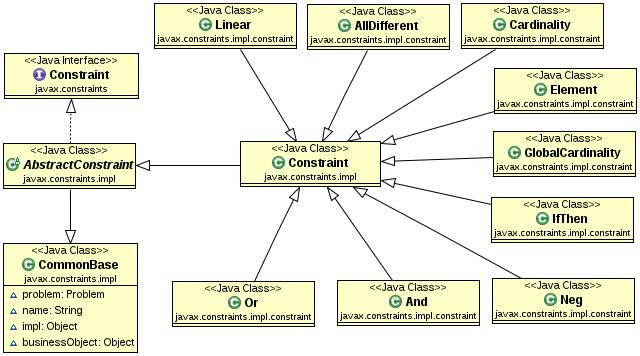
\includegraphics[scale=.5]{img/Constraints.JPG}
\caption{Class Diagram delle classi che implementano i vincoli.}
\end{figure}

\hyphenation{
JSetL
Java
IntLVar
SetLVar
Constraint
JUnit
TCK
}

\chapter{Implementazione: Rappresentazione della Soluzione}\label{capImpl2}
In questo capitolo verranno descritte le classi Java implementate per la
specifica JSR-331 nell'ambito della risoluzione di un problema (CSP).

Per ogni classe descritta verrà introdotta l'interfaccia fornita dalla 
specifica e quindi, con maggior dettaglio, l'implementazione che riguarda
il solver JSetL.


\subsubsection{Risoluzione del problema}
Per rappresentare la risoluzione di un qualsiasi problema, la specifica JSR-331
utilizza le seguenti interfacce: 
\begin{itemize}
\item[-]\files{Solver};
\item[-]\files{SearchStrategy};
\item[-]\files{Solution};
\item[-]\files{SolutionIterator}.
\end{itemize}
Nelle prossime sezioni verranno descritte le suddette classi (implementazioni)
con i principali metodi.


%\section{Risoluzione del problema}
\section{Interfaccia \texttt{Solver}}\label{solver}
Per rappresentare la parte di risoluzione di un qualsiasi CSP, la specifica
JSR-331 utilizza l'interfaccia \files{Solver}. Il solver permette ad un utente
di risolvere un problema cercando una soluzione soddisfacibile od ottimale. Ecco
un esempio:
\begin{lstlisting}[language = Java,
                   caption = {una risoluzione di \files{problem}.}]
        problem.log("=== Find One solution:");
        Solver solver = problem.getSolver();
        Solution solution = solver.findSolution();
        if (solution != null)
          solution.log();
        else
          problem.log("No Solutions");
\end{lstlisting}
In questo semplice esempio il solver cerca una soluzione 
utilizzando una strategia di ricerca di default. La specifica definisce anche 
un'interfaccia per la strategia di ricerca come si vedrà nella sezione
\ref{search}.

\subsection{Come ottenere le soluzioni}
Lo scopo principale dell'interfaccia \files{Solver} è quello di dare all'utente
gli strumenti, dato un problema, per trovarne le soluzioni. Vengono quindi 
forniti i seguenti metodi:
\begin{lstlisting}[language = Java,
                   frame = single]
public Solution findSolution();
public Solution findSolution(ProblemState restoreOrNot);
public Solution findOptimalSolution(Objective objective, Var objectiveVar);
public Solution findOptimalSolution(Var objectiveVar);
public Solution[] findAllSolutions();
\end{lstlisting}
I primi due metodi cercano una soluzione del problema, utilizzano la strategia
di default o l'ultima strategia definita. Restituiscono la soluzione trovata
(se esiste) o \files{null}. In entrambi i casi se una soluzione non è stata
trovata lo stato del problema viene ristabilito.

Il metodo \files{findOptimalSolution} cerca una soluzione che massimizzi
o minimizzi una variabile obiettivo data. La versione con un solo parametro
(definita nell'implementazione comune) si limita a chiamare quella con
due parametri in cui l'obiettivo è minimizzare la variabile data. Nel metodo
con due parametri il primo può avere due valori: \files{Objective.MINIMIZE} 
oppure \files{Objective.MAXIMIZE}.

L'ultima funzione cerca di trovare tutte le soluzioni del problema.
Restituisce un vettore di soluzioni oppure \files{null} se non ve ne sono.
L'utente deve comunque prestare attenzione a non sovraccaricare la memoria
poiché il numero di soluzioni di un problema può essere enorme.

\subsection{Definire una strategia}
La seconda funzionalità dell'interfaccia verte sulla definizione di una
strategia di ricerca. \`E possibile definire delle euristiche sulla scelta
dei valori e delle variabili a cui assegnare un valore, ad esempio:
\begin{lstlisting}[language = Java,
                   frame = single]
SearchStrategy strategy = solver.getSearchStrategy(); 		
strategy.setVars(s);
strategy.setVarSelectorType(VarSelectorType.RANDOM);
strategy.setValueSelectorType(ValueSelectorType.RANDOM);
\end{lstlisting}
In questo esempio si definisce una strategia che coinvolge le variabili di
un array \files{s} in cui la scelta delle variabili e dei valori è casuale.

I metodi forniti dall'interfaccia per quanto concerne la strategia sono:
\begin{lstlisting}[language = Java,
                   frame = single]
public void setSearchStrategy(SearchStrategy strategy); 
public SearchStrategy getSearchStrategy(); 
public SearchStrategy newSearchStrategy(); 
public void addSearchStrategy(SearchStrategy strategy); 
\end{lstlisting}
I primi due sono i classici metodi setter e getter che rispettivamente 
impostano o restituiscono una strategia. \files{newSearchStrategy} crea
una nuova istanza della classe \files{SearchStrategy}, mentre l'ultima
funzione aggiunge una data strategia al solver. Ovviamente un solver
può avere più strategie che coinvolgono diverse variabili e l'interfaccia
predispone gli strumenti per realizzare questa proprietà.

\section{Classe \texttt{Solver}}\label{jsetlsolver}
La classe \files{Solver} implementa l'interfaccia \files{javax.constraints.Solver}
estendendo la classe \files{AbstractSolver} dell'implementazione comune.
\begin{lstlisting}[language = Java, frame = single]
public class Solver extends AbstractSolver {
\end{lstlisting}

Questo approccio permette di ereditare tutti i metodi astratti puri da 
implementare e, dove necessario, ridefinire i metodi non astratti.

\subsection{Classe \texttt{AbstractSolver}}
JSR-331 fornisce un'implementazione astratta non pura, ovvero in cui sono
implementati concetti e metodi comuni. Innanzitutto si possono notare
le seguenti strutture:
\begin{lstlisting}[language = Java,
                   frame = single]
       public enum ProblemState {
              RESTORE,
              DO_NOT_RESTORE
       }
\end{lstlisting}
Questa struttura è utilizzata per controllare lo stato del problema dopo
l'esecuzione di una risoluzione.
\begin{lstlisting}[language = Java,
                   frame = single]
       public enum Objective {
              MINIMIZE,
              MAXIMIZE
       }
\end{lstlisting}
Questa viene utilizzata per specificare il tipo di ottimizzazione richiesta
dal metodo \files{findOptimalSolution}. Si passa ora ad analizzare la classe
astratta dell'implementazione comune.

\files{AbstractSolver} è una classe astratta fornita dall'implementazione 
comune (\files{javax.constraints.impl}) che implementa l'interfaccia
\files{Solver}:
\begin{lstlisting}[language = Java, frame = single]
abstract public class AbstractSolver implements Solver {
\end{lstlisting}
definendo ogni metodo ed attributo di utilità generica. Non è una classe
astratta pura, poiché fornisce molte implementazioni di base, sia per gli 
attributi che per i metodi.

\subsubsection{Attributi}
La classe fornisce un buon numero di attributi per modellare la risoluzione
di un problema, si elencano i più utilizzati (durante lo sviluppo 
dell'interfaccia per JSetL):
\begin{lstlisting}[language = Java,
                   frame = single]
Problem problem;
protected Vector<SearchStrategy> searchStrategies;

Vector<Solution> solutions;
int 	maxNumberOfSolutions;
int 	timeLimit;
\end{lstlisting}
Il primo attributo (\files{problem})
rappresenta il problema a cui è legato il solver, come si è
già detto non vi può essere una soluzione senza un problema, quindi ogni istanza
della classe dovrà avere un problema ad essa associato.

Il vettore \files{searchStrategies} di elementi della classe 
\files{SearchStrategy}, come suggerisce
il nome, contiene tutte le strategie di ricerca associate al solver.

Un altro vettore utile è rappresentato da \files{solutions} che memorizza
le soluzioni trovate, questo è sfruttato soprattutto dal metodo
\files{findAllSolutions} che ha appunto lo scopo di trovare ogni soluzione 
valida.

Gli ultimi attributi evidenziati sono due interi e rappresentano il massimo 
numero di soluzioni (\files{maxNumberOfSolutions}) ed il limite di tempo
per i vari metodi che cercano le soluzioni, espresso in millisecondi 
(\files{timeLimit}).

\subsubsection{Metodi di uso generale}
I metodi di utilità generica o che non hanno bisogno di un'implementazione 
specifica
come quella fornita da JSetL o Choco, vengono implementati direttamente
all'interno della classe \files{AbstractSolver}. Tra quelli più utilizzati
si evidenziano:
\begin{itemize}
\item[-]\lstinline[language = Java]$public void setMaxNumberOfSolutions(int number);$ 

Imposta un limite per il numero di soluzioni che possono essere trovate dal
metodo \files{findAllSolutions} o che possono essere considerate durante 
l'esecuzione del metodo \files{findOptimalSolution}. Il valore di default
per il numero massimo è $-1$, che stà a significare nessun limite.
\item[-]\lstinline[language = Java]$public int getMaxNumberOfSolutions();$

Restituisce il corrente numero massimo di soluzioni. 
\item[-]\lstinline[language = Java]$public void setOptimizationTolerance(int tolerance);$ 

Specifica una tolleranza per il metodo \files{findOptimalSolution}. Se la
differenza tra la nuova soluzione trovata e quella ottimale corrente è minore
o uguale alla tolleranza, non viene aggiornata la soluzione ottimale. Di
default la tolleranza è $0$.
\item[-]\lstinline[language = Java]$public int getOptimizationTolerance();$ 

Restituisce la tolleranza corrente. 
\item[-]\lstinline[language = Java]$public void setTimeLimit(int milliseconds);$

Imposta un limite di tempo in millisecondi per l'esecuzione totale dei
differenti metodi di ricerca delle soluzioni (metodo \files{find}). Di default 
non è impostato alcun limite.
\item[-]\lstinline[language = Java]$public int getTimeLimit();$ 

Restituisce il tempo limite in millisecondi. Se non è specificato un tempo
limite il valore di ritorno è $-1$.
\end{itemize}

\subsection{Implementazione}
Una volta definita la classe, come visto all'inizio 
della sezione \ref{solver} parlando dello sviluppo dell'interfaccia 
\files{Problem}, si sono inserite tutte le definizioni dei metodi astratti
dell'interfaccia \files{Solver} non definite nell'implementazione di base. 
Si descrivono ora gli attributi ed i metodi definiti, basati sul solver JSetL.

\begin{figure}[!ht]\label{solverUML}
\centering
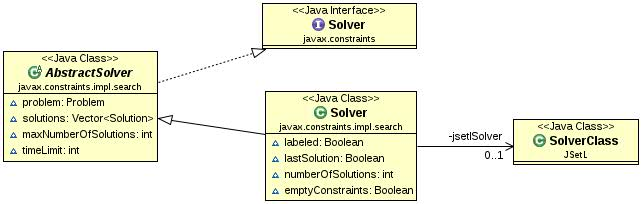
\includegraphics[scale=.5]{img/Solver.JPG}
\caption{Class Diagram di \texttt{Solver}.}
\end{figure}

\subsubsection{Attributi}
La specifica JSR-331, contrariamente a
quanto visto per le variabili ed i vincoli, non prevede che uno specifico
CP solver implementi una classe apposita per un entità solver. Questo 
approccio è ragionevole e non è quindi prevista una struttura come 
\files{CommonBase} in cui sia possibile impostare una implementazione concreta
mediante \files{setImpl}.

Tuttavia JSetL fornisce una classe (\files{SolverClass}) che implementa 
alcune delle proprietà richieste dall'interfaccia \files{Solver}, quindi  viene
utilizzato come attributo \files{private} un'istanza di \files{SolverClass}.
Si elencano di seguito gli attributi aggiunti rispetto alla classe di base:

\begin{lstlisting}[language = Java,
                   caption = {attributi di Solver.}]
	private SolverClass jsetlSolver;
	Boolean lastSolution = false;
	int numberOfSolutions;

	protected JSetL.Constraint[] jsetlConstraints;
	Boolean emptyConstraints = false;
\end{lstlisting}
Come già detto, il primo attributo rappresenta il solver concreto di JSetL.
Segue un attributo booleano: \files{lastSolution} che
indica se nel processo di ricerca si è arrivati all'ultima soluzione valida
per il corrente solver \files{jsetlSolver}. L'attributo
intero rappresentante il corrente numero di soluzioni trovate.

I due attributi separati sono d'ausilio per il passaggio dei vincoli dal
problema a cui il solver è legato al solver JSetL.

\subsubsection{Costruttori}
Vi è un solo costruttore richiesto, che prende come parametro il problema su
cui si costruisce il solver.

\begin{lstlisting}[language = Java,
                   caption = {costruttore di base.}]
public Solver(Problem problem) {
        super(problem);
        jsetlSolver = new SolverClass();
        numberOfSolutions = 0;
        getProblemConstraints();
        setProblemConstraints();
}
\end{lstlisting}
Qui viene chiamato il costruttore della classe astratta di base con il solito
costrutto \files{super(problem)}, quindi viene istanziato l'attributo
\files{jsetlSolver} mediante il suo costruttore. Il numero di soluzioni è
impostato a $0$. Una volta inizializzati i membri propri della classe, mediante
i metodi privati \texttt{getProblemConstraints} e \texttt{setProblemConstraints}
vengono caricati i vincoli presenti nel problema (al momento dell'istanziazione
del solver) e quindi salvati nello \emph{store} JSetL.

\begin{lstlisting}[language = Java,
                   caption = {metodi privati per caricare i vincoli.}]
private void setProblemConstraints() {
        if (emptyConstraints) 
                return;
        for (JSetL.Constraint c : jsetlConstraints)
                jsetlSolver.add(c);
}

private void getProblemConstraints() {
        jsetlConstraints = ((Problem) getProblem()).getJSetLConstraints();
        if (jsetlConstraints == null)
                emptyConstraints  = true;
        else emptyConstraints = false;
}
\end{lstlisting}


\subsubsection{Metodo \texttt{newSearchStrategy}}
\files{newSearchStrategy} è un metodo che consente all'utente di creare una 
nuova strategia di ricerca
per il solver specifico, \files{Solver} in questo caso funziona praticamente 
come una factory.
\begin{lstlisting}[language = Java,
                   caption = {\files{newSearchStrategy}.}]
	public SearchStrategy newSearchStrategy() {
		return new SearchStrategy(this);
	}
\end{lstlisting}
Questo metodo restituisce semplicemente la chiamata ad un costruttore della
classe \files{SearchStrategy}.

\subsubsection{Risoluzione del problema}
Questa parte sella sezione è dedicata alla ricerca delle soluzioni, verranno qui
definiti i metodi \files{findSolution},  \files{findOptimalSolution} e 
\files{findAllSolutions}.

\subsubsection{Metodo \texttt{findSolution}}
Il metodo \files{findSolution} di cui viene richiesta l'implementazione nelle
specifiche è quello con parametro (\files{ProblemState}). Tale parametro
definisce se, dopo la ricerca, lo stato del problema vada ristabilito o meno.

\begin{lstlisting}[language = Java,
                   caption = {\files{findSolution}.}]  
public Solution findSolution(ProblemState restoreOrNot) { 
  applyHeuristic();
  Solution solution = null;
  if(restoreOrNot == ProblemState.RESTORE) {
      .
      .
      .
  } else if(restoreOrNot == ProblemState.DO_NOT_RESTORE) { 
      try { 
        jsetlSolver.solve(); 
        solution = new Solution(this,  
                      numberOfSolutions++); 
      } catch (Failure e) {
          solution = null; 
          e.printStackTrace(); 
        } 
  } 
  return solution;  
}
\end{lstlisting}
Il metodo applica le euristiche sulle variabili del problema con
\files{applyHeuristic}, che verrà discusso in seguito, quindi procede con la
ricerca della soluzione.

A questo punto la computazione ha un punto di scelta, ovvero se lo stato del 
problema va ristabilito al termine della ricerca o meno. 

Il caso \texttt{DO\_NOT\_RESTORE}, più semplice del primo, applica
semplicemente il metodo \files{solve} al solver JSetL, che se troverà una 
soluzione verrà salvata nella variabile \texttt{solution}, altrimenti 
sarà lanciata un'eccezione e catturata subito dopo, impostando a \texttt{null}
la variabile stessa. Il costruttore di 
\files{Solution}, come vedremo nella sezione \ref{jsetlSolution},
salverà ogni variabile del problema internamente.

\begin{lstlisting}[language = Java,
                   caption = {\files{findSolution} il caso \texttt{RESTORE}.}] 
    if(restoreOrNot == ProblemState.RESTORE) {
            if(jsetlSolver.check()) {
                    lastSolution = false;
                    try {
                         solution = new Solution(this, 
                                    numberOfSolutions++);
                    } catch (Failure e) {
                            e.printStackTrace();
                            return null;
                    }
            }
            else return null;
    }
\end{lstlisting}
Il parametro \texttt{RESTORE} è utilizzato principalmente dal metodo
\texttt{hasNext} della classe \texttt{SolutionIterator}. Concettualmente
il suo significato può essere espresso come il ripristino dello stato del 
problema fino all'ultimo punto di scelta, per poter generare quindi la soluzione
successiva. Per implementare questo concetto si è optato per utilizzare la
funzione \texttt{check} del solver JSetL che consente di generare una soluzione
senza svuotare il \texttt{constraint store}.

\subsubsection{Metodo \texttt{findOptimalSolution}}
Come suggerisce il nome, questo metodo ricerca una soluzione ottimale per il
problema. Per fare ciò l'algoritmo dovrebbe esplorare l'intero spazio delle 
soluzioni e memorizzare quella più vicina all'obiettivo. In realtà si è adottato
un sistema per ridurre tale spazio, propagando vincoli sulla
variabile obiettivo, analogamente all'approccio adottato dall'implementazione
comune.
La descrizione del metodo verrà spezzata in più parti, poiché è piuttosto
lungo e composto da più istruzioni correlate.
\begin{lstlisting}[language = Java,
                   caption = {\files{findOptimalSolution}, inizializzazione.}]
public Solution findOptimalSolution(Objective objective, Var objectiveVar) {
	addObjective(objectiveVar);
	long startTime = System.currentTimeMillis();
	if (objectiveVar.getName().isEmpty())
		objectiveVar.setName("Objective"); 
	if (getProblem().getVar(objectiveVar.getName()) == null) {
		getProblem().add(objectiveVar);
	}
	javax.constraints.Var obj = objectiveVar;
	JSetL.Constraint c = new JSetL.Constraint();
	IntLVar target = (IntLVar) obj.getImpl();
	Boolean maximize = false;
	int bestValue = Integer.MAX_VALUE /2;
	if(objective.equals(Objective.MAXIMIZE)) {
		maximize = true;
		bestValue = - Integer.MAX_VALUE /2;
		c.and(target.gt(bestValue));
	} else 	c.and(target.lt(bestValue));
	Solution solution = null;  
\end{lstlisting}
Inizialmente il metodo deve occuparsi di definire l'obiettivo e la variabile
coinvolta. Se la variabile non ha un nome glie ne viene assegnato uno di
default, quindi si verifica che questa appartenga alle
variabili del problema, contrariamente viene aggiunta.

L'obiettivo della funzione può essere di minimizzare o massimizare il valore
della variabile data, a questo propostio viene creato un valore pessimo
\files{bestValue} che rappresenta il minimo o il massimo valore
rappresentabile a seconda del parametro \files{Objective} passato. Il nome
della variabile intera \files{bestValue}
potrebbe essere fuorviante, il valore infatti è quello pessimo per
l'obiettivo ma è considerato l'attuale valore migliore. Ad ogni passo 
se il nuovo valore \files{newValue} è migliore, \files{bestValue} verrà 
sostituito da questo.

A supporto di questo approccio viene utilizzato un vincolo JSetL \texttt{c}
relativo alla variabile obiettivo. Se tale variabile deve essere massimizzata
il valore \texttt{target} deve essere maggiore del miglior valore
attuale, viceversa dovrà essere minore.

\begin{lstlisting}[language = Java,
                   caption = {\files{findOptimalSolution}, il ciclo.}]
while(jsetlSolver.check(c)) {
	if(getMaxNumberOfSolutions() > 0 && 
			numberOfSolutions >= getMaxNumberOfSolutions())
		break;
	if(getTimeLimit() > 0) {
		if (System.currentTimeMillis() - startTime > getTimeLimit())
			break;				
	}
        numberOfSolutions++;
        try {
	    solution = new Solution(this, 
                    numberOfSolutions++);
	} catch (Failure e) {
		e.printStackTrace();
		return null;
	}
        .
        .
        .
\end{lstlisting}
Terminata l'inizializzazione si passa al ciclo per la ricerca vera e propria.
In questa parte del codice si evidenziano le condizioni di ingresso e di uscita 
dal ciclo.

Le istruzioni all'interno del \files{while} continuano fintanto che il vincolo
propagato \texttt{c} nel solver JSetL mediante la funzione \texttt{check}, 
è soddisfacibile. 
Internamente al ciclo si trova quindi una nuova soluzione e viene incrementato
di conseguenza il numero delle soluzioni.

Le possibili condizioni di uscita sono le seguenti:
\begin{enumerate}
\item \texttt{check} ritorna \texttt{false}, ovvero non esistono soluzioni
con l'attuale propagazione del vincolo \texttt{c};
\item è impostato un numero limite di soluzioni ed è stato raggiunto o superato;
\item è impostato un tempo limite ed è stato raggiunto o superato.
\end{enumerate}

\begin{lstlisting}[language = Java,
                   caption = {\files{findOptimalSolution}, verifica obiettivo.}
                  ]  
        int newValue;
        if(maximize) {
                newValue = solution.getMin(obj.getName());
                if(bestValue < newValue)
                        bestValue = newValue;
                c.and(target.gt(bestValue));
        }
        else {	
                newValue = solution.getMax(obj.getName());
                if(bestValue > newValue)
                        bestValue = newValue;
                c.and(target.lt(bestValue));
        }
\end{lstlisting}
Questa è la parte, interna al ciclo, che verifica l'obiettivo ed aggiorna 
l'eventuale soluzione ottima, inoltre aggiorna il vincolo che verrà poi
propagato nella successiva esecuzione della \texttt{check}. Ad ogni passaggio 
viene memorizzato il valore
della corrente soluzione nell'intero \files{newValue}, a seconda che 
l'obiettivo sia massimizzare o minimizzare, se il nuovo valore
è migliore di \files{bestValue}, questo viene sostituito.

Ogni volta viene aggiornato il vincolo relativo alla variabile obiettivo: se
occorre massimizzare il vincolo sarà del tipo $\files{target} > 
\files{newValue}$,
altrimenti del tipo  $\files{target} < \files{newValue}$.
\begin{lstlisting}[language = Java,
                   caption = {\files{findOptimalSolution}, termine.}
                  ]
if (solution != null)
   log("Optimal solution is found. Objective: " +solution.getValue(objectiveVar.getName()));
   return solution;
}
\end{lstlisting}

\subsubsection{Metodo \texttt{findAllSolutions}}
L'ultimo metodo implementato per la ricerca delle soluzioni è inerente alla
ricerca di tutte le possibili soluzioni del problema. Come visto per
\files{findSolution} questo metodo applica prima un'euristica per le
variabili ed i valori, poi si occupa della ricerca.

\begin{lstlisting}[language = Java,
                   caption = {\files{findAllSolutions}, inizializzazione.}
                  ]
public Solution[] findAllSolutions() {
  ArrayList<Solution> array = new ArrayList<Solution>();
  applyHeuristic();
  long startTime = System.currentTimeMillis();
  if(jsetlSolver.check() && (this.getMaxNumberOfSolutions() > 0 || this.getMaxNumberOfSolutions() == -1)) {
    
          .
          .  // Ricerca di tutte le soluzioni.
          .
    
  }
  else return null;
  .
  .
  .
\end{lstlisting}
Inizialmente viene creato un nuovo \files{ArrayList} che conterrà le soluzioni
trovate nel processo di risoluzione. Vengono applicate le euristiche su ogni
variabile del problema e quindi viene inizializzato il timer per il controllo
tempo limite.

A questo punto il metodo è pronto ad iniziare la ricerca, mediante l'istruzione 
\files{if} viene controllato che il problema sia soddisfacibile 
(\files{check}) e il numero
di soluzioni sia coerente con la richiesta. All'interno del ciclo 
è definita la ricerca delle soluzioni.

\begin{lstlisting}[language = Java,
                   caption = {\files{findAllSolutions}, ricerca.}
                  ]
	do { 
	    if (getTimeLimit() > 0) {
		if (System.currentTimeMillis() - startTime > 
		getTimeLimit())
                   break;				
	    }
	    Solution solution;
	    try {
		solution = new Solution(this, 
		numberOfSolutions++);
	    } catch (Failure e) {
	        solution = null;
	        e.printStackTrace();
	    }
	    array.add(solution);
	} while(jsetlSolver.nextSolution() && 
		((this.getMaxNumberOfSolutions() > 
		numberOfSolutions) ||
		this.getMaxNumberOfSolutions() == -1));
\end{lstlisting}
Questa parte di codice, interna al ciclo, genera una soluzione mediante il
solito costruttore quindi l'aggiunge al vettore delle soluzioni. Si entra nel 
ciclo solo se una soluzione è ammissibile.

Le condizioni di uscita del ciclo sono le seguenti:
\begin{enumerate}
\item non esiste una nuova soluzione e quindi l'ultima valida è effettivamente
quella aggiunta nell'array;
\item si è superato il numero di soluzioni massime e quindi l'ultima soluzione
trovata era quella con numero massimo;
\item si è raggiunto o superato il tempo limite.
\end{enumerate}

A questo punto, poiché il metodo richiede che venga restituito un array di 
soluzioni (e non un \files{ArrayList}), questo viene creato e restituito:
\begin{lstlisting}[language = Java,
                   caption = {\files{findAllSolutions}, calcolo del risultato.}
                  ]
  Solution[] result = new Solution[array.size()];
  for (int i = 0; i < result.length; i++) {
    result[i] = array.get(i);
  }
  return result;
}
\end{lstlisting}

\subsubsection{Metodi ausiliari}
Questa parte della sezione è dedicata alle funzioni ausiliarie all'interno
della classe, tra i metodi più rilevanti si evidenziano:
\begin{lstlisting}[language = Java, frame = single]
private void applyHeuristic();
public void addJSetLConstraint(JSetL.Constraint c);
\end{lstlisting}
Ogni metodo sopra elencato è importante perché influenza il solver aggiungendo
vincoli al problema.

\subsubsection{Metodo \texttt{applyHeuristic}}
Questo metodo aggiunge al solver (\files{jsetlSolver}) i vincoli che hanno a che
fare con le euristiche di scelta delle variabili e dei valori che si vogliono
assegnare.
\begin{lstlisting}[language = Java,
                   caption = {\files{applyHeuristic}.}
                  ]
private void applyHeuristic() {
  Vector<javax.constraints.SearchStrategy> strategies = 
      getSearchStrategies();
  if (strategies.isEmpty()) {
    SearchStrategy strategy = (SearchStrategy) getSearchStrategy();
    strategy.label();
    strategy.labelSets();
  }
  else {
       for (int i = 0; i < strategies.size(); i++) {
         SearchStrategy strategy = strategies.elementAt(i);
         ((SearchStrategy) strategy).label();
         ((SearchStrategy) strategy).labelSets();
       }
   }
}
\end{lstlisting}
Il metodo  carica semplicemente le strategie di ricerca in un 
\files{Vector}. Se nessuna strategia è stata precedentemente definita ne
viene creata una di default mediante il metodo \files{getSearchStrategy}, quindi
vengono chiamati i metodi di labeling della classe \files{SearchStrategy}.
Se sono state caricate più di una strategia, per ognuna di esse viene 
effettuato il labeling.

\subsubsection{Metodo \texttt{addJSetLConstraint}}
Il metodo in questione è utilizzato per aggiungere un vincolo JSetL direttamente
al solver \files{jsetlSolver}.
\begin{lstlisting}[language = Java,
                   caption = {\files{addJSetLConstraint}.}
                  ]
public void addJSetLConstraint(JSetL.Constraint c) {
	jsetlSolver.add(c);
}
\end{lstlisting}



\section{Interfaccia \texttt{SearchStrategy}}
La specifica JSR-331 utilizza il concetto di Search Strategy per permettere
ad un utente di scegliere tra differenti algoritmi di ricerca forniti
dalle differenti implementazioni. Le strategie di ricerca sono utilizzate
dai metodi dei solver che si occupano di trovare una soluzione.

Una strategia di ricerca dovrebbe conoscere tutte le variabili di cui si dovrà
assegnare un valore e potrebbero essere necessari
selettori esterni per le variabili ed i valori.

Ogni solver dovrebbe fornire almeno una strategia di ricerca 
 di default da utilizzare nei costruttori del \files{Solver}.

\subsection{Lista d'esecuzione}
La lista d'esecuzione delle strategie di ricerca  consente agli utenti di 
mescolare le strategie per i diversi tipi di variabili e di controllare
l'ordine di assegnamento dei valori. Ad esempio, per la pianificazione e per
problemi di allocazione delle risorse, un utente può decidere prima di 
programmare tutte le attività e poi assegnare le risorse alle attività già 
programmate. Ma  può anche decidere di assegnare prima le risorse e solo 
allora di programmare le attività in base alla disponibilità delle risorse.

\`E stato quindi fornito un sistema per cui l'utente può specificare diverse
strategie per insiemi di variabili differenti. Il metodo della classe
\files{Solver}
\begin{center}
\lstinline[language = Java]$SearchStrategy newSearchStrategy();$
\end{center}
restituisce una nuova istanza per la strategia di default della particolare
implementazione JSR-331 in uso. L'utente può quindi specificare su questa
strategia delle euristiche per le variabili ed i valori e quindi aggiungere la
nuova strategia modificata alla lista d'esecuzione.

Di seguito si mostra un semplice esempio.
\begin{lstlisting}[language = Java,
                   caption = {due differenti strategie.}]
Solver solver = problem.getSolver();
SearchStrategy typeStrategy = solver.getSearchStrategy();
typeStrategy.setVars(types);
SearchStrategy countStrategy = solver.newSearchStrategy();
countStrategy.setVars(counts);
countStrategy.setVarSelectorType(VarSelectorType.MIN_DOMAIN);
solver.addSearchStrategy(countStrategy);
solution = solver.findSolution();
\end{lstlisting}
Sono presenti altri metodi utili per specificare strategie di ricerca senza
dover esplicitamente creare nuove istanze di \files{SearchStrategy}. Il
metodo \files{addSearchStrategy} ad esempio supporta differenti combinazioni di 
parametri \files{Var[]}, \files{VarSelector} e \files{ValueSelector}. Il codice 
di cui sopra può essere riscritto in un modo più conciso:
\begin{lstlisting}[language = Java,
                   frame = single]
Solver solver = problem.getSolver();
solver.getSearchStrategy().setVars(types);
solver.addSearchStrategy(counts, VarSelectorType.MIN_DOMAIN);
solution = solver.findSolution();
\end{lstlisting}

\subsection{Variable Selector}
JSR-331 specifica un insieme di selettori di variabili standard che possono
essere usati dall'utente per personalizzare la strategia. Queste
euristiche sono definite dall'interfaccia standard \files{VariableSelector}
utilizzando il seguente tipo enumerativo:
\begin{lstlisting}[language = Java,
                   frame = single]
static public enum VarSelectorType {
    INPUT_ORDER,
    MIN_VALUE,
    MAX_VALUE,
    MIN_DOMAIN,
    MIN_DOMAIN_MIN_VALUE,
    MIN_DOMAIN_RANDOM,
    RANDOM,
    MIN_DOMAIN_MAX_DEGREE,
    MIN_DOMAIN_OVER_DEGREE,
    MIN_DOMAIN_OVER_WEIGHTED_DEGREE,
    MAX_WEIGHTED_DEGREE,
    MAX_IMPACT,
    MAX_DEGREE,
    MAX_REGRET,
    CUSTOM
}
\end{lstlisting}
Non tutte queste euristiche devono essere fornite da ogni implementazione
concreta di JSR-331.

\subsection{Value Selector}
JSR-331 specifica un insieme di selettori di valori standard che possono
essere usati dall'utente per personalizzare la strategia. Queste
euristiche sono definite dall'interfaccia standard \files{ValueSelector}
utilizzando il seguente tipo enumerativo:
\begin{lstlisting}[language = Java,
                   frame = single]
static public enum ValueSelectorType {
    IN_DOMAIN,
    MIN,
    MAX,
    MIN_MAX_ALTERNATE,
    MIDDLE,
    MEDIAN,
    RANDOM,
    MIN_IMPACT,
    CUSTOM
}
\end{lstlisting}
Non tutte queste euristiche devono essere fornite da ogni implementazione
concreta di JSR-331.

\subsubsection{Euristiche in JSetL}
Prima di passare alla descrizione della classe \files{SearchStrategy} che
fornisce l'implementazione per le strategie di ricerca, occorre sottolineare
che l'approccio alle strategie di selezione delle variabili e dei valori è
differente da quello ipotizzato nella specifica.

La specifica presuppone che le variabili siano selezionate prima, per poi 
essere passate ad un risolutore che vi assegni un valore; infatti 
all'interno del \files{package} 
\files{javax.constraints.impl.search.selectors} fornito dalla specifica
sono definiti vari selettori predefiniti.

JSetL si basa su un sistema molto differente, sfruttando il solver ed 
aggiungendo vincoli di labeling, come già accennato nel capitolo \ref{jsetl} e 
come verrà sottolineato poco più avanti. Per questa ragione, le euristiche di
cui sopra sono state mappate su quelle definite in JSetL per il labeling.

\begin{notabene}
Di contro, questo approccio rende impossibile per l'utente definire una
propria strategia come invece la specifica descritta in \cite{specifiche} 
richiederebbe. 
\end{notabene}

\section{Classe \texttt{SearchStrategy}}\label{search}
La classe \files{SearchStrategy} implementa l'interfaccia standard 
 estendendo la classe \files{AbstractSearchStrategy} 
dell'implementazione comune.
\begin{lstlisting}[language = Java, frame = single]
public class SearchStrategy extends AbstractSearchStrategy {
\end{lstlisting}

Questo approccio permette di ereditare tutti i metodi astratti puri da 
implementare e, dove necessario, ridefinire i metodi non astratti.

\subsection{Classe \texttt{AbstractSearchStrategy}}
La classe astratta \files{AbstractSearchStrategy} estende la classe
\files{CommonBase} descritta nella sezione \ref{common}, poiché come
accennato precedentemente, la specifica si aspetta che ogni implementazione
concreta disponga di una classe che rappresenti la strategia.

JSetL non ha questa caratteristica, tuttavia si è deciso di utilizzare la
classe astratta poiché fornisce molti attributi e metodi utili.

\subsubsection{Attributi}
Gli attributi della classe \files{AbstractSearchStrategy} sono sei:
\begin{lstlisting}[language = Java, frame = single]
	Solver solver;
	protected Var[] vars;
	protected VarReal[] varReals;
//	protected VarSet[] varSets;
	protected VarSelector varSelector;
	protected ValueSelector valueSelector;
	SearchStrategyType type;
\end{lstlisting}
Il primo è il riferimento al solver a cui la strategia è legata.
Seguono quindi gli array delle variabili della strategia, come si può notare
l'array per le variabili insiemistiche è commentato. Durante lo studio della 
specifica si è cambiato approccio
per quanto riguarda le variabili insiemistiche.

Gli attributi \files{varSelector} e \files{valueSelector} specificano
le euristiche della strategia, mentre \files{type} ne definisce il tipo.

\begin{nota}
Per quanto riguarda l'implementazione concreta basata su JSetL due attributi 
verranno ignorati: \files{varReals} e \files{type}. Il primo perché attualmente 
non sono supportate variabili reali, mentre il secondo per la differenza di 
apporccio nell'applicazione delle euristiche, di fatto ogni strategia sarà di 
tipo \files{SearchStrategyType.DEFAULT}.
\end{nota}

\subsubsection{Metodi utili}
I metodi di utilità generica o che non hanno bisogno di un'implementazione
specifica come quella fornita da JSetL, vengono implementati 
direttamente all'interno della classe \texttt{AbstractSearchStrategy}.
Tra quelli più utilizzati si evidenziano:
\begin{itemize}
\item \lstinline[language=Java]$public Solver getSolver();$

Restituisce il solver associato alla strategia di ricerca.
\item \lstinline[language=Java]$public Var[] getVars();$

Restituisce un array di variabili associate alla strategia d'invocazione.
\item \lstinline[language=Java]$public void setVars(Var[] vars);$

Associa un array di variabili alla strategia d'invocazione.
\item \lstinline[language=Java]$public ValueSelector getValueSelector();$

Restituisce l'euristica di selezione del valore da assegnare alle variabili.
\item \lstinline[language=Java]$public VarSelector getVarSelector();$

Restituisce l'euristica di selezione delle variabili.
\item \lstinline[language=Java]$public void setValueSelector(ValueSelector valueSelector);$

Imposta l'euristica di selezione del valore da assegnare alle variabili.
\item \lstinline[language=Java]$public void setVarSelector(VarSelector varSelector);$

Imposta l'euristica di selezione delle variabili.
\end{itemize}

Altri metodi, come ad esempio \files{setVars} sulle variabili insiemistiche,
sono stati omessi poiché non utilizzati dall'implementazione basata su JSetL
oppure perché sovrascritti dalla stessa, e verranno quindi definiti nella
prossima sezione.

\subsection{Implementazione}
Come già sottolineato nel capitolo, JSetL ha un approccio diverso da quello
previsto dalla specifica, l'implementazione quindi non si avvale appieno
delle funzionalità della classe \files{AbstractSearchStrategy} e della
\files{CommonBase}. Inoltre, utilizzando un approccio diverso anche per
l'implementazione delle variabili insiemistiche si è dovuto specializzare
ulteriormente la classe con attributi e metodi.

\begin{figure}[!ht]\label{searchstrategyUML}
\centering
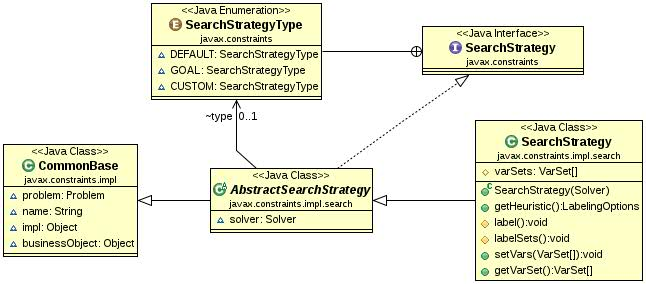
\includegraphics[scale=.5]{img/SearchStrategy.JPG}
\caption{Class Diagram di \texttt{SearchStrategy}.}
\end{figure}

\subsubsection{Attributi}
Poiché nel problema (nella classe \files{Problem}) è stato aggiunto 
un array di variabili insiemistiche legate al problema, anche nella classe 
\files{SearchStrategy}
è stato aggiunto tale array.
\begin{lstlisting}[language = Java, frame = single]
    protected VarSet[] varSets;
\end{lstlisting}
L'attributo \files{varSets} rappresenta le variabili insiemistiche associate 
alla strategia.

\subsubsection{Costruttori}
Vi è un solo costruttore di classe, che prende come unico argomento il
solver a cui è associato:
\begin{lstlisting}[language = Java, frame = single]
public SearchStrategy(Solver solver) {
	super(solver);
	varSets = ((Problem) getProblem()).getSetVars();
}
\end{lstlisting}
Questo chiama il costruttore della classe base, quindi inizializza i due
array mediante la funzione \files{getProblem} che restituisce il problema a 
cui la strategia è associata e quindi da questo ottiene le variabili con
il relativo metodo \files{getSetVars}.

\subsubsection{Euristiche}
In questa parte della sezione verranno specificati i metodi che codificano
ed applicano le euristiche di scelta per assegnare valori alle variabili
e per scegliere l'ordine di assegnamento delle stesse.

\subsubsection{Metodo \texttt{getHeuristic}}
Questa funzione è una vera e propria mappa per le euristiche, ovvero associa
ogni \files{VarSelector} o \files{ValueSelector} della specifica ad
un'euristica di JSetL. La funzione è divisa in due parti, la prima si occupa
delle variabili, la seconda dei valori.
\begin{lstlisting}[language = Java,
                   caption = {\files{getHeuristic}, le variabili.}]
public LabelingOptions getHeuristic() {
	LabelingOptions lop = new LabelingOptions();
	VarSelector varSelector = getVarSelector();
	if (varSelector != null) {
		VarSelectorType varType = varSelector.getType();
		switch(varType) {
		case INPUT_ORDER: 
			lop.var = VarHeuristic.LEFT_MOST;
			break;
		case MIN_VALUE:
			lop.var = VarHeuristic.MIN;
			break;
		case MAX_VALUE:
			lop.var = VarHeuristic.MAX;
			break;
		case RANDOM:
			lop.var = VarHeuristic.RANDOM;
			break;
		case MIN_DOMAIN:
			lop.var = VarHeuristic.FIRST_FAIL;
			break;
		default:
			lop.var = VarHeuristic.LEFT_MOST;
			break;
		}
	}
	else lop.var = VarHeuristic.LEFT_MOST;
\end{lstlisting}
Innazitutto viene inizializzata un'istanza della classe
\files{LabelingOptions}, questa è una classe di supporto JSetL utile per 
definire vincoli di labeling sulle variabili, ovvero le euristiche.

Quindi, mediante il metodo della classe base \files{getVarSelector}, viene
memorizzato il selettore per le variabili. Con lo \files{switch} infine, a 
seconda del caso viene impostato il valore di \files{lop.var} opportuno.
Se nessuno dei casi combacia con quelli identificati viene imposto di default
un'euristica di tipo leftmost, come richiesto dalla specifica.
\begin{lstlisting}[language = Java,
                   caption = {\files{getHeuristic}, i valori.}]
    ValueSelector valueSelector = getValueSelector();
    if (valueSelector != null) {
	ValueSelectorType valueType = valueSelector.getType();
        switch(valueType) {
	case MIN:
		lop.val = ValHeuristic.GLB;
		break;
	case MAX:
		lop.val = ValHeuristic.LUB;
		break;
	case MIDDLE:
		lop.val = ValHeuristic.MID_MOST;
		break;
	case MEDIAN:
		lop.val = ValHeuristic.MEDIAN;
		break;
	case RANDOM:
		lop.val = ValHeuristic.EQUI_RANDOM;
		break;
	default:
		lop.val = ValHeuristic.GLB;
		break;
	}
	return lop;
\end{lstlisting}
Nella parte finale dell'algoritmo si compiono gli stessi passaggi, ma per
la scelta dei valori. Quindi viene restituito il \files{LabelingOptions}
ottenuto.

\subsubsection{Metodo \texttt{label}}
Il metodo \files{label} è il primo metodo implementato e descritto che si
occupa di applicare un'euristica. Questo opera sulle variabili intere della 
strategia.
\begin{lstlisting}[language = Java,
                   caption = {\files{label()}.}]
protected void label() {
	if (vars == null || vars.length == 0)
		return;
	SolverClass sc = ((Solver) getSolver()).getSolverClass();
	IntLVar[] vec = new IntLVar[vars.length];
	for (int i = 0; i < vars.length; i++) {
		vec[i] = (IntLVar) vars[i].getImpl();
	}
	sc.add(IntLVar.label(vec, getHeuristic()));
}
\end{lstlisting}
Dopo aver controllato che il vettore delle variabili intere non sia nullo
(contrariamente il metodo viene interrotto senza errori) viene memorizzato
un riferimento al solver JSetL e viene inizializzato un vettore di
\files{IntLVar} con le implementazioni concrete delle variabili intere
della strategia.

A questo punto viene caricata la strategia mendiante il metodo
\files{getHeuristic} vista sopra, ed aggiunto al solver JSetL un vincolo
speciale di labeling creato mediante la funzione
\files{label(IntLVar[], LabelingOptions)} definita in \cite{tesiAmadini} e di 
cui si
è accennato nel capito \ref{jsetl}.

\subsubsection{Metdo \texttt{labelSets}}
\files{labelSets} si comporta come il metodo per le variabili intere, cambiano
solo i tipi, tecnica e metodi sono i medesimi, si da la definizione per 
completezza.
\begin{lstlisting}[language = Java,
                   caption = {\files{labelSets()}.}]
protected void labelSets() {
	if (varSets == null || varSets.length == 0)
		return;
	SolverClass sc = ((Solver) getSolver()).getSolverClass();
	SetLVar[] vec = new SetLVar[varSets.length];
	for (int k = 0; k < vars.length; k++) {
		vec[k] = (SetLVar) varSets[k].getImpl();
	}
	sc.add(SetLVar.label(vec, getHeuristic()));
}
\end{lstlisting}

\section{Interfaccia \texttt{Solution}}
L'interfaccia standard \files{Solution} specifica le soluzioni che possono
essere generate dai metodi della classe \files{Solver} e dagli iteratori.
Questa interfaccia è completamente implementata nella common implementation
definita dalla classe \files{BasicSolution},
ogni implementazione concreta può estenderla mediante la sottoclasse
\files{Solution}.

Un'istanza della soluzione contiene le copie di tutte le variabili
legate al problema che sono state usate da una strategia di ricerca che ha
creato tale soluzione.

\subsubsection{Metodi}
I metodi e le funzioni definiti nell'interfaccia sono i seguenti:
\begin{itemize}
\item[-]\lstinline[language = Java]$public Var[] getVars();$

Restituisce le variabili della soluzione legate al problema.
\item[-]\lstinline[language = Java]$public Var getVar(String name);$

Restituisce la variabile con il nome dato dalla stringa \files{name}. 
Lancia un'eccezione se la variabile non esiste.
\item[-]\lstinline[language = Java]$public int getValue(String name);$

Restituisce il valore della variabile con il nome dato dalla stringa 
\files{name}. 
Lancia un'eccezione se la variabile non esiste.
\item[-]\lstinline[language = Java]$public boolean isBound();$

Restituisce \files{true} se ogni variabile della soluzione è bound (ovvero
il suo dominio è un singolo valore), \files{false} altrimenti.
\item[-]\lstinline[language = Java]$public boolean isBound(String name);$

Restituisce \files{true} se la variabile con il nome dato  è ``bound'',
\files{false} altrimenti.
\item[-]\lstinline[language = Java]$public int getSolutionNumber();$

Restituisce il numero associato alla soluzione.
\item[-]\lstinline[language = Java]$public void setSolutionNumber(int number);$

Assegna un valore intero al numero associato alla soluzione.
\item[-]\lstinline[language = Java]$public void log();$

Questo metodo stampa la soluzione, è una variante della medesima definita
nell'interfaccia \files{Problem}.
\item[-]\lstinline[language = Java]$public Solver getSolver();$

Restituisce il solver associato alla soluzione.
\end{itemize}

\section{Classe \texttt{Solution}}\label{jsetlSolution}
La classe \files{Solution} implementa l'interfaccia standard
\files{Solution} estendendo la classe \files{BasicSoltion} dell'implementazione
comune.
\begin{lstlisting}[language = Java,
                   frame = single]
public class Solution extends BasicSolution {
\end{lstlisting}
Questo approccio permette di ereditare tutti i metodi della classe base, che
non è astratta, ma una vera e propria implementazione di base
della soluzione. Verrà quindi brevemente descritta.

\subsection{Classe \texttt{BasicSolution}}
\files{BasicSolution} rappresenta l'implementazione di base della soluzione
di un problema, viene fornita nella specifica dal file 
\files{BasicSolution.java} contenuto nel package 
\files{javax.constraints.impl.search}. \`E una classe base, non
estende quindi nessun'altra classe
\begin{lstlisting}[language = Java,
                   frame = single]
public class BasicSolution implements Solution {
\end{lstlisting}

Questa classe implementa totalmente quanto specificato nell'interfaccia, 
pertanto non vi sarebbe il bisogno di specializzarla. Tuttavia poiché nella
implementazione basata su JSetL sono stati introdotti alcuni aspetti che
si discostano dalle specifiche individuate dallo standard, si è dovuto trattare
in modo specializzato quest'ultimi.

\subsubsection{Attributi}
Gli attributi della classe base sono i seguenti:
\begin{lstlisting}[language = Java,
                   frame = single]
	Solver 	        solver;
	int 		solutionNumber;
	ResultInt[] 	intResults;
	ResultReal[] 	realResults;
	ResultSet[] 	setResults;
\end{lstlisting}
\files{solver} rappresenta, come di consueto, il solver da cui la soluzione
è stata generata. L'intero \files{solutionNumber} ne rappresenta il numero
progressivo.

Gli utlimi tre attributi meritano un discorso più dettagliato, questi infatti 
sono degli array di un tipo definito nello stesso file della classe
\files{BasicSolution} e di fatto rappresentano internamente il risultato.

\subsubsection{Classe \texttt{ResultInt}}
\files{ResultInt} rappresenta una delle variabili intere risolta dal solver.
\begin{lstlisting}[language = Java,
                   frame = single]
class ResultInt {
	String varName;
	int value;
	inte min;
	int max;
	boolean bound;
}
\end{lstlisting}
Ha alcuni attributi che ne rappresentano il nome, il valore attuale (se 
unico), il valore minimo e quello massimo, quindi un booleano che indica 
se la variabile risolta è bound, ovvero ha un unico valore possibile. 
Viene fornita anche una funzione \files{toString}.

\subsubsection{Classe \texttt{ResultReal}}
Questa classe è praticamente identica a quella definita per le variabili
intere (cambiano ovviamente i tipi) e, poiché JSetL non supporta i vincoli
sui reali, verrà omessa la descrizione.

\subsubsection{Classe \texttt{ResultSet}}
Anche in questo caso verrà omessa la descrizione della classe, poiché
l'approccio adottato dallo standard è molto differente dall'implementazione
concreta che JSetL fornisce per gli insiemi. Tuttavia a differenza della
struttura sui reali, questa verrà ridefinita nel file della classe
\files{Solution}.

\subsubsection{Metodi}
Si evidenziano alcuni metodi non presenti tra quelli già menzionati 
nelle interfacce che manipolano le sopracitate classi di risultati:
\begin{itemize}
\item[-]\lstinline[language = Java]$private int getIndexOfInt(String name);$

Restituisce l'indice della variabile risolta di nome \files{name}. In caso
la variabile non esista lancia un'eccezione.
\item[-]\lstinline[language = Java]$ResultInt createResult(Var var);$

Questa importante funzione, presa una variabile intera (risolta dal solver),
genera e restituisce un istanza della classe \files{ResultInt}.
\end{itemize}

Al momento della realizzazione dell'implementazione concreta 
lo standard non fornisce il supporto alle variabili reali ed 
insiemistiche. Ovvero nel costruttore di \files{BasicSolution} non è ancora 
implementato l'algoritmo
per generare variabili risolte di tipo \files{ResultReal} e \files{ResultSet}.
Analogamente non è stata introdotta la funzione \files{createResult} per
le suddette variabili. Come si vedrà nella prossima sezione questi meccanismi
per le variabili insiemistiche sono state aggiunte nella specializzazione
\files{Solution}.

\begin{figure}[!ht]\label{solutionUML}
\centering
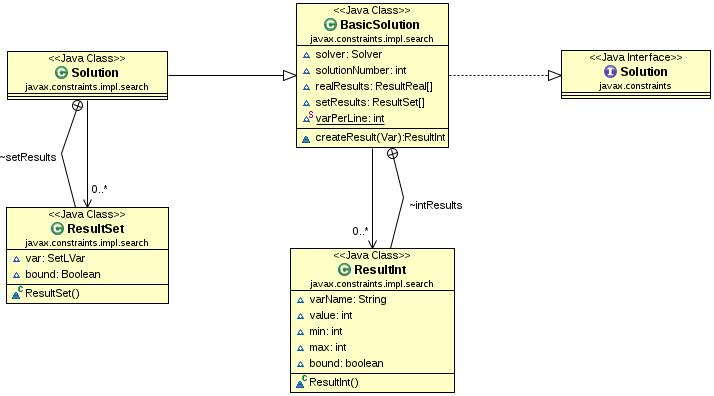
\includegraphics[scale=.5]{img/Solution.JPG}
\caption{Class Diagram di \texttt{Solution}.}
\end{figure}

\subsection{Implementazione}
La parte implementativa dell'interfaccia \files{Solution} verte esclusivamente
sul supporto delle variabili insiemistiche. Per raggiungere tale obiettivo si
è ridefinita la classe \files{ResultSet}, si è aggiunto un attributo come nella
classe base, si è definita la funzione \files{createResult} per variabili
insimistiche e si è specializzato il costruttore.


\subsubsection{Attributi}
L'unico attributo di classe è \files{setResults}, un array di tipo 
\files{ResultSet}. Questo attributo si è dovuto aggiungere causa l'impossibilità
di accedere alla controparte della classe base. Come questa, conterrà
un array di variabili risolte di tipo insiemistico.

\subsubsection{Classe \texttt{ResultSet}}
Come anticipato nella sezione precedente, la classe ausiliaria \files{ResultSet}
è stata ridefinita nel seguente modo:
\begin{lstlisting}[language = Java,
                   caption = {\files{ResultSet}.}]
class ResultSet {
	SetLVar var;
	Boolean bound;
	
	public String toString() {
		return var.toString();
	}
	
	public String getName() {
		return var.getName();
	}
}
\end{lstlisting}
Questa classe è stata creata sul modello di quelle implementate nel file 
dell'implementazione comune
\files{BasicSolution}, ma sfrutta la classe \files{SetLVar}.

\subsubsection{Metodo \texttt{createResult}}
Anche la funzione \files{createResult} è stata implementata seguendo l'approccio
di quella per variabili intere nella classe base.
\begin{lstlisting}[language = Java,
                 caption = {\files{createResult} per variabili insiemistiche.}]
private ResultSet createResult(VarSet var) {
        ResultSet result = new ResultSet();
        if(var.isBound())
                result.bound = true;
        else result.bound = false;
        result.var = (SetLVar) ((VarSet) var).getImpl();
        return result;
\end{lstlisting}
Data una variabile insiemistica \files{var}, questo metodo crea una nuova
istanza della classe \files{ResultSet} e quindi ne assegna i valori.
Se la data variabile è bound l'attributo \files{bound} della
nuova variabile risolta viene impostato a \files{true}, altrimenti a
\files{false}. Quindi nel campo \files{var} viene copiata 
l'implementazione concreta relativa alle variabili insimistiche.

\subsubsection{Costruttore}
La parte più delicata dell'implementazione è il costruttore. 
La descrizione di questo è stata
lasciata per ultima poiché sfrutta il tipo ed il metodo definiti sopra.
\begin{lstlisting}[language = Java,
                 caption = {\files{createResult} per variabili insiemistiche.}]
public Solution(Solver solver, int solutionNumber) throws Failure {
	super(solver, solutionNumber);
	Vector<javax.constraints.SearchStrategy> searchStrategies = 
            ((AbstractSolver)solver).getSearchStrategies();
	Vector<VarSet> strategyVars = new Vector<VarSet>();
	for (javax.constraints.SearchStrategy strategy : searchStrategies) {
		VarSet[] vars = ((SearchStrategy) strategy).getVarSet();
		if (vars == null)
			return;
		for (VarSet var : vars) {
			if (!strategyVars.contains(var))
				strategyVars.add(var);
		}
	}
	setResults = new ResultSet[strategyVars.size()];
	Iterator<VarSet> iter = strategyVars.iterator();
	int i = 0;
	while(iter.hasNext()) {
		VarSet var = iter.next();
		setResults[i++] = createResult(var);
	}	
}
\end{lstlisting}
Analogamente a quanto visto finora si è seguito l'approccio dell'implementazione
di base. Brevemente, il costruttore chiama quello della classe base, quindi
applica gli stessi costrutti per creare le variabili risolte ed inserirle 
nell'array dei risultati (specializzato).

Si evidenziano due fasi: nella prima vengono caricate tutte le strategie e 
per ogni strategia si salvano le variabili insimistiche coinvolte; nella
seconda fase viene creato l'array dei risultati che viene poi riempito
tramite la funzione \files{createResult}.


\section{Interfaccia \texttt{SolutionIterator}}
L'interfaccia standard \files{SolutionIterator} consente all'utente di trovare
e navigare tra diverse soluzioni ed eseguire differenti azioni specifiche
sulle soluzioni trovate.

L'utilizzo, come si intende nella specifica, è presentato in questo esempio:
\begin{lstlisting}[language = Java,frame = single]
SolutionIterator iter = solver.solutionIterator();
while(iter.hasNext()) {
  Solution solution = iter.next();
  ...
}
\end{lstlisting}

I metodi previsti dall'interfaccia sono solo due: \files{hasNext} che controlla
se c'è una nuova soluzione e \files{next} che genera la nuova soluzione.

\subsection{Classe \texttt{BasicSolutionIterator}}
L'implementazione comune fornisce una classe di base che implementa
l'interfaccia \files{SolutionIterator}. Questa non è stata presa in 
considerazione per
l'implementazione concreta JSetL e non verrà quindi descritta.

\section{Classe \texttt{SolutionIterator}}\label{solIter}
La classe \files{SolutionIterator} implementa l'interfaccia
\files{SolutionIterator} direttamente, senza appoggiarsi a classi di base.
\begin{lstlisting}[language = Java,frame = single]
public class SolutionIterator implements javax.constraints.SolutionIterator {
\end{lstlisting}


\subsubsection{Attributi}
Si definiscono i seguenti attributi:
\begin{lstlisting}[language = Java,frame = single]
	Solver solver;
	int solutionNumber;
	Boolean hasNext;
	Boolean checked = false;
        private boolean firstcall = true;
\end{lstlisting}
Come di consueto per le classi che rappresentano la soluzione, il primo 
attributo è il \files{solver} legato alla soluzione, quindi segue il numero
identificativo della stessa. \files{hasNext} è un valore booleano che
specifica se è presente una nuova soluzione, \files{checked} invece
è utilizzato per verificare che la funzione \files{hasNext} sia stata
invocata prima della funzione \files{next}. L'ultimo attributo verifica
che la funzione \texttt{hasNext} sia o meno invocata la prima volta.

\subsubsection{Costruttore}
L'unico costruttore richiesto è quello con parametro di tipo \files{Solver}:
\begin{lstlisting}[language = Java,
                   caption = {il costruttore di \files{SolutionIterator}.}]
public SolutionIterator(Solver s) {
	solver = (Solver) s;
	hasNext = true;
	solutionNumber = 0;
}
\end{lstlisting}
Questo imposta l'attributo \files{solver} con il solver che ha generato la
soluzione, imposta di default l'attributo \files{hasNext} a \files{true}
ed il numero di soluzione a $0$.

\subsubsection{Metodo \texttt{hasNext}}
Il metodo \files{hasNext} controlla che esista una soluzione successiva
all'interno dello stato del solver. Per fare ciò cerca una soluzione con il
metodo \files{findSolution} con parametro \files{ProblemState.RESTORE}, in
modo tale da permettere al solver di mantenere i punti di scelta ed iterare il
procedimento.
\begin{lstlisting}[language = Java,
                   caption = \files{hasNext}.]
public boolean hasNext() {
        checked = true;
        if (firstcall) {
                firstcall = false;
                Solution solution = solver.findSolution(ProblemState.RESTORE);
                if (solution == null) {
                        hasNext = false;
                        return false;
                }
                return true;
        }
        return solver.hasNext();
\end{lstlisting}
Inizialmente imposta \files{checked} al valore \files{true}, quindi se è 
la prima chiamata \texttt{firstcall} viene impostata a \texttt{true} quindi
cerca la soluzione.
Se la soluzione trovata non è nulla restituisce \files{true}, altrimenti
imposta l'attributo \files{hasNext} a \files{false} e restituisce
\files{false}.

Nel caso in cui la chiamata al metodo non è la prima, il risultato viene
demandato all'omonima funzione della classe \texttt{Solver} che semplicemente
sfrutta la funzione \texttt{nextSolution} del solver JSetL.


\begin{notabene}
\`E importante sottolineare che l'unico caso in cui viene usata la funzione
\files{findSolution} con il parametro \files{ProblemState.RESTORE}
all'interno dell'implementazione comune è nel relativo metodo \files{hasNext}
della classe \files{BasicSolutionIterator}.
Questo perché, secondo l'approccio utilizzato nella specifica JSR-331, 
\files{ProblemState} modella il controllo per il \emph{Backtracking}.

In JSetL il backtracking è insito nel solver e, per sfruttarlo, si utilizza la 
funzione
\files{nextSolution}, senza bisogno di un punto di
scelta. Per questo motivo, nella classe \files{Solver} il metodo
\files{findSolution} utilizza \files{nextSolution} nel
caso il parametro passato sia \files{RESTORE}.
\end{notabene}

\begin{figure}[!ht]\label{solutioniteratorUML}
\centering
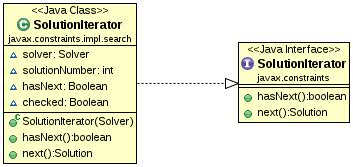
\includegraphics[scale=.75]{img/SolutionIterator.JPG}
\caption{Class Diagram di \texttt{SolutionIterator}.}
\end{figure}

\subsubsection{Metodo \texttt{next}}
Questo metodo crea la soluzione trovata dal metodo \files{hasNext} e la
restituisce. \`E quindi necessario che ogni volta che questo viene chiamato
sia stato precedentemente invocato \files{hasNext}. A questo proposito
viene sfruttato l'attributo \files{checked}: inizialmente il medoto controlla
che questo sia \files{true} (ovvero \files{hasNext} è stato utilizzato),
quindi prima dell'uscita lo reimposta a \files{false}, in modo tale che
\files{hasNext} debba essere richiamato nuovamente in seguito.

\begin{lstlisting}[language = Java,
                   caption = \files{next}.]
public Solution next() {
	if (!checked)
		throw new RuntimeException("Cannot use SolutionIterator.next() " + "before checking the hasNext() returned true");
	Solution solution;
	try {
		solution = new Solution(solver, solutionNumber);
		solution.setSolutionNumber(solutionNumber);
		solutionNumber++;
	} catch (Failure e) {
		e.printStackTrace();
		hasNext = false;
		return null;
	}
	checked = false;
	return solution;
}
\end{lstlisting}
All'interno del metodo viene creata la soluzione mediante il costruttore
fornito dalla classe \files{Solution} che automaticamente genera
le variabili risolte. Viene quindi aggiornato il numero di soluzione.



\hyphenation{
Jacob
Feldman
}

\chapter{Conclusioni e lavori futuri}\label{conclusioni}

Il lavoro di tesi descritto verte sull'implementazione delle
specifiche individuate dal JSR-331 mediante il pacchetto JSetL.
Il modello di sviluppo utilizzato per il progetto può essere catalogato come
\emph{in cascata} in cui si sono eseguite più iterazioni delle seguenti fasi:
\begin{enumerate}[i]
\item \label{i}Studio del documento di specifica \cite{specifiche}.
\item \label{ii}Valutazione delle funzionalità offerte da JSetL.
\item \label{iii}Codifica.
\item \label{iv}Test e validazione.
\end{enumerate}
Prima di passare alla descrizione delle fasi indicate occorre sottolineare
che tutto il lavoro non si sarebbe potuto svolgere senza l'appoggio del
Dr. Jacob Feldman, il quale, oltre ad un contatto diretto e grande 
disponibilità, ha fornito l'accesso al repository del  progetto e uno spazio
dedicato all'implementazione JSetL. Dal repository, mediante \emph{SVN}, si
è potuto scaricare tutto il materiale necessario per iniziare l'implementazione,
inoltre il repository
è stato uno strumento fondamentale per mantenere il progetto aggiornato.

Per quanto riguarda il punto \ref{i} si è trattato di analizzare il documento di
specifica fornito. Sono stati molto utili, al fine di comprendere meglio i 
requisiti dei vari metodi e delle classi, anche gli esempi presenti nel TCK
(vedi cap. \ref{capJSR}).

La valutazione di JSetL (punto \ref{ii}) è stata facilitata dai numerevoli 
documenti
(articoli, tesi, \ldots) presenti al Dipartimento di Matematica, nonché dal
contatto diretto con persone che hanno lavorato attivamente al 
progetto, su tutti il prof. Gianfranco Rossi, promotore del progetto e 
sempre disponibile.

La fase di codifica ha portato alla realizzazione vera e propria delle classi
descritte nei capitoli precedenti. Indubbiamente lo sforzo maggiore è
stato quello di mappare i requisiti di input e di output richiesti sulle 
funzionalità di JSetL in modo corretto ed efficace. In questa fase, oltre
alla codifica delle classi, si sono realizzati anche i test di unità, ovvero
delle prove d'esecuzione (white box) scritte appositamente per verifiche 
interne.

L'ultima fase riguarda il TCK che di fatto rappresenta l'unico test di
conformità alle specifiche. Come accennato nel capitolo \ref{capJSR} il TCK è
fornito direttamente dalle specifiche JSR-331 ed un'implementazione, per
essere conforme allo standard, deve permettere a questi test di terminare con 
successo. Nelle varie iterazioni del processo di sviluppo si è utilizzato
questo pacchetto per validare le unità introdotte e per poter quindi
passare alla realizzazione del modulo successivo o rivalutare quello non
soddisfacente. Oltre al TCK si è sviluppato un ulteriore pacchetto di test
per verificare l'implementazione prodotta allo scopo di coprire il più
possibile il codice. Tale attività è stata svolta nelle ultime
iterazioni del processo, nel momento in cui il TCK ha dato un buon numero di
successi.

Il lavoro svolto, essendo completamente modulare e documentato oltre che dal
presente testo anche mediante una ricca documetazione JavaDoc, risulta
facilmente estendibile e modificabile. 

\section{Sviluppi futuri}
La specifica JSR-331, al momento dell'inizio del progetto, era in fase di 
valutazione da parte del Java Community Process. Durante la stesura del
presente testo la specifica è stata accettata ed è passata da uno stato di
richiesta allo stato di release finale. Tuttavia, come annunciato nel
blog (\cite{blog}) del Dr. Jacob Feldman, questo rappresenta una milestone del
progetto di standardizzazione e JSR-331 sarà sviluppato ulteriormente. Per tale
motivo uno dei lavori futuri sarà quello di mantenere allineata 
l'implementazione
basata su JSetL con le specifiche. Si può notare che
l'implementazione fornita è solo una delle possibili, sarebbe
possibile analizzare più in dettaglio il pacchetto JSetL e le sue funzionalità
al fine di migliorare l'implementazione attuale. 
\`E anche doveroso
sottolineare che durante lo sviluppo del progetto sono emerse funzionalità
richieste che si è dovuto aggiungere e quindi anche il JSR-331 
rappresenta uno spunto per migliorare JSetL stesso.
Inoltre essendo JSetL un progetto didattico, è soggetto naturalmente a frequenti
cambiamenti e sarà quindi importante studiare la possibilità di utilizzare
nuove funzionalità.
Infine si evidenzia la possibilità di produrre un report, in fase di stesura,
nella forma di un Rapporto Tecnico del Dipartimento di Matematica, che possa
guidare nell'implementazione delle specifiche anche altri solver.




\appendix
\chapter{Il Vincolo di Cardinalità}\label{cardinality}

\section{Preliminari sul vincolo di cardinalità}
L'interfaccia \files{Problem} della specifica JSR-331 introduce dei metodi
convenzionali per la creazione di vincoli che abbiano a che fare con la
cardinalità di certi valori in un
array di variabili vincolate. Questi vincoli contano
quanto spesso certi valori sono assegnati alle variabili nell'array dato.
La variabile di cardinalità risulta quindi vincolata al numero 
di quelle variabili dell'array che siano a loro volta
vincolate da uno specifico valore. 

Vediamo quindi un metodo della classe \files{Problem} che genera un vincolo
di cardinalità:

\begin{center}
\lstinline[language = Java]{Constraint postCardinality(Var[] vars, int cardValue, String oper, int value)}
\end{center}

Questo metodo crea, inserisce nel solver e restituisce un nuovo vincolo di
cardinalità tale che 
``Card(\texttt{vars}, \texttt{cardValue}) \texttt{oper}  \texttt{value}''.

Card(\texttt{vars}, \texttt{cardValue}) denota una variabile vincolata ad essere
uguale al numero di tutti quegli elementi nell'array \texttt{vars}  che sono
a loro volta uguali a \texttt{cardValue}.

Per esempio se la stringa \texttt{oper} rappresenta il simbolo ``$<$'' ciò 
significa che la 
variabile Card(\texttt{vars}, \texttt{cardValue}) deve essere strettamente 
minore
di \texttt{value}.

\begin{defi}\label{insCard}
Sia $V$ la famiglia indiciata da $I_V$ delle variabili vincolate 
appartenenti all'array \texttt{vars}, $n \in \nn$ la dimensione dell'array 
\texttt{vars},
$a \in \zz$ il valore corrispondente alla variabile intera \texttt{cardValue}, 
si definisce la famiglia $S$ tale che:
\[ \forall i \in I_V, \quad
\forall v_i \in V, \quad
v_i \in S \Leftrightarrow v_i = a.
\] 
\end{defi}

Si noti che $I_V = \{0, 1, \ldots, n-1\}$ e che la 
cardinalità
di $I_V$ è esattamente $n$. In questo modo si può mappare ogni
elemento dell'array \texttt{vars} con un elemento della famiglia indiciata 
$V$ mediante i rispettivi indici, che coincidono.

\begin{defi}
Sia $S$ la famiglia definita in \ref{insCard} ed indiciata da $I_S$, $\odot$ 
l'operatore descritto dalla stringa
\texttt{oper}  e $b \in \zz$ il valore corrispondente alla variabile intera
\texttt{value}, si definisce il \emph{vincolo di cardinalità} $\mathcal{C}$
tale che:
\[
\mathcal{C} \leftarrow |I_S| \odot b.
\]
\end{defi}
Se $n$ è la lunghezza del vettore \texttt{vars}, allora
il vincolo $\mathcal{C}$ appena definito si può anche esplicitare nel seguente
modo:
\begin{equation}\label{eqCard1}
\mathcal{C} \leftarrow
\left(v_0 = a \Leftrightarrow v_0 \in S  \right) \wedge \cdots 
\wedge \left(v_{n-1} = a \Leftrightarrow v_{n-1} \in S\right) 
\wedge |I_S| \odot b.
\end{equation}

\section{Una prima implementazione del vincolo di cardinalità}

Possiamo utilizzare nell'implementazione
il concetto di insieme di indici, sfruttando la classe 
\files{VarSet} che modella proprio insiemi di interi, restringendone il
dominio ai soli valori non negativi.

Se $n$ è la lunghezza del vettore \texttt{vars}, allora
il vincolo $\mathcal{C}$ può quindi essere riscritto come segue:
\begin{equation}\label{eqCard2}
\mathcal{C} \leftarrow
\left( v_0 = a \Leftrightarrow 0 \in I_S \right) \wedge \cdots 
\wedge \left(v_{n-1} = a \Leftrightarrow n-1 \in I \right) \wedge |I_S| \odot b.
\end{equation}

Vediamo la costruzione del vincolo $\mathcal{C}$ nell'implementazione
JSR-331 basata su JSetL. Inizialmente costruiamo l'insieme degli indici
di dominio $[0, n-1]$ ed il vincolo vuoto.
\begin{lstlisting}[language=Java,
                   caption = {postCardinality()},
                   frame = single]
// S rappresenta l'insieme degli indici.
SetLVar S = new SetLVar("_Card" + counterSet++, new MultiInterval(), new MultiInterval(0, vars.length-1));
// Il vincolo C.
JSetL.Constraint cardinality = new JSetL.Constraint();
\end{lstlisting}

Passiamo quindi ad inizializzare \texttt{cardinality}  con il vincolo sulla 
cardinalità dell'insieme degli indici, la funzione 
\texttt{getOperator(oper)}  restituisce un codice relativo all'operatore 
opportuno
e mediante lo statement
\texttt{switch}  viene richiamata la relativa funzione ed aggiornato il vincolo
$\mathcal{C}$.
\begin{lstlisting}[language=Java,
                   caption = {postCardinality()},
                   frame = single]
switch(getOperator(oper)) {
  case 1: {
    // Case = "equals". 
    cardinality.and(S.card().eq(value));
    } break;
  case 2: {
    // Case != "not equals".
    cardinality.and(S.card().neq(value));
    }
  case 3: {
    // Case < "less".
    cardinality.and(S.card().lt(value));
    } 
  case 4: {
    // Case <= "less equals".
    cardinality.and(S.card().le(value));
    } 
  case 5: {
    // Case > "greater".
    cardinality.and(S.card().gt(value));
    } 
  case 6: {
    // Case >= "greater equals".
    cardinality.and(S.card().ge(value));
    } 
  default: throw new UnsupportedOperationException();
}
\end{lstlisting}

A questo punto per ogni variabile del vettore dato \texttt{vars}  viene
aggiornato il vincolo con la congiunzione delle due implicazioni 
$v_i = a \Rightarrow i \in I_S$ e $i \in I_S \Rightarrow v_i = a$.
\begin{lstlisting}[language=Java,
                   caption = {postCardinality()},
                   frame = single]
for (int i = 0; i < vars.length; i++) {
  SetLVar X = new SetLVar("_X"+i, new MultiInterval(i,i));
  IntLVar tmp = (IntLVar) vars[i].getImpl();
  // C <- C e v_i = a --> i in S. 
  cardinality.and(tmp.eq(cardValue).impliesTest(X.subset(S)));
  // C <- C e i in S --> v_i = a.
  cardinality.and(X.subset(S).impliesTest(tmp.eq(cardValue)));
  }
\end{lstlisting}

Al termine del ciclo \texttt{cardinality}  rappresenta il vincolo
$\mathcal{C}$ definito da (\ref{eqCard2}).

\subsection*{Esempio di utilizzo}
Vediamo un semplice esempio di come si può utilizzare il vincolo di
cardinalità. Costruiamo cinque variabili intere $v_0, v_1, v_2, v_3$ e $v_4$ di 
dominio $[0, 4]$ e costruiamo un vincolo di cardinalità tale che il numero
delle variabili $v_i$ che assumono il valore $2$ sia esattamente $3$.

Ecco la definizione del problema:
\begin{lstlisting}[language=Java,
                   caption = {esempio di utilizzo di postCardinality},
                   frame = single]
int n = 5;
// Dichiarazione e inizializzazione delle 5 variabili.
Var[] vars = new Var[n];
for (int i = 0; i < vars.length; i++)
  vars[i] = p.variable("v" + i, 0, n - 1);

// Aggiunta nel problema p del vincolo di cardinalita' 
// sulle variabili.
p.postCardinality(vars, 2, "=", 3);
\end{lstlisting}

Chiamando in seguito la funzione \texttt{findSolution()}  ecco l'output di 
questo semplice esempio:
\begin{verbatim}
JSetL - 2.2
Solution #0:
	 v0[0] v1[0] v2[2] v3[2] v4[2]
\end{verbatim}

\section{Una soluzione più efficiente}
La soluzione sopra descritta, progettata ed applicata in prima istanza durante 
la fase d'implementazione, sebbene abbastanza elegante e dichiarativa, si è
poi rivelata inefficiente nella fase di testing. 
Probabilmente i problemi di
efficienza sono dovuti all'utilizzo eccessivo delle variabili insiemistiche
per chiamate multiple ai metodi \texttt{postCardinality} o l'istanziazione
di più classi \texttt{Cardinality} e \texttt{GlobalCardinality}.
Si è quindi deciso di adottare un sistema alternativo che sfrutta un nuovo
vincolo definito da utente con il solver JSetL: \texttt{Occurrence}.

\subsection{Il vincolo \texttt{Occurrence}}\label{occurrence}
Il vincolo \texttt{Occurrence} è stato creato come vincolo JSetL definito da 
utente, aggiunto quindi ad un package della libreria per supportare lo standard
JSR-331. Come ogni vincolo utente di JSetL viene definito nel seguente modo:
\begin{lstlisting}[language = Java, frame = single]
public class Occurence extends NewConstraintsClass {
\end{lstlisting}

La funzione fornita dal vincolo, chiamata \texttt{occurrence}, definisce la
semantica dello stesso: data una lista di variabili logiche intere \texttt{l}, 
due variabili \texttt{v} e \texttt{n}, vincola la lista \texttt{l} ad avere
esattamente  \texttt{n} elementi che assumono il valore \texttt{v}.
%\begin{lstlisting}[language=Java,
%                   caption = {metodo \texttt{occurrence}},
%                   frame = single]
%// True if the list l contains exactly N elements with value V
%public Constraint occurrence(Vector<IntLVar> l, IntLVar v, IntLVar n) { 
%         return new Constraint("occurrence", l, v, n); 
%}
%\end{lstlisting}


All'interno dell'implementazione della classe \texttt{Cardinality} il
questo metodo   viene utilizzato con l'ausilio di una nuova
variabile intera (libera) nel parametro \texttt{n}. Di fatto questa variabile
rappresenta la cardinalità dell'insieme $I_S$ definito in precedenza.
Questa variabile viene poi vincolata al valore richiesto mediante
l'operatore definito.

\begin{lstlisting}[language=Java,
                   caption = {\texttt{Occurrence} usato in 
\texttt{cardinality}}]
        SolverClass solver = ((Solver) p.getSolver()).getSolverClass();
        Occurrence listOps = new Occurrence(solver);
        Vector<IntLVar> varsList = new Vector<IntLVar>();
        for (int i = 0; i < vars.length; i++)
                varsList.add((IntLVar) vars[i].getImpl());
        cardinality.and(listOps.occurrence(varsList, v, k));
        switch(p.getOperator(oper)) {
        case 1: {
                // Case = "equals". 
                cardinality.and(k.eq(value));
        .
        .
        .
\end{lstlisting}
Inizialmente viene caricato il solver per poter inizializzare il vincolo
utente JSetL. Quindi gli oggetti implementativi (\texttt{IntLVar}) degli
elementi dell'array \texttt{vars} vengono inseriti in un \texttt{Vector}. A
questo punto si utilizza \texttt{occurrence} per vincolare \texttt{k} elementi
di \texttt{vars} ad essere uguali a \texttt{v}.

Infine, mediante il costrutto \texttt{switch}, a seconda della relazione
richiesta si vincola \texttt{k} per ottenere il risultato voluto:
\[
|I_S| \odot b.
\]

\chapter{Test e Valutazioni}\label{test}
\`E noto che la parte di testing e validazione del codice sia di fondamentale
importanza per quanto riguarda lo sviluppo del software. La specifica JSR-331,
come descritto nel capitolo \ref{capJSR}, definisce un pacchetto di test per
la validazione, ovvero per verificare la conformità con le specifiche.
Sebbene i contenuti di questo pacchetto rappresentano ciò che è normativo, non
sono un valido sistema per la verifica del codice prodotto nell'implementazione
sottostante. A dimostrazione di questo si evidenzia il fatto che, mediante
il suddetto, il \emph{coverage} dell'implementazione basata su JSetL prodotta
risulta del $17$\% circa.

\section{Validazione e coverage}
Per la validazione del codice sono stati quindi
scritti alcuni test ad \emph{hoc} (circa sessanta) mediante un approccio
\emph{white box} per cercare di coprire tutti i casi individuati. Per quanto
concerne le variabili logiche intere si è riusciti a coprire praticamente
il $100$\% del codice, grazie anche al fatto che la specifica JSR-331
risulta effettivamente matura. Purtroppo non si può dire lo stesso per la
trattazione delle variabili booleane, insiemistiche e reali. Pertanto i
test prodotti coprono circa l'$87$\% del codice totale, comunque un risultato
molto migliore rispetto ai test normativi. Occorre comunque sottolineare che i
test del TCK (\texttt{org.jcp.jsr331.tests}) non sono pensati per la totale
verifica
dell'implementazione o per il coverage.

\section{Valutazioni}
All'interno del TCK è presente anche un altro pacchetto denominato \emph{sample}
(\texttt{org.jcp.jsr331.samples}) che fornisce alcuni test che consentono di
visualizzare
il tempo e la memoria impiegati per la risoluzione dei problemi dati.
Questo è stato quindi utilizzato per una serie di confronti tra i solver che
attualmente supportano la specifica JSR-331: JaCoP, Constrainer, Choco e
ovviamente JSetL.

Si riportano quindi i risultati ottenuti, la macchina sulla quale questi
test sono stati eseguiti utilizza il sistema operativo Fedora 15 a 64-bit,
processore Intel® Core™2 Duo CPU P7450 @ 2.13GHz × 2 e 3,8 GB di ram.

I \emph{sample} utili per la comparazione sono in totale dieci, per
semplificare la valutazione e per chiarezza sono stati suddivisi in due
tipologie: semplici e complessi.

\subsection{Test semplici}
I test che si possono inserire in questa categoria presentano tutti un numero
limitato di variabili ($5$--$30$) e di vincoli, anche se a volte utilizzano
vincoli globali, notoriamente più complessi.

Sono stati catalogati semplici poiché terminano con tutti i solver provati
in tempi rapidi e con un basso o moderato utilizzo di memoria.
\begin{figure}[!ht]
\centering
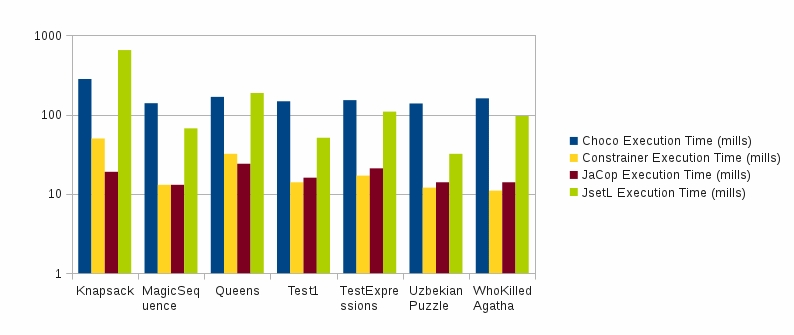
\includegraphics[scale=.45]{img/grafico11.jpg}
\caption{test semplici, tempo impiegato.}
\end{figure}

Come si evince in figura, in questi semplici test JSetL si comporta abbastanza
bene, meglio di Choco in ben cinque casi su sette e praticamente un pareggio
sul problema delle otto regine. Si potrebbe dire che con poche variabili
l'ordine di grandezza del tempo impiegato coincide con Choco. Il discorso è
differente se si confronta con Constrainer o JaCoP, decisamente più performanti.

\begin{figure}[!ht]
\centering
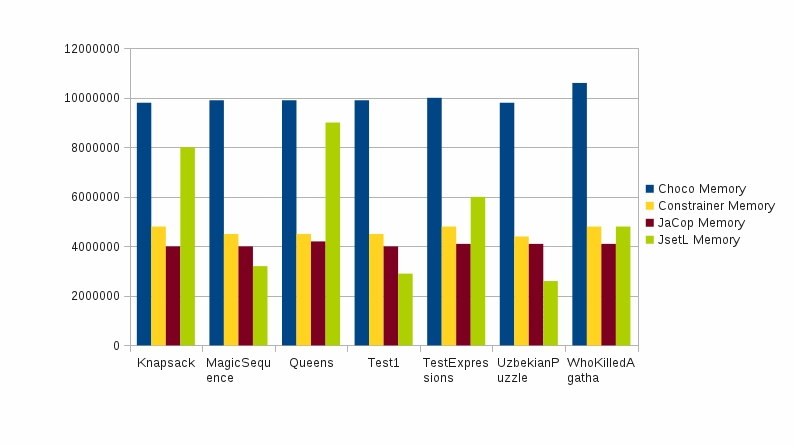
\includegraphics[scale=.45]{img/grafico12.jpg}
\caption{test semplici, memoria utilizzata.}
\end{figure}
Per quanto riguarda la memoria utilizzata invece, JSetL riesce ad essere
sempre sotto ai livelli di Choco e ben tre volte meglio di tutti gli altri.
I casi in cui viene utilizzata tanta memoria sono \emph{Knapsack} e
\emph{Queen}. Il primo probabilmente è causato dalla ricerca ottima
(\texttt{findOptimalSolution}), che non è direttamente supportata dal solver
JSetL, ma viene implementata mediante un algoritmo fatto ad \emph{hoc} che
espande e
propaga un vincolo all'interno del solver. Mentre la pesantezza
del problema delle regine, in termini di
memoria,  è indubbiamente dovuto alla presenza del
vincolo AllDifferent su tante variabili, e come questo è implementato in JSetL.

\subsection{Test complessi}
I test più complessi sono caratterizzati da un elevato numero di variabili
legate al problema o di supporto e da un elevato numero di vincoli, su tutti
quelli globali: Cardinality, AllDifferent, etc.

Sono stati catalogati come complessi poiché anche i solver che hanno dato prova
di essere i più performanti (JaCoP e Constrainer) risolvono i problemi dati
con tempi ben al di sopra dei precedenti.


Dal grafico si può notare che JSetL in questi casi è ben al di sopra degli altri
solver come tempo d'esecuzione. Nel test \emph{Golomb Rulers} il tempo
impiegato è circa il doppio rispetto a Choco e il triplo rispetto JaCoP e
Constrainer. In \emph{Magic Square} è ben dieci volte più lento degli altri,
mentre in \emph{Graph Coloring} circa sessanta. In questo caso però occorre dire
che JaCoP sembra non terminare, infatti la sua barra non è presente nel grafico.

\begin{figure}[!ht]
\centering
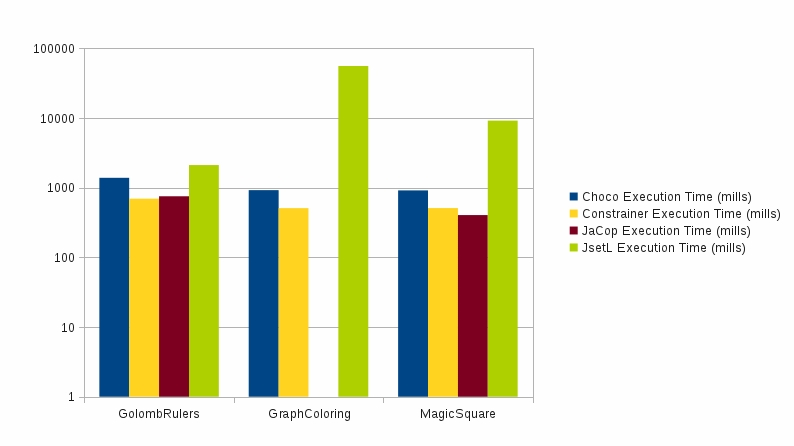
\includegraphics[scale=.45]{img/grafico13.jpg}
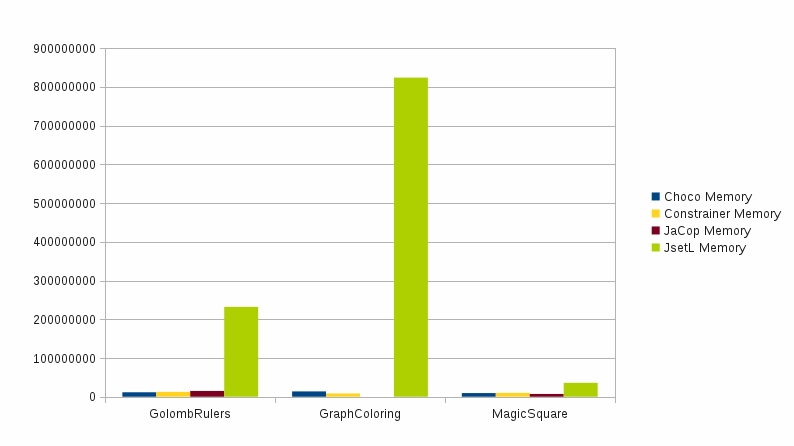
\includegraphics[scale=.4]{img/grafico14.jpg}
\caption{test complessi.}
\end{figure}

Per quanto riguarda la memoria utilizzata nei test complessi è invece evidente
che JSetL ne utilizzi veramente troppa rispetto agli altri solver e molto
probabilmente anche il deficit di prestazioni è dovuto a questo.



\backmatter
% Bibliografia.
\cleardoublepage
\phantomsection
\addcontentsline{toc}{chapter}{Bibliografia}
\begin{thebibliography}{}

\bibitem{specifiche} Jacob Feldman\\
        \emph{JSR-331 Java Constraint Programming API SPECIFICATION} \\
        \footnotesize \texttt{http://openrules.com/downloads/jsr331/JSR331.Specification.v081.pdf} \normalsize

\bibitem{tesiAmadini} Roberto Amadini \\
	\emph{Studio e realizzazione in Java di domini e regole per la risoluzione di vincoli su interi e insiemi di interi} \\
	\footnotesize \texttt{http://www.cs.unipr.it/Informatica/Tesi/Roberto\_Amadini\_20111109.pdf} \normalsize

\bibitem{prolog} Luca Console, Evelina Lamma, Paola Mello, Michela Milano \\
	\emph{Programmazione Logica e Prolog} \\
	UTET Libreria srl, 1997.

\bibitem{intArt} Stuart Russell, Peter Norvig \\
	\emph{Intelligenza Artificiale \\ Un approccio moderno - Volume 1} \\
	Pearson Education Italia S.r.l., 2005.


\bibitem{artClp} A. Dovier, C. Piazza, E. Pontelli, G. Rossi \\
	\emph{Sets and constraint logic programming} \\
	ACM TOPLAS 2000; 22(5):861-931.

\bibitem{artJsetl} Gianfranco Rossi, Elio Panegai, Elisabetta Poleo \\
	\emph{JSetL: a Java library for supporting declarative programming in Java} \\
	Software Practice \& Experience 2007; 37:115-149.

\bibitem{jsetlMan} Gianfranco Rossi, Roberto Amadini \\
         \emph{JSetL User's Manual Version 2.3}\\
         "Quaderni del Dipartimento di Matematica", n. 507, Università di Parma, 24 Gennaio 2012.

\bibitem{jacop} JaCoP - Java Constraint Programming solver \\
	\texttt{http://jacop.osolpro.com/}

\bibitem{sitoJava} Java Platform, Standard Edition 6: API Specification \\
	\texttt{http://java.sun.com/javase/6/docs/api/}

\bibitem{jsetl} JSetL Home Page \\
	\texttt{http://cmt.math.unipr.it/jsetl.html}

\bibitem{blog}  Constraint Programming Standardization Blog\\
	\texttt{http://cpstandard.wordpress.com/}


\end{thebibliography}


\end{document}
